\documentclass{article}
\usepackage[utf8]{inputenc}
\usepackage[brazil]{babel}
\usepackage{fancyheadings}
\usepackage{amsmath}
\usepackage{calrsfs}
\usepackage{enumerate}
\usepackage{amsmath, amsfonts, amssymb}
\usepackage{esint}
\usepackage{graphicx}
\usepackage{multicol}
\usepackage{tasks}
\usepackage[utf8]{inputenc}
\usepackage{mathrsfs} % Transformada de Laplace
\usepackage{gensymb}
\usepackage{anysize} 
\marginsize{ 1 centímetro }{2 }{ 4 em em}{6pt} 


    


\begin{document}

% capa
\begin{titlepage} %iniciando a "capa"
\begin{center} %centralizar o texto abaixo
    {\large Universidade Federal do Ceará}\\[0.2cm] %0,2cm é a distância entre o texto dessa linha e o texto da próxima
    {\bf \huge MATEMÁTICA POSCOMP}\\[5.1cm] % o comando \bf deixa o texto entre chaves em negrito. O comando \huge deixa o texto enorme
\end{center} %término do comando centralizar
{\large Aluno: Jonas Bezerra da Costa máximo}\\[0.7cm] % o comando \large deixa o texto grande
{\large Professor:Antônio Joel Ramiro de Castro}\\[4.2cm]
\begin{center}
    {\large Quixadá}\\[0.2cm]
    {\large 2019}
\end{center}
\end{titlepage}\newpage  %término da "capa"


{\bf \huge Sumário}\\\\

1 INTRODUÇÃO.................................................00

2 ESTRUTURA..................................................00

3 CÁLCULO....................................................00

4 LÓGICA.....................................................00

5 ÁLGEBRA....................................................00

6 PROBABILIDADE..............................................00

7 GRAFO......................................................00\newpage




{\bf \huge Estrutura}\newline




\noindent questão ) (ano da prova, questão da prva)\newline


$

    \noindent \textbf{Conteúdo para resolver}\newline
    \begin{cases}
        \mbox{aqui terá um breve resumo sobre o conteúdo nescesário para resolver as qiestões }     
    \end{cases}
$

$

    \noindent \textbf{Resolução da questão}\newline
    \begin{cases}
        \mbox{aqui terá a resolução da questão de uma forma bem detalhada}    
    \end{cases}
$
\vspace{50}

O capítulo de cálculo emgloba as áres de:\\
Pré-Cálculo, Cálculo 1, Cálculo 2, Cálculo 3, Equações Diferenciais Ordinárias (EDO), Geometria.\vspace{20}


O capítulo de lógica emgloba as áres de:\\
Matemática Básica, Matemática Discreta, Lógica.\vspace{20}


O capítulo de algebra emgloba as áres de:\\
Algebra.\vspace{20}


O capítulo de probabilidade emgloba as áres de:\\
Probabilidade, Estatística.

\newpage



































\newpage
\section{CÁLCULO}
\begin{enumerate}


\item (2018, 5) Calcule o limite de $$\lim_{h \to 0}(\sqrt{x^4 + x^2} + \sqrt{x^2 + 5x} - x² -x)$$ 

a) 1

b) 5

c) $\infty$

d) 0

e) 3\newline




\item (2018, 6) Determine os valores de a e b para que a função abaixo seja contínua em todo o
seu domínio:

\begin{center}
$

    f(x)=
    \begin{cases}
       $-3.\sin{x}$ \hspace{3} se \hspace{3} $x<-\frac{\pi}{2}$ \\
       
       $a.\sin{x}+b$ \hspace{3} se \hspace{3} $-\frac{\pi}{2} \leq x \leq \frac{\pi}{2}$\\
       
       $\cos{x}$ \hspace{3} se \hspace{3} $x> \frac{\pi}{2}$
      
    \end{cases}
$

\end{center}\newline


a) a=$\frac{3}{2}$; b=$\frac{3}{2}$

b) a=$-\frac{3}{2}$; b=$\frac{3}{2}$

c) a=$\frac{3}{2}$; b=$-\frac{3}{2}$

d) a=$-\frac{3}{2}$; b=$-\frac{3}{2}$

e) a=$\frac{2}{3}$; b=$\frac{3}{2}$



\item (2018, 8) O ponto $P(3, 45^{\circ}, 60^{\circ})$ está expresso em coordenadas esféricas. Encontre suas coordenadas cartesianas:\\

$Ax = r . \sin{(\theta)}.\cos{(\varphi)}$

$Ay= r.\sin{(\theta)}.\sin{(\varphi)}$

$Az = r.\cos{(\theta)}$\\

a)$P\bigg(\frac{3\sqrt{2}}{4}, \frac{3\sqrt{6}}{4}, \frac{3\sqrt{2}}{2} \bigg) $

b)$P\bigg(\frac{3\sqrt{6}}{4}, \frac{3\sqrt{2}}{4}, \frac{3\sqrt{2}}{4} \bigg) $

c)$P\bigg(\frac{3\sqrt{2}}{2}, \frac{3\sqrt{2}}{4}, \frac{3\sqrt{2}}{2} \bigg) $

d)$P\bigg(\frac{3\sqrt{2}}{4}, \frac{3\sqrt{2}}{2}, \frac{3\sqrt{2}}{2} \bigg) $

e)$P\bigg(\frac{3\sqrt{2}}{4}, \frac{3\sqrt{6}}{4}, \frac{3\sqrt{6}}{4} \bigg) $\newline





\item (2018, 10) A primitiva de $\int \frac{x}{\sqrt{x^2 +1}} dx $ é:\newline

a) $(X^2 + 1)^{-1} + C$

b) $\sqrt{X^2 + 1} + C$

c) $X^2 + 1 + C$

d) $X^2 + C$ 

e) C\newline



\item (2017, 4) Em relação às figuras geométricas planas, a circunferência possui excentricidade:

a) e = 0

b) e = 1

c) $e < 1$

d) $e > 1$

e) e = $\sqrt{2}$\newline






\item (2017, 5) Sobre o seguinte conjunto A =\{$x  \epsilon R \frac{|x-2|}{x^2}>1\}$, verifica-se que:\newline

a) Não tem máximo, e o mínimo é 0.

b) O máximo é 1 e não possui mínimo.

c) O máximo é 1 e o mínimo é 0.

d) É um conjunto vazio.

e) O máximo é 1 e o mínimo é -2.\newline





\item (2017, 6) limite de $\sqrt[n]{\frac{n^2+1}{n^7-2}}$ quando $n\rightarrow \infty$ é:

a) 1

b) 0

c) $\infty$

d) 2/7

e) 1/2\newline




\item (2017, 7)Qual é a solução do seguinte sistema de equações $
f(n) = \left \{ \begin{matrix} 
3x_1 + 2x_2 + 5x_3 =1\\
4x_1 + 3x_2 + 6x_3 =2\\
5x_1 + 4x_2 + 7x_3 =3\\
6x_1 + 7x_2 + 8x_3 =4\\
\end{matrix} \right.$? \newline

a) $(x_1 , x_2 , x_3 ) = (1,1,0)$

b) $(x_1 , x_2 , x_3 ) = (2,0, -1)$

c) $(x_1 , x_2 , x_3 ) = (0,1,0)$

d) $(x_1 , x_2 , x_3 ) = (2,1,0)$

e) $(x_1 , x_2 , x_3 ) = (2,2, -1)$\newline








\item (2017, 8) Dadas as retas r $\equiv 3x + y - 1 = 0$ e $s \equiv 2x + my - 8 = 0 $, qual dos seguintes é um
valor de m que faz com que as retas r e s formem um ângulo de $45^\circ$?

a) 1

b) $\sqrt{2}$

c) 0

d) -1

e) 2\newline







\item (2016, 1) Uma empresa de logística e transporte rodoviário tem três tipos de caminhões (tipo
1, tipo 2 e tipo 3), sendo que cada caminhão tem capacidade para transportar equipamentos com 3
diferentes dimensões, conforme o número de unidades correspondente, de acordo com o que está
descrito na tabela abaixo:\newline

% ######## init table ########
\begin{table}[h]
 \centering
% distancia entre a linha e o texto
 {\renewcommand\arraystretch{1.25}
 \begin{tabular}{ }

 \end{tabular} }
\end{table}


% ######## init table ########
\begin{table}[h]
 \centering
% distancia entre a linha e o texto
 {\renewcommand\arraystretch{1.25}
 \begin{tabular}{ l l l l }
  \cline{1-1}\cline{2-2}\cline{3-3}\cline{4-4}  
    \multicolumn{1}{|c|}{  \centering } &
    \multicolumn{1}{c|}{Dimensão A \centering } &
    \multicolumn{1}{c|}{Dimensão B \centering } &
    \multicolumn{1}{c|}{Dimensão C \centering }
  \\  
  \cline{1-1}\cline{2-2}\cline{3-3}\cline{4-4}  
    \multicolumn{1}{|c|}{Caminhão tipo 1 \centering } &
    \multicolumn{1}{c|}{1 \centering } &
    \multicolumn{1}{c|}{0  \centering } &
    \multicolumn{1}{c|}{1 \centering }
  \\  
  \cline{1-1}\cline{2-2}\cline{3-3}\cline{4-4}  
    \multicolumn{1}{|c|}{Caminhão tipo 2 \centering } &
    \multicolumn{1}{c|}{ 2 \centering } &
    \multicolumn{1}{c|}{2 \centering } &
    \multicolumn{1}{c|}{1 \centering }
  \\  
  \cline{1-1}\cline{2-2}\cline{3-3}\cline{4-4}  
    \multicolumn{1}{|c|}{Caminhão tipo 3 \centering } &
    \multicolumn{1}{c|}{1 \centering } &
    \multicolumn{1}{c|}{1 \centering } &
    \multicolumn{1}{c|}{2 \centering }
  \\  
  \hline

 \end{tabular} }
\end{table}\newline

A quantidade de caminhões carregados com a sua capacidade máxima que deve ser usada para
transportar, respectivamente, 23 equipamentos com a dimensão A, 18 equipamentos com a dimensão
B e 20 equipamentos com a dimensão C é:\newline

a) 4 caminhões do tipo 1; 7 caminhões do tipo 2 e 5 caminhões do tipo 3.

b) 5 caminhões do tipo 1; 6 caminhões do tipo 2 e 6 caminhões do tipo 3.

c) 3 caminhões do tipo 1; 7 caminhões do tipo 2 e 5 caminhões do tipo 3.

d) 1 caminhão do tipo 1; 5 caminhões do tipo 2 e 8 caminhões do tipo 3.

e) 5 caminhões do tipo 1; 7 caminhões do tipo 2 e 4 caminhões do tipo 3.\newline




\item (2016, 3)Os pontos A(2,3,4), B(1,5,6) e C(4,2,3) são os vértices de um triângulo de área:\newline

a) $\sqrt{3} cm^2$

b) $2\sqrt{3} cm^2$

c) $\frac{3\sqrt{2}}{2} cm^2$

d) $6\sqrt{3} cm^2$

e) $3\sqrt{3} cm^2$\newline



\item (2016, 4) O ângulo entre os vetores$\vec u $ = (2,2,0) e $\vec v$ = (0,3, -3) é:\newline

a) $ 0^\circ$

b) $ 30^\circ$

c) $ 45^\circ$

d) $ 60^\circ$

e) $ 90^\circ$ \newline



\item (2016, 5)Os valores críticos da função $y=f(x)=\frac{x^4}{4}-\frac{14}{3}x^3 + 20x^2 + 5$ são:

a) x=0, x=4 e x=10.

b) x=4 e x=10.

c) x=0, x=-4 e x=10.

d) x=0, x=-4 e x=-10.

e) x=0, x=4 e x=-10.\newline


\item (2016, 6) Um dos métodos iterativos para determinar as raízes de uma função é o Método de
Newton-Raphson, descrito por:\newline

$x_{n+1}=x_n -\frac{f(x_n)}{f'(x_n)} $\newline

Portanto, para determinar as raízes da função $ y = f(x) = x^3 -\sin{x}$ , temos a descrição da expressão algébrica na alternativa:\newline

a) $x_{n+1} = x_n -\frac{(x_ n^3 -\sin{(x_n)})}{(3x_n^2 -\cos{(x_n)})}$

b) $x_{n+1} = x_n -\frac{(x_ n^3 -\sin{(x_n)})}{(3x_n^2 +\cos{(x_n)})}$

c) $x_{n+1} = x_n -\frac{(x_ n^3 -\sin{(x_n)})}{(x_n^2 -\cos{(x_n)})}$

d) $x_{n+1} = x_n -\frac{(x_ n^3 -\sin{(x_n)})}{(3x_n^2 -\sin{(x_n)})}$

e) $x_{n+1} = x_n -\frac{(x_ n^3 -\sin{(x_n)})}{(6x_n^3 -\cos{(x_n)})}$





\item (2016, 7)A equação que representa a forma da cônica na imagem abaixo é:\newline

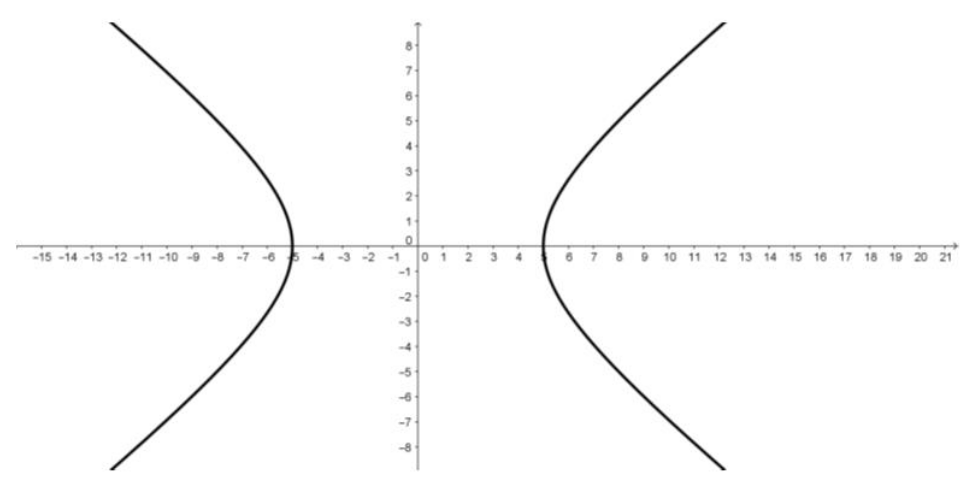
\includegraphics[width=10 cm]{07-2016.png}\newline

a)$x^2 = 4y + 4$

b)$ \frac{x^2}{25} + \frac{y^2}{16} = 1$

c)$ \frac{x^2}{25} - \frac{y^2}{16} = 1$

d)$ \frac{x^2}{16} + \frac{y^2}{25} = 1 $

e)$ \frac{x^2}{16} - \frac{y^2}{25} = 1 $\newline






\item (2016, 10)A área da região limitada pelo gráfico da função $f(x) = -2x^3$ e $g(x) = -8x,$ conforme
descrito na imagem abaixo, é:\newline

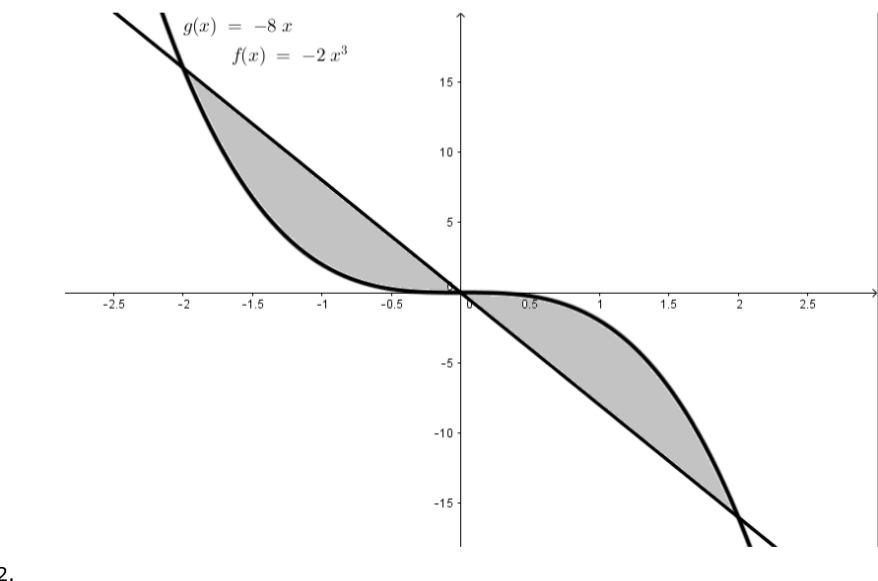
\includegraphics[width=10 cm]{10-2016.png}\newline

a) 32

b) 24.

c) 16.

d) 8.

e) 4.\newline



\item (2015, 3) Entre o centro da circunferência, cuja equação em coordenadas polares é dada por $r=2 \cos\theta +2 \sqrt{3}  \sin\theta,$ e a reta $-2 x+ y=4 $, a distância é:

a)$ 6 -\sqrt{3}$

b) $\frac{6 -\sqrt{5}}{\sqrt{3}}$

c)$ 6 -\sqrt{5}$

d)$ \frac{6 -\sqrt{3}}{\sqrt{5}}$

e)$ \frac{12 -\sqrt{3}}{2\sqrt{5}}$\newline



\item (2015, 5) A figura a seguir representa parte do gráfico da derivada de uma função polinomial.


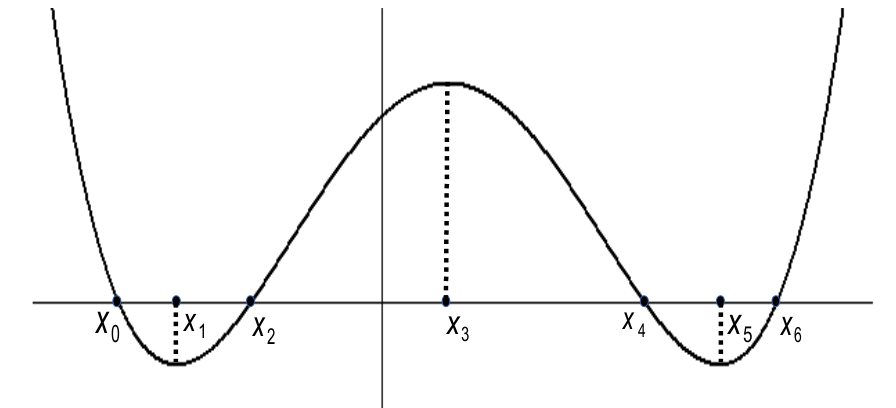
\includegraphics[width=10 cm]{05-2015.png}\newline

De acordo com os dados apresentados neste gráfico, a função polinomial apresenta\newline

a) um ponto de mínimo local em $x_1$ .

b) um ponto de máximo local em $x_4$ .

c) um ponto de inflexão em $x_0$ .

d) um ponto de mínimo local em $x_5$ .

e) um ponto de máximo local em $x_6$ .



\item (2015, 6) As mudanças de coordenadas, obtidas por meio de transformações, são muito utilizadas na resolução de equações diferenciais. Considere a chamada equação da onda\newline

$\frac{\partial^2 F}{\partial x^2} - \frac{1}{c^2}\frac{\partial^2 F}{\partial t^2} =0$\newline

onde F(x,t) é uma função contínua com derivadas parciais contínuas até segunda ordem e c é uma constante.
Aplicando-se uma mudança de coordenadas, mediante a transformação\newline

$u=x+ct$ e $v=x-ct$\newline

a equação da onda pode ser escrita como\newline

a) $F_{uu} + F_{vv} =0$

b) $F_{uu} - F_{vv} =0$

c) $F_{uv} =0$

d) $F_{uu} -2 F_{uv} + F_{vv} =0$

e) $F_{vv} -2 F_{uv} - F_{uu} =0$\newline




\item (2015, 8) Um prisma é delimitado pelos planos de equações x=0, z=0, y=0, y=5 e 3 x+7 z=21.
O valor numérico do volume desse prisma é:\newline


a) 37,5

b) 39,5

c) 43,5

d) 47,5

e) 52,5\newline




\item (2015, 9) Segundo o conceito de relações,\newline

a) a relação x+ y=10 define uma relação de equivalência sobre o conjunto dos números naturais.

b) a relação de congruência módulo m sobre Z dada por $x R y \Leftrightarrow x \equiv y$ $mod ( m)$ , onde $m\in Z$ e $m  > 1$, determina em Z um conjunto quociente que possui exatamente m-1 elementos.

c) a relação de divisibilidade sobre N dada por $x R y \Leftrightarrow x|y$ é uma relação de ordem total.

d) a relação sobre R definida por $xRy \Leftrightarrow x \leq y$ é uma relação de ordem total.

e) a relação de equivalência R={( a , a) ,(b , b ) ,(c , c) ,(a , c) ,(c , a)} possui exatamente três classes de equivalência.\newline



\item (2015, 10) O trabalho realizado pelo campo diferenciável 
$F ( x , y)= ( x^4 - y^3 , x^3 + y^5 )$para percorrer a circunferência $x^2 + y^2 =1$, no sentido anti-horário, é:\newline


a) $ 3\pi$

b) $ 3\frac{\pi}{2}$

c) $ 3\frac{\pi}{4}$

d) $ 3\frac{\pi}{8}$

e) $ 3\frac{\pi}{16}$\newline



\item(2014, 4)Em relação à circunferência de centro (2, 1) e raio 2 no plano, assinale a alternativa correta.\newline


a) A reta y = $\frac{1}{2} x$ passa pelo centro dessa circunferência.

b) A reta y = 2x passa pelo centro dessa circunferência.

c) A reta y = 0 tangencia a circunferência.

d) A reta y = 2 passa pelo centro da circunferência.

e) A reta x = 0 passa pelo centro da circunferência.\newline




\item(2014, 5)Sabendo que $f (x) \frac{1}{4} \ln{\frac{1+x}{1_x}} = \sum_{m=0}^{x^2n+1}$, onde $|x|\leq 1$ , e considerando apenas os dois primeiros termos não nulos da série, assinale a alternativa correta.

a)$\lim_{x \to \infty} \frac{f(x)}{x^3} \approx \infty$, $\frac{d}{dx}f(x)\approx x + x^2$ e $\int_{0}^{1} f(x)dx \approx \frac{1}{12}$

b)$\lim_{x \to \infty} \frac{f(x)}{x^3} \approx \infty$, $\frac{d}{dx}f(x)\approx 1 + x^2$ e $\int_{0}^{1} f(x)dx \approx \frac{7}{12}$

c)$\lim_{x \to \infty} \frac{f(x)}{x^3} \approx \frac{1}{3}$, $\frac{d}{dx}f(x)\approx 1 + x^2$ e $\int_{0}^{1} f(x)dx \approx \frac{1}{12}$

d)$\lim_{x \to \infty} \frac{f(x)}{x^3} \approx \frac{1}{3}$, $\frac{d}{dx}f(x)\approx 1 + x^2$ e $\int_{0}^{1} f(x)dx \approx \frac{7}{12}$

e)$\lim_{x \to \infty} \frac{f(x)}{x^3} \approx \frac{1}{3}$, $\frac{d}{dx}f(x)\approx x + x^2$ e $\int_{0}^{1} f(x)dx \approx \frac{7}{12}$\newline






\item(2014, 6) \newpage










\item(2014, 10)Em relação à função $f (x, y) = x^2 - 2xy + 2y$, definida no intervalo compacto $D = \{(x, y) \in R^2 | 0 \leq x \leq 3$ e $0 \leq y \leq 2\}$, considere as afirmativas a seguir.

I. (1, 1) $\in R^2$ é um ponto crítico de f , mas f (1, 1) não é nem um ponto de máximo nem um ponto de
mínimo absoluto de f .

II. (1, 1) $\in R^2$ é um ponto crítico de f e f (1, 1) é um ponto de mínimo absoluto de f .

III. f (0, 0) e f (0, 2) são, respectivamente, mínimo e máximo absoluto de f .

IV. f (3, 2) = f (1, 1) não são nem ponto de máximo nem ponto de mínimo absoluto de f .

Assinale a alternativa correta.

a) Somente as afirmativas I e II são corretas.


b) Somente as afirmativas I e IV são corretas.

c) Somente as afirmativas III e IV são corretas.

d) Somente as afirmativas I, II e III são corretas.

e) Somente as afirmativas II, III e IV são corretas.\newline







\item(2014, 16)
Com base nos conhecimentos sobre a definição de ponto fixo, relacione as funções reais, na coluna da
esquerda, com seus respectivos conjuntos de pontos fixos, na coluna da direita.

a) (I) $f (n) = n$  \hspace{70} a) \{0, 1\}

b) (II) $f (n) = n + 1$     \hspace{50} b) \{0, 3\}

c) (III) $f (n) = n^2 $    \hspace{60}     c) \{1\}

d) (IV) $f (n) = n^2 - 2n $  \hspace{37} d) $\phi$

e) (V) $f (n) = n^ + n -1$ \hspace{40}  e) R
 
 
Assinale a alternativa que contém a associação correta.

a) I-A, II-C, III-B, IV-E, V-D.

b) I-B, II-C, III-D, IV-E, V-A.

c) I-B, II-D, III-A, IV-C, V-E.

d) I-E, II-B, III-D, IV-C, V-A.

e) I-E, II-D, III-A, IV-B, V-C.\newline



\item(2013, 1) Um determinado serviço pode ser realizado por dois programas distintos, $P_1$ e $P_2$ , utilizando algoritmos diferentes. O usuário fornece aos programas um número natural $n  \geq 1$ e os programas fornecem uma resposta. O tempo que o programa $P_1$ demora para responder é dado pela fórmula $T_1 (n) = n^4$. Já o tempo da resposta do programa P 2 é calculado por $T_2 (n) = 2^{n-1}$. Em relação aos programas $P_1$ e $P_2$ , assinale a alternativa correta.

a)Como $\lim{n \to \infty}$ $t_2 (n) = \infty$, então $\lim{n \to \infty} \frac{t_2(n)}{t_1(n)} = \frac{\lim{n \to \infty} t_2(n)}{\lim{n \to \infty}t_1(n)}$ = 1 e, por isso, o programa $P_2$ é mais rápido que o programa $P_1$ , para entradas maiores do que um certo número natural N .

b) Como $\lim{n \to \infty}$ $t_2 (n) = \infty$, então $\lim{n \to \infty} (t_2(n) - t_1(n)) =\lim{n \to \infty} (t_2(n)) - \lim{n \to \infty}(t_1(n))$ = 0 e, por isso,ambos os programas levam o mesmo tempo para dar uma resposta.

c) Como $\lim{n \to \infty}$ $(t_2(n)) = \lim{n \to \infty}(t_1(n)) = \infty$ , então, a partir de um certo número natural N , ambos os programas levam o mesmo tempo para dar uma resposta.

d)Como $\lim{n \to \infty}$ $[t_2(n) - t_1(n)] = \infty$, então o programa P 1 é mais rápido que o programa P 2 para entradas maiores do que um certo número natural N .

e) Como $\lim{n \to \infty}$ $[t_2(n) - t_1(n)] = \infty$ , então o programa $P+-2$ é mais rápido que o programa $P_1$ para entradas maiores do que um certo número natural N .v\newline






\item(2013, 4) Em relação à função $f (x, y) =\sqrt{4-x^2 - y^2}$ , considere as afirmativas a seguir.

I. O domínio de f é dado por $D = \{(x, y) ∈ R x R | x^2 + y^2 \leq 4\}.$

II. $\frac{\partial}{\partial x} f (x, y) = - \frac{2x}{\sqrt{4-x^2-y^2}}$

III. $\frac{\partial}{\partial x} f (x, y) = \frac{\partial}{\partial y} f (x, y) para todo (x, y)$ pertencente ao domínio da função f .

IV. $\sqrt{4-x^2-y^2}$ = 3 é uma curva de nível da função f .

Assinale a alternativa correta.

a) Somente as afirmativas I e II são corretas.

b) Somente as afirmativas I e IV são corretas.

c) Somente as afirmativas III e IV são corretas.

d) Somente as afirmativas I, II e III são corretas.

e) Somente as afirmativas II, III e IV são corretas.\newline









\item(2013, 10)Considere o gráfico da função $f : [a, e] \rightarrow R $a seguir.

\includegraphics[width=10 cm]{2015.png}\newline


Com relação a esse gráfico, atribua V (verdadeiro) ou F (falso) às afirmativas a seguir.

( ) 0 é ponto de inflexão no domínio de f

( ) 0 é ponto crítico no domínio de f

( ) c é ponto de máximo local no domínio de f

( ) f não é diferenciável em d

( ) e não é ponto extremo no domínio de f

Assinale a alternativa que contém, de cima para baixo, a sequência correta.

a) V, V, F, V, F.

b) V, F, V, V, F.

c) V, F, F, F, V.

d) F, V, V, V, F.

e) F, V, V, F, V.\newline



\item(2012, 3) Leia a definição a seguir. A série de potências $a+0 + a_1 + \frac{x}{1!}+ \frac{x^2}{2!}+ \frac{x^3}{3!}+ \frac{x^4}{4!}+... + ar\frac{x^r}{r!}+ ...$ é a função geradora exponencial da sequência $(a_0 , a_1 , ..., a_r , ...)$

Com base nessa definição, considere as afirmativas a seguir.

I. $e^{2x} $ é a função geradora exponencial para a sequência $a_k = 2^k$ .

II. $e^x - e^{-x}$ é a função geradora exponencial para a sequência (0, 2, 0, 2, 0, 2, ...).

III. $e^x - x^2$ é a função geradora exponencial para a sequência (1, 1, 0, 1, 1, 1, ...).

IV. $1+ \frac{x}{1!} + \frac{x^2}{2!}$ é a função geradora exponencial para a sequência (1, 1, 1, 1, 0, 0, 0, 0, ...).

Assinale a alternativa correta.


a)Somente as afirmativas I e II são corretas.

b)Somente as afirmativas I e IV são corretas.

c)Somente as afirmativas III e IV são corretas.

d)Somente as afirmativas I, II e III são corretas.

e)Somente as afirmativas II, III e IV são corretas.\newline



\item(2012, 4)Seja o conjunto A = $\{a \in Z|100 \leq a \leq 90.000\}$. Assinale a alternativa que apresenta, corretamente, os elementos do conjunto A que não são divisíveis nem por 3, nem por 5, nem por 9.

a)41.953

b)42.000

c)47.947

d)48.000

e)48.053\newline



\item(2012, 6)Sejam $(x_n)$ e $(y_n)$ duas sequências reais. Com relação a essas sequências, considere as afirmativas a seguir.

I. Se $\lim x_n$ = l então $\lim -x_n $= -l.

II. Se a, b são números reais e $\lim_{n \rightarrow \infty}x_n $= a e $\lim_{n \rightarrow \infty} y_n = b$ então $\lim_{n \rightarrow \infty} (x_n + y_n ) = a + b.$

III. Se $(x_n)$ é uma sequência limitada então $(x_n)$ é convergente.

IV. Se $(y_n)$ = $\frac{1}{n}$ então $\lim_{n \rightarrow \infty} y_n = 1.$

Assinale a alternativa correta.

a) Somente as afirmativas I e II são corretas.

b) Somente as afirmativas I e IV são corretas.

c) Somente as afirmativas III e IV são corretas.

d) Somente as afirmativas I, II e III são corretas.

e) Somente as afirmativas II, III e IV são corretas.\newline




\item(2012, 7)Assinale a alternativa que apresenta, corretamente, as equações das retas tangentes à circunferência de centro C = (1, 0) e raio 2, e que são paralelas à reta x + y - 1 = 0.

a) x - y = 1 e -x + y = -1

b) x + y = 1 + $\sqrt{2}$ e x + y = 1 - $\sqrt{2}$

c) y-x = 1+ $\sqrt{2}$ e y - x = 1 -$\sqrt{2}$

d) 2x + 2y = 2 e 2x + 2y = -2

e) 2x + 2y =2$\sqrt{2}$ e 2x + 2y = -2 $\sqrt{2}$







\item(2012, 9) Seja$
f(n) = \left\{ \begin{matrix} 
 \frac{x^2}{x^2 + 1} se x \geq 0 \\
 \frac{x}{x^2 -1} se z <0
\end{matrix} \right.$
Com relação a essa função, assinale a alternativa correta.

a) A função f é contínua para todo $x \in R$.

b) A função f é diferenciável para todo $x \in R$.

c) Não existe $\lim_{x \rightarrow 0} f (x)$.

d) x = 1 é uma assíntota vertical de f .

e) A função f tem duas assíntotas horizontais.\newline





\item(2012, 10)Sejam as curvas $y = x - 1$ e $x^2 + y^2 - 2x - 2y - 3 = 0.$ Assinale a alternativa que apresenta, corretamente, as coordenadas do ponto médio do segmento de reta determinado pelos pontos de interseção dessas curvas.

a) $( \frac{1}{2}, -\frac{1}{2})$

b) (1,2)

c) $( \frac{3}{2}, \frac{1}{2})$

d) $( \frac{3}{2}, 1)$

e) (0,-1)\newline



\item(2012, 11)Assinale a alternativa que apresenta, corretamente, o valor da área da região limitada por $y = \sin(x)$, $y = \cos(x)$, $x = 0$ e $x = \pi$.

a) $2\sqrt{2} - 2$

b) $\sqrt{2}$

c) 2

d) $2 \sqrt{2}$

e) $2\sqrt{2} + 2$\newline




\item(2012, 13)Uma empresa deseja fabricar uma lata cilíndrica fechada com volume igual a 2000π cm 3 , utilizando a menor quantidade possível de material.

Assinale a alternativa que apresenta, correta e respectivamente, as dimensões, altura h e raio r, em cm,
que essa lata deve ter.

a) h = 10 ; r = 20

b) h = 20 ; r = 10

c) h = 40 ; r = 5 $\sqrt{2}$

d) h = 50 ; r = 2 $\sqrt{10}$

e) h = 80 ; r = 5\newline




\item(2011, 2) Sejam a e b números reais não nulos. As duas retas perpendiculares à reta $\frac{x}{a} + \frac{y}{b} = 1$ que formam triângulos de área $|ab|$ com os eixos ordenados são descritas pelas equações:

a) $ax - by = 1 e -ax + by = 1$

b) $\frac{x}{a} - \frac{y}{b} = 1$ e $\frac{y}{b} - \frac{x}{a} =1$

c) $\frac{x^2}{a^2} + \frac{y^2}{b^2} = 1$ e $\frac{y^2}{b^2} - \frac{x^2}{a^2} =1$

d) $\frac{x}{a} - \frac{y}{b} = \sqrt{2}$ e $\frac{y}{b} - \frac{x}{a} =\sqrt{2}$

e) $\frac{x}{|a|} + \frac{y}{|b|} = \sqrt{2}$ e $\frac{y}{|b|} + \frac{x}{|a|} =-\sqrt{2}$\newline








\item(2011, 4) O valor de x > 0, pertencente ao primeiro quadrante, para a expressão $2 + 2\cos(x) + 2\cos(x)\cos(x) + 2\cos(x)\cos(x)\cos(x) + 2\cos(x)\cos(x)\cos(x)\cos(x) + ... = 4$ é:

a) 0

b) $\frac{\pi}{6}$

c) $\frac{\pi}{3}$

d) $\frac{\pi}{2}$

e) $\pi$\newline






\item(2011, 5) Em muitos problemas práticos, deseja-se encontrar a reta r(x) = ax + b que melhor se ajusta a um conjunto $\{(x 1 , y 1 ), (x 2 , y 2 ), ..., (x n , y n )\}$ de pontos no plano. No método dos mínimos quadrados, os coeficientes a e b da reta são determinados de modo que o erro, dado pela soma do quadrado da diferença entre y i e $r(x_i )$, isto é,

Erro (a,b) =$\sum_{i=1}^n (y_i -r(x_i))^2$

seja o menor possível.

A tabela a seguir mostra o conjunto de pontos $\{(-3, -3), (-2, -2), ..., (2, 6), (3, 6)\}$ no plano.


\includegraphics[width=10 cm]{2015.png}\newline


A reta que melhor se ajusta aos dados apresentados nessa tabela, no sentido dos mínimos quadrados, é:

a) $r(x) = x$

b) $r(x) =\frac{15}{7}x$

c) $r(x) = \frac{3}{2}x + \frac{3}{2}$

d) $r(x) =\frac{45}{28}x + \frac{15}{7}$

e) $r(x) =\frac{7}{2}x + \frac{45}{7}$\newline








\item(2011, 6) O problema de determinar um vetor normal a um triângulo ou polígono é muito comum em computação gráfica. Dado o triângulo formado pelos pontos A(1, 2, 3), B(3, 2, 1) e C(1, 1, 1), um vetor normal, n, a esse triângulo é dado por:

a) $n = [-2, 4, -2]^T$

b) $n = [0, 0, 4]^T$

c) $n = [2, -1, -4]^T$

d) $n = [3, 4, 5]^T$

e) $n = [5, 5, 5]^T$ \newline








\item(2011, 7)Com base em $f (x, y, z) = x^2 e^y + 2zy$, uma função real de três variáveis reais, considere as afirmativas a seguir.


I. O ponto P 0 = (1, 0, 1) é um ponto crítico de f .

II. A função f é contínua no ponto P 0 = (1, 0, 1).

III. A direção unitária em que f cresce mais rapidamente no ponto $P_0 = (1, 0, 1) é \frac{2}{\sqrt{13}} \vec i + \frac{3}{\sqrt{13}}\vec j$

IV. O vetor gradiente de f no ponto P 0 é nulo se, e somente se, P 0 = (0, 0, 0).

Assinale a alternativa correta.

a) Somente as afirmativas I e II são corretas.

b) Somente as afirmativas I e III são corretas.

c) Somente as afirmativas III e IV são corretas.

d) Somente as afirmativas I, II e IV são corretas.

e) Somente as afirmativas II, III e IV são corretas.\newline







\item(2011, 8)Relacione a equação em coordenadas polares da coluna da esquerda com a figura geométrica correspondente apresentada na coluna da direita.


\includegraphics[width=10 cm]{2015.png}\newline


Assinale a alternativa que contém a associação correta.

a) I-A, II-C, III-D, IV-E, V-B.

b) I-A, II-D, III-B, IV-C, V-E.

c) I-B, II-C, III-E, IV-A, V-D.

d) I-B, II-E, III-A, IV-D, V-C.

e) I-D, II-E, III-C, IV-B, V-A.\newline



\item(2011, 9) Considere o polinômio $p_n (x) = a_n x^n + ... + a_1x + a_0$ em seu formato padrão que pode ser escrito no formato encadeado $p_n (x) = x(x(...x(x(a_nx + a_{n−1}] ) + a_{n−2} ) + ... + a_2 ) + a_1 ) + a 0$ , colocando a variável x em evidência num número finito de vezes até que não seja mais possível fazê-lo.

Considerando que todos os coeficientes do polinômio são diferentes de zero, é correto afirmar que o total
de operações de adição e multiplicação para obter o valor de $p_{100} (5)$ é:

a) Duas vezes maior no formato encadeado que no padrão.

b) Igual no formato padrão e no encadeado.

c) Impossível de ser calculado.

d) Maior no formato encadeado que no padrão.

e) Maior no formato padrão que no encadeado.\newline





\item(2011, 10) A proporção de computadores acessando um provedor em um dado instante t a partir das 8 horas é dada por

$N(t)=\frac{1}{1+3e^{-kt}}$

onde o instante t é dado em horas e k é uma constante positiva. A proporção estimada de computadores acessando este provedor ao meio-dia é de:

a) $\frac{1}{k} \ln (2 + e^{4k})$

b) $\frac{1}{k} \ln \frac{(3e^{12k} + 1)}{4} $

c) $\frac{1}{k} \ln \frac{(3e^{12k} + 1)}{(3 + e^{8k})} $

d) $\frac{1}{k} \ln \frac{(3 + e^{12k})}{4} $

e) $\frac{1}{k} \ln \frac{(3 + e^{12k})^{3k}}{4} $\newline


\item(2011, 11) Sobre a função $f : R \rightarrow (-1, 1)$ definida pela lei $f (x)=\frac{x}{1+|x|}$ é correto afirmar:

a) f é bijetora.

b) f é decrescente.

c) f não é injetora, mas é sobrejetora.

d) f não é sobrejetora, mas é injetora.

e) f não é sobrejetora nem injetora.\newline




\item(2011, 12) Com base na função $f (x) = 6x^{3/2} - x^2 - 1$, considere as afirmativas a seguir.

I. f tem um zero no intervalo [0,1]

II.$\lim_{x \rightarrow +\infty} f (x) = +\infty$

III. f assume o valor máximo no ponto $x =\frac{81}{4}$

IV. f possui uma descontinuidade em zero

Assinale a alternativa correta.

a) Somente as afirmativas I e II são corretas.

b) Somente as afirmativas I e III são corretas.

c) Somente as afirmativas III e IV são corretas.

d) Somente as afirmativas I, II e IV são corretas.

e) Somente as afirmativas II, III e IV são corretas.\newline





\item(2010, 2)Considere o triângulo de vértices $A = (0 , 6)$ , $B = (4 , 10)$ e $C = (2 , 2)$ .
O ponto de interseção das medianas tiradas do vértice B e do vértice C é:

a) (2 , 6)

b) (3 , 8)

c) (4 , 6)

d) (5 , 4)

e) (6 , 2)



\item(2010, 5)Considere ∫ os conjuntos de polinômios $A = {1 , x, 3x^2 - 1 , 5x^3 - 3}$ e $B = {1 , x, x^2 , x^3 }$ e o produto interno 

$< p,q>= \int_{-1}^{1} p(x)q(x)dx$.

Com base no enunciado, considere as afirmativas a seguir.

I. A é um conjunto linearmente independente.

II. B é um conjunto linearmente independente.

III. A é a base ortogonal do conjunto de polinômios de grau até 3.

IV. B é a base ortogonal do conjunto de polinômios de grau até 3.

Assinale a alternativa correta.

a) Somente as afirmativas I e II são corretas .

b) Somente as afirmativas I e IV são corretas.

c) Somente as afirmativas III e IV são corretas.

d) Somente as afirmativas I, II e III são corretas.

e) Somente as afirmativas II, III e IV são corretas.



\item(2010, 6) Considere que $x_0 , x_1 , ...., x$ são pontos igualmente espaçados de h , onde $n \in N$ (conjunto dos números naturais), $n \geq 1$ e n  é um número par; $h > 0$ é a distância entre dois pontos quaisquer consecutivos

$x_j , x_{j +1} , j = 0 , ..., n - 1; h = x_{j +1} - x_j$ 

Sendo f uma função contínua de uma variável real, com valores tabelados da seguinte forma: $y_i = f ( x_i ) = 100$ para $i = 0 , 2 , 4 ..., n - 2 , n$ (índices pares) e $y_1 = f ( x_i ) = 200$ para $i = 1 , 3 , 5 ..., n - 1$ (índices ímpares), ∫ então, aplicando a regra dos trapézios generalizada para determinar o valor aproximado da integral $\int_{x_0}^{x_n} f(x) dx$ ,este valor resultará em:\newline

a) 50 nh

b) 100 nh

c) 150 nh

d) 200 nh

e) 300 nh


\item(2010, 7) A posição de uma partícula no instante $t \leq 0, t\in [0, 2\pi]$ que se desloca em função do tempo t em segundos,ao longo de uma reta coordenada, é dada por:

$s(t) = \cos{(2t + \frac{\pi}{4})}$
 
Determine os instantes em que a velocidade (em m/s ) é extrema (máxima/mínima) para a partícula, utilizandose de informações das derivadas primeira e segunda da velocidade.

a) $t=\frac{\pi}{8}s$ é o instante de velocidade mínima  e $t=\frac{5\pi }{8}s$ é o instante de valocidade máxima 

b) $t=\frac{\pi}{8}s$ é o instante de velocidade máxima  e $t=\frac{5\pi }{8}s$ é o instante de valocidade mínima 

c) $t=\frac{\pi}{4}s$ é o instante de velocidade máxima  e $t=\frac{5\pi }{4}s$ é o instante de valocidade mínima

d) $t=\frac{\pi}{4}s$ é o instante de velocidade mínima  e $t=\frac{5\pi }{4}s$ é o instante de valocidade máxima 

e) $t=\frac{3\pi}{8}s$ é o instante de velocidade mínima  e $t=\frac{7\pi }{8}s$ é o instante de valocidade máxima \newline





\item(2010, 19)Realizou-se uma brincadeira com n crianças, que receberam uma bexiga (balão) vazia cada uma, para então encherem até onde achassem que não estouraria. A brincadeira consistia, então, em determinar uma estratégia que estabelecesse a ordem na qual os balões atingiriam o teto do salão.

Considerando a quantidade de ar em cada bexiga e assumindo que seja possível determinar qual bexiga estava mais cheia de ar, quando comparadas duas a duas, quantas comparações, no máximo, seriam necessárias para soltar todos os balões, escolhendo de cada vez o balão precisamente mais cheio de ar?

a) $\log n$

b) $n^2 \log n$

c) $2^n$

d) $n^2$

e) $5n + 2$ \newline





\item(2009, 5)Considere as seguintes afirmativas:

I. As bissetrizes de dois ângulos adjacentes suplementares, i.e., que somam
$180^\circ$, são perpendiculares.

II. Se $\vec u$ e $\vec v$ são vetores paralelos não nulos, então existe $\lambda$ real tal que $\vec u = \lambda \vec v$

III. As medianas de um triângulo passam por um mesmo ponto.

IV. A área do triângulo com lados de comprimento a, b, c é dada por $\frac{1}{2}abc \cos{(\alpha)}$, onde $\alpha$ é o ângulo entre os lados de tamanho a e b.\newline

Assinale a quantidade de afirmativas CORRETAS.\newline

a) 0

b) 1

c) 2

d) 3

e) 4\newline





\item(2009, 7)Em um cabo de fibra ótica a quantidade de informação I que passa por ele durante a
hora h , é aproximada pela função\newline

$I(h) = 50 - 10 \sin{\frac{\pi h}{12}}$\newline

Calcule o horário de pico de tráfego de informação no período de 9h às 21h.\newline

a) 18 horas.

b) 6 horas.

c) 9 horas.

d) 6 horas e 18 horas.

e) Nenhuma das respostas anteriores.\newline





\item(2009, 8)A quantidade de acessos por mês a um portal de internet ao longo do tempo t em
meses, é estimada pela função\newline

$f(t)= \frac{4t^2 + 3t}{t^2 + 4t + 6}x100$\newline

Em quantos meses o número de acessos atinge ou ultrapassa 200 e para qual valor
tende a quantidade de acessos quando t tende ao infinito?\newline


a) 1,5 mês e 400 acessos.

b) 1,5 mês e 4000 acessos.

c) 4 meses e 4000 acessos.

d) 4 meses e 400 acessos.

e) 4 meses e 40000 acessos.\newline



\item(2009, 18) Calcule o valor de

$\int_0^4 (3x^2 + \frac{1}{\sqrt[2]{x}})dx $


a) 25,3333..

b) $34\sqrt[2]{2}$

c) 68

d) 69,3333...

e) Nenhuma das respostas anteriores.\newline









\item(2009, 19) Dado um conjunto S= \{ a,b,c,d\} , quantas são as possíveis relações de equivalência em S?

a) 4

b) 7

c) 8

d) 15

e) 16 \newline







\item(2009, 20) Três empresas, X,Y,Z estão competindo por clientes, usando uma campanha de
marketing.

Como reresultado dessa campanha, houve a seguinte mudança de clientes:\newline

7\% dos clientes de X trocam para Y

5\% dos clientes de X trocam para Z

14\% dos clientes de Y trocam para X

8\% dos clientes de Y trocam para Z

3\% dos clientes de Z trocam para X

5\% dos clientes de Z trocam para Y \newline


Se no início da campanha a distribuição de clientes era\newline


39\% para X

26\% para Y

35\% para Z \newline


Que operação matricial pode ser usada para representar o cálculo da distribuição de
clientes após o fim da campanha?\newline


a)$
 \left [ \begin{matrix} 
    \begin{array}{c}
    0,39 \\
    0,26  \\
    0,35  \\
\end{array}
\end{matrix} \right ]$ X
$
 \left [ \begin{matrix} 
    \begin{array}{ccc}
    0,12 & 0,14 & 0,03  \\
    0,07 & 0,22 & 0,05  \\
    0,05 & 0,08 & 0,08  \\
\end{array}
\end{matrix} \right ]$ \newline


b) $
 \left [ \begin{matrix} 
    \begin{array}{ccc}
    0,12 & 0,14 & 0,03  \\
    0,07 & 0,22 & 0,05  \\
    0,05 & 0,08 & 0,08  \\
\end{array}
\end{matrix} \right ]$ X
$
 \left [ \begin{matrix} 
    \begin{array}{c}
    0,39 \\
    0,26  \\
    0,35  \\
\end{array}
\end{matrix} \right ]$


c)$
 \left [ \begin{matrix} 
    \begin{array}{c}
    0,39 \\
    0,26  \\
    0,35  \\
\end{array}
\end{matrix} \right ]$ X
$
 \left [ \begin{matrix} 
    \begin{array}{ccc}
    0,88 & 0,14 & 0,03  \\
    0,07 & 0,78 & 0,05  \\
    0,05 & 0,08 & 0,92  \\
\end{array}
\end{matrix} \right ]$ \newline


d) $
 \left [ \begin{matrix} 
    \begin{array}{ccc}
    0,88 & 0,14 & 0,03  \\
    0,07 & 0,78 & 0,05  \\
    0,05 & 0,08 & 0,92  \\
\end{array}
\end{matrix} \right ]$ X
$
 \left [ \begin{matrix} 
    \begin{array}{c}
    0,39 \\
    0,26  \\
    0,35  \\
\end{array}
\end{matrix} \right ]$

e) Nenhuma das respostas anteriores.





\item(2008, 56) Considere a função f: $R \rightarrow R$ definida pela expressão $x^4 -4 x^3$ e assinale a afirmativa FALSA.


a) A função f é negativa, decrescente e com concavidade voltada para cima no
intervalo [-1,0] .

b) A função derivada f' é negativa, crescente e com concavidade voltada para baixo em
[-1,0] .

c) Em x = 0 , a função f tem um zero e um ponto de inflexão e a função derivada f' tem
um ponto de máximo local.

d) A reta tangente à curva y = f (x) em x = 3 é paralela ao eixo $ \overrightarrow{OX}$ .

e) O valor absoluto da área limitada pela curva y = f (x) que está abaixo do eixo $ \overrightarrow{OX}$  é 51,2 \newline




\item(2008, 57) Marcam-se 5 pontos sobre uma reta R e 8 pontos sobre uma reta S, paralela a R.
Quantos triângulos não degenerados existem com vértices em 3 desses 13 pontos?

a) 140

b) 80

c) 220

d) 440

e) 286\newline




\item(2008, 60)A proporção de computadores acessando um provedor em um dado instante t é dada pela equação $p(t)=\frac{1}{1+aexp^{kt}}$ em que P(t) é a proporção de computadores que estão 1 a exp kt acessando o provedor no instante t, a e k são constantes positivas com $a > 1$.

Calcule:

I. $\lim{t \to \infty} P (t)$

II. A taxa de aumento de computadores usando o provedor no instante t = 0. 

III. O tempo necessário para que 80\% dos computadores estejam acessando o provedor.

Assinale a alternativa que apresenta o cálculo CORRETO solicitado em I, II e III,
respectivamente.\newline

a) 0; $\frac{ka}{(1+a)^2}$; $\frac{-1}{k}\ln(1/4a)$

b)1; ka; $\frac{-1}{ka}$

c)1/a; $\frac{ka}{(1+a^2)}$; $\frac{-1}{ka}$

d) 1; $\frac{ka}{(1+a)^2}$; $\frac{-1}{k}\ln(1/4a)$

e) 1; $ka$; $\frac{-1}{k}\ln(1/4a)$\newline



\item(2008, 62)Um dispositivo eletrônico envia mensagens binárias no alfabeto (0,1) para um outro dispositivo de forma que o fim de uma transmissão é indicado por uma sequência de dois bits iguais a 1 .

Qual é o número máximo de mensagens binárias distintas que podem ter sido emitidas por esse dispositivo, sabendo que a transmissão parou ao ser enviado o décimo primeiro bit ?

a) $2^{11}$

b) $2^{10}$

c) 235

d) 144

e) 89 \newline










\item(2007, 1) A quantidade de soluções inteiras da equação $x + y + z = 20$ , com $x \geq 2, y \geq 2$ e $z \geq 2$, é

a) 120

b) 20

c) 231

d) 132

e) Essa equação não tem solução inteira.\newline






\item(2007, 6) Um trabalho de monitoramento do fluxo de acesso ao provedor de rede de deter- minada instituição foi efetivado durante uma hora, no perı́odo das 19 às 20 horas. A taxa estimada R(t) segundo a qual ocorre o acesso à rede é modelada pela expressão

$R(t) = 100(1 - 0, 0001t^2 )$ usuários/minuto,

em que t indica o tempo (em minutos) a partir das 19 h.
Considere as questões.

• Quando ocorre o pico no fluxo de acesso à rede ?

• Qual é a estimativa para o número de usuários que estão acessando a rede durante a hora monitorada ?

Assinale a alternativa que apresenta as melhores aproximações contendo as respostas CORRETAS a essas questões.

a) Das 20 : 30 às 21 : 30 horas; mais de 5.000 usuários.

b) Das 20 : 30 às 21 : 30 horas; menos de 5.000 usuários.

c) Das 19 : 30 às 20 : 30 horas; mais de 5.000 usuários.

d) Das 19 : 30 às 20 : 30 horas; menos de 5.000 usuários.

e) Nenhuma das aproximações contém as respostas.\newline



\item(2007, 7) considere a função $f :R \rightarrow R$ definida pela expressão:


$f(x)=
\left \{ \begin{matrix} 
    x^2, \hspace{30} \mbox{Se } x \leq 0\\
    x^2 +1, \hspace{25} \mbox{Se } x > 0
\end{matrix} \right.$ \newline

Com base nesses dados, assinale a alternativa que apresenta a afirmativa VERDADEIRA:

a) $\lim_{x \rightarrow 0^-} f'(x) = \lim_{x \rightarrow 0^+} f'(x)$ mas $ f'(0)$ não existe 

b) $\lim_{x \rightarrow 0^-} f(x) =0 $ e $\lim_{x \rightarrow 0^+} f(x) = 1 = f(0) $

c) $f(x)$ é contı́nua mas não é diferenciável.

d) $f'(x)$ é decrescente e $f(x) \geq 0$ se $X \in (-\infty,0) $

e) $\lim_{x \rightarrow \infty} f(x) = \infty$ e $\lim_{x \rightarrow -\infty} f'(x) = +\infty$\newline



\item(2007, 8)Assinale a alternativa que apresenta o comprimento do segmento de reta determinado pelos pontos de interseção de uma semi-reta, cuja origem está no ponto $P_1 (1, 2, 1)$ e cuja orientação é definida pelo vetor $d = (2, 1, 1)$, com a esfera centrada no ponto $C(31, 2, 21)$ e raio de $10\sqrt{3}$

a) $\frac{10}{3}$

b) $\frac{20}{3}\sqrt{6}$

c) $\frac{20}{3}$

d) $\frac{10}{3}\sqrt{3}$

e) $\frac{20}{3}\sqrt{3}$\newline




\item(2006, 4) A equaçao da reta tangente à parábola $y=x^{2}$ no ponto $(-2,4)$ é: 

a) $4x-y+4=0$

b) $4x+y+4=0$

c) $y-4x+4=0$

d) $4y-x+4=0$

e) $4y+x-4=0$ \newline



\item(2006, 5) Se $f(x)=\log _{a} 1 / x,$ então $f\left(a^{n}\right)$ é:

a) 1$/ n$

b) $-1 / n$

c) $n$

d) $-n$

e) 1$/ a$\newline


\item(2006, 6) Considere que custo total para se produzir x peças por dia em uma fábrica seja dado por $c(x)=\frac{1}{4} x^{2}+35 x+25$ Reais e que o preço de venda de uma peça seja $v(x)=50-\frac{1}{2} x$ Reais. Para maximizar o lucro total, a produção diária, x, deve ser de:

a) 12 peças/dia

b) 20 peças/dia

c) 15 peças/dia

d) 10 peças/dia

e) 100 peças/dia \newline






\item(2006, 7) A distância da origem à reta $4 x-3 y-15=0$ é :

a) 1$/ 3$

b) 3

c) $-3$

d) $-1 / 3$

e) 2$/ 3$\newline



\item(2006, 8) As coordenadas do centro e do raio da circunferência $2 x^{2}+2 y^{2}-10 x+6 y-15=0$ são:

a) centro $=(5,-3)$ e raio $=15$

b) centro $=(3 / 2,5 / 2)$ e raio $=7 / 2$

c) centro $=(-5,3)$ e raio $=15$

d) centro $=(5 / 2,-3 / 2)$ e raio $=4$

e) centro $=(-5 / 2,3 / 2)$ e raio $=4$\newline





\item(2006, 19) A representação polar do número complexo 5 i é dada por:

a) $\left(5,-90^{0}\right)$

b) $\left(5,90^{0}\right)$

c) $\left(5,180^{0}\right)$

d) $\left(5,-180^{0}\right)$

e) nenhuma das alternativas \newline



\item(2006, 20) Se $\mathrm{x}=2+2 \mathrm{i}$ e $\mathrm{y}=\mathrm{i}$ então, o produto x.y é dado por:

a) $2+2 \mathrm{i}$

b) $4+2 \mathrm{i}$

c) $-2+2 \mathrm{i}$

d) 4$\mathrm{i}$

e) nenhuma das alternativas\newline







\item(2005, 1) A representação polar do número complexo -3i é dada por:

a) $\left(3,-90^{\circ}\right)$

b) $\left(3,90^{\circ}\right)$

c) $\left(-3,180^{\circ}\right)$

d) $\left(3,-180^{\circ}\right)$

e) $\left(-3,270^{\circ}\right)$ \newline




\item(2005, 2) Se $x=3-2 i$ e $y=1+4 i$ são números complexos, então o produto x · y é dado por:

a) $3-8 i$

b) $4+2 i$

c) $11+10 i$

d) $-8+3 i$

e) $3+2 i$\newline





\item(2005, 6) Considere a função $f(x)=1 / x$. Seja A a área compreendida entre o gráfico de f e o eixo x no intervalo $[1, \infty)$ e seja V o volume do sólido obtido pela revolução do gráfico de f em torno do eixo x no intervalo $[1, \infty)$ . Escolha a alternativa correta:

a) $A<\infty$ e $A<V$.

b) $A<\infty$ e $V<\infty$.

c) $A<\infty$ e $V=\infty$.

d) $A=\infty$ e $V=\infty$.

e) $A=\infty$ e $V<\infty$.\newline


\item(2005, 7) Considere as afirmações a seguir:

(I) $\operatorname{Se} f : \mathbb{R} \longrightarrow \mathbb{R}$ é uma função tal que $f(x)=f(-x)$ para todo $x \in \mathbb{R}$ e $f$ é derivável no ponto $a=0,$ então $f^{\prime}(0)=0$

(II) Se $\lim _{n \rightarrow 0} b_{n}=+\infty$ e $\lim _{n \rightarrow 0} a_{n}=0,$ então $\lim _{n \rightarrow 0} a_{n} b_{n}$ não existe.

$(\text { III }) \lim _{n \rightarrow 3}\lceil n\rceil= 3$

$(\mathrm{IV})$ Se $c \in[a, b]$ é um máximo local de uma função $f :[a, b] \rightarrow \mathbb{R}$ então $f^{\prime}c)=0$

(V) Se $\lim _{n \rightarrow \infty} a_{n}$ existe e $\lim _{n \rightarrow \infty} b_{n}$ não existe, então $\lim _{n \rightarrow \infty}\left(a_{n}+b_{n}\right)$ não existe.


Quais são as afirmações verdadeiras?


a) Somente as afirmações (I), (III) e (V) são verdadeiras.

b) Somente as afirmações (I), (II) e (III) são verdadeiras.

c) Somente as afirmações (I) e (V) são verdadeiras.

d) Somente as afirmações (I), (IV) e (V) são verdadeiras.

e) Somente as afirmações (II), (III) e (IV) são verdadeiras.\newline


\item(2005, 8) Na figura abaixo, a curva é o gráfico da função $f ( x ) = x ^ { 2 }$ e a região marcada no retângulo corresponde a $R=\left\{(x, y) \in \mathbb{R}^{2} : i \leq x \leq i+1 \text { e } x^{2} \leq y \leq(i+1)^{2}\right\}$ 

\includegraphics[width=10 cm]{2015.png}\newline


A área de R é:

a) $\frac{(i+1)^{2}}{3}$

b) $\frac{2 i+1}{2}$

c) $\frac{3 i+2}{3}$

d) $\frac{3 i^{2}+3 i+1}{3}$

e) $i+1$\newline






\item(2005, 9) A sequência x n é definida recursivamente por

$x_{n+1}=\left\{\begin{array}{ll}{1} & {\text { se } n=0} \\ {1+\frac{1}{1+x_{n}}} & {\text { caso contrário. }}\end{array}\right.$

Se $\lim _{n \rightarrow \infty} x_{n}=L,$ ent $\tilde{a} 0$

a) $L=1$

b) $L=1+\frac{1}{2}$

c) $L=2$

d) $L=\sqrt{1+\frac{1}{2}}$

e) $L=\sqrt{2}$ \newline






\item(2005, 10) Uma equação do segundo grau em x e y, da forma $a x^{2}+b y^{2}+c x y+d x+e y+f=0$ com $a, b>0$ pode descrever:

a) Uma curva arbitrária.

b) Uma circunferência ou uma elipse, mas não uma reta.

c) Uma reta.

d) Uma parábola ou uma hipérbole, mas não uma reta.

e) Simultaneamente duas parábolas.\newline





\item(2005, 20) Seja $R$ o reticulado no plano formado pelos pares de números inteiros no intervalo
$[-2 n, 2 n], n$ inteiro maior que $1,$ e $S$ o circulo de raio $n$ e centro $(0,0) :$

$\begin{aligned} R &=\left\{(i, j) \in \mathbb{Z}^{2} :-2 n \leq i \leq 2 n \mathrm{e}-2 n \leq j \leq 2 n\right\} \\ S &=\left\{(x, y) \in \mathbb{R}^{2} : x^{2}+y^{2}=n^{2}\right\} \end{aligned}$

Uma amostra aleatória é tomada do reticulado de modo que cada ponto tem probabilidade 0, 5 de ser escolhido, com as escolhas feitas de maneira independente. Qual o número de pontos esperados no interior do cı́rculo S?

a) $0,5 \cdot(4 n+1)^{2}$

b) $0,5 \cdot 4 \cdot\left|\left\{(i, j) \in \mathbb{Z}^{2} : i^{2}+j^{2}<n^{2} \mathrm{e} i>0, j>0\right\}\right|$

c) $0,5 \cdot \pi n^{2}$

d) $0,5 \cdot \frac{\pi n^{2}}{(4 n+1)^{2}}$

e) $0,5 \cdot\left|\left\{(i, j) \in \mathbb{Z}^{2} : i^{2}+j^{2}<n^{2}\right\}\right|$ \newline








\item(2004, 1) Qual é o número inteiro mais próximo de log 2 1.000.000?

a) 6

b) 10

c) 20

d) 100

e) 1000 \newline





\item(2004, 14) Para uma função contı́nua f definida no intervalo [0, 1], quais dos itens abaixo são
válidos?

(I) $\left(\int_{0}^{1} f(t) \mathrm{d} t\right)^{2} \leq \int_{0}^{1} f(t)^{2} \mathrm{d} t$

(II) $\left|\int_{0}^{1} f(t) \mathrm{d} t\right| \leq \int_{0}^{1}|f(t)| \mathrm{d} t$

(III) Existe $c \in[0,1]$ tal que $\int_{0}^{1} f(t) \mathrm{d} t=fc)$



a) (I), (II), (III)

b) (I), (II)

c) (I), (III)

d) (II), (III)

e) nenhum, todos são falsos \newline


    
\item(2004, 15)Para fazermos uma caixa, removemos de uma folha quadrada de lado a um quadrado de lado x de cada um de seus cantos (veja a figura abaixo). O valor de x que maximiza o volume da caixa obtida é:

\includegraphics[width=10 cm]{2015.png}\newline


a) a solução de $(a-2 x)(a-6 x)=0$ no intervalo $(a / 3, \infty)$

b) a solução de $(a-2 x)(a-6 x)=0$ no intervalo $(-\infty, a / 3)$

c) $x=a / 3$

d) a soluçâo positiva de $x(a-2 x)^{2}=0$

e) o valor que maximiza a área da base da caixa, ou seja, o valor máximo da função $(a-2 x)^{2}$\newline


\item(2004, 16) A equaçao $2 x^{2}+2 y^{2}+4 x y-4 x-4 y+2=0$ descreve:

a) Uma única reta.

b) Duas retas.

c) Um único ponto.

d) Uma elipse ou uma circunferência.

e) Uma parábola ou uma hipérbole.\newline




\item(2004, 17) Um reservatório cônico de altura H e raio R é preenchido com água de modo que V é o volume de água no instante t, r é o raio da seção do cone ao nı́vel da água no instante t e h é a altura do nı́vel da água no instante t. Sabendo-se que $V=\frac{1}{3} \pi r^{2} h$

\includegraphics[width=10 cm]{2015.png}\newline

e que $\frac{r}{h}=\frac{R}{H}$ podemos afirmar que a velocidade com a qual o nível da água sobe no
instante em que a altura do nível da água é $H / 2 é$

a) $\frac{\mathrm{d} h}{\mathrm{d} t}=\left(\frac{4}{\pi R^{2}}\right) \frac{\mathrm{d} V}{\mathrm{d} t}$

b) $\frac{\mathrm{d} h}{\mathrm{d} t}=\left(\frac{12}{\pi R^{2}}\right) \frac{\mathrm{d} V}{\mathrm{d} t}$

c) $\frac{\mathrm{d} h}{\mathrm{d} t}=\sqrt[3]{\left(\frac{H^{2}}{\pi R^{2}}\right) \frac{\mathrm{d} V}{\mathrm{d} t}}$

d) $\frac{\mathrm{d} h}{\mathrm{d} t}=\sqrt{\left(\frac{H^{2}}{\pi R^{2}}\right) \frac{\mathrm{d} V}{\mathrm{d} t}}$

e) $\frac{\mathrm{d} h}{\mathrm{d} t}=\frac{12 \mathrm{V}}{\pi R^{2}}$ \newline



\item(2004, 18) O valor do parâmetro m, para que o sistema

$$\left\{\begin{array}{l}{x+y+(1-m) z=0} \\ {x+(m-1) y-z=0} \\ {x+m y+z=0}\end{array}\right.$$

admita soluções distintas de (0,0,0) é:

a)-2

b)-1

c) 1

d) 2

e) 3 \newline


\item(2004, 19) Zezé tem n reais. Todo dia compra exatamente 1 chocolate (2 reais) ou 1 brigadeiro (1 real) ou 1 sorvete (2 reais). A equação de recorrência que fornece o número $b_n$ dos possíveis modos de gastar os $n$ reais é:

a) $b_{n}=b_{n-1}+2 b_{n-2}, n \geq 3 ; b_{1}=1 ; b_{2}=3$

b) $b_{n}=2 b_{n-1}+b_{n-2}, n \geq 3 ; b_{1}=1 ; b_{2}=3$

c) $b_{n}=b_{n-1}+2 b_{n-2}, n \geq 3 ; b_{1}=1 ; b_{2}=2$

d) $b_{n}=2 b_{n-1}+b_{n-2}, n \geq 3 ; b_{1}=1 ; b_{2}=2$

e) $b_{n}=b_{n-1}+b_{n-2}, n \geq 3 ; b_{1}=1 ; b_{2}=3$\newline





\item(2003, 1) Seja $f : \mathbb{R} \rightarrow \mathbb{R}$ definida por

$$f(x)=\left\{\begin{array}{ll}{x^{3}-2 x^{2}-2,} & {\text { se } x>-1} \\ {x-3} & {, \text { se } x \leq-1}\end{array}\right.$$

Se $L=\lim _{n \rightarrow+\infty} f\left(a_{n}\right), \operatorname{com} a_{n}=-1+\frac{1}{n}, é$ correto afirmar que:

a) $L=-4$

b) $L=-1$

c) $L=-5$

d) $L=-5$

e) $L=-2$\newline



\item(2003, 2) Considere as seguintes afirmativas sobre números reais:

(I) $\operatorname{Se} 2 x-1<1$ e $x+1>0,$ então $x<0$

(II) $\operatorname{Se} x^{2}-1<0$ ou $2 x \geq 1,$ então  $x \geq 0$

(III) $\operatorname{Se} x^{2}-1<0$ e $2 x \geq 1,$ então $x \geq 0$

Assinale a alternativa correta.

a) Somente (I) é verdadeira.

b) Somente (III) é verdadeira.

c) (I) e (II) são verdadeiras.

d) (II) e (III) são verdadeiras.

e) (II) e (III) são falsas.\newline



\item(2003, 3) Assinale a proposição verdadeira.

a) Para todo número real positivo $x,$ tem-se $x \geq \sqrt{x} .$

b) Para todo número real $x,$ tem-se $|x-2|>0$

c) Para todo número real não nulo e positivo, tem-se $x+\frac{1}{x} \geq 2$

d) Para cada número real $x,$ existe um número real $y$ tal que $x y=1$

e) Para todo número real $x,$ tem-se $\sqrt{x^{2}-2 x+1}=x-1$\newline





\item(2003, 5) Quantas funções sobrejetoras existem de um conjunto A com 6 elementos sobre um conjunto B com 3 elementos?

a) 729

b) 537

c) 540

d) 183

e) 216 \newline


\item(2003, 6) Um relação binária $\rho,$ em um conjunto $A,$ é denominada reflexiva se $(a, a) \in \rho$ para todo elemento $a \in A .$ Quantas relações reflexivas existem em um conjunto $A$ com 5 elementos?

a) $2^{20}$

b) $2^{10}$

c) 25

d) $2^{25}$

e) 20 \newline




\item(2003, 7) Seja $f : \mathbb{R} \rightarrow \mathbb{R}$ uma função derivável tal que $f(-1)=2, f(2)=1, f^{\prime}(-1)=$ 0 e $f^{\prime}(2)=0 .$ Além disso, $f^{\prime}(x)>0$ para todo $x \in(-\infty,-1) \cup(1,2)$ e $f^{\prime}(x)<0$ para todo $x \in(-1,1) \cup(2,+\infty) .$ Podemos afirmar que:

a) $\lim _{x \rightarrow+\infty} f(x)=+\infty$

b) $\lim _{x \rightarrow-\infty} f(x)=-\infty$

c) $x=2$ é ponto de máximo global de $f$

d) $x=-1 é$ ponto de máximo global de $f$ .

e) $f$ não tem ponto de máximo global.\newline


\item(2003, 8) É correto afirmar que a equação $x^{7}+x^{5}+x^{3}+1=0$ tem 

a) 7 raı́zes reais.

b) 5 raı́zes reais.

c) 3 raı́zes reais.

d) exatamente uma raiz real.

e) somente raı́zes complexas imaginárias.\newline

\item(2003, 9) A equação da esfera que tem centro C = (−2, 3, 5) e é tangente ao plano xy é

a) $x^{2}+y^{2}+z^{2}+4 x-6 y-10 z+13=0$

b) $x^{2}+y^{2}+z^{2}+4 x-10 z+13=0$

c) $x^{2}+y^{2}+z^{2}-4 x+6 y-10 z-13=0$

d) $x^{2}+y^{2}+z^{2}-4 x-6 y+10 z-13=0$

e) $x^{2}+y^{2}+z^{2}-4 x-6 y-10 z+25=0$\newline


\item(2003, 10) A sequência de Fibonacci $\left(F_{n}\right)$ é definida recursivamente por 

$$\left\{\begin{array}{l}{F_{1}=1} \\ {F_{2}=1} \\ {F_{n+1}=F_{n}+F_{n-1}, \quad \text { para } n \geq 2}\end{array}\right.$$

$\lim _{n \rightarrow+\infty} \frac{F_{n+1}}{F_{n}}=L,$

a) $L=1$

b) $L=\frac{1+\sqrt{2}}{2}$

c) $L=\frac{1+\sqrt{5}}{2}$

d) $L=\frac{\sqrt{5}-1}{2}$

e) $L=1+\sqrt{5}$ \newline


\item(2003, 11) É correto afirmar que :

a) $\operatorname{Se} \int_{1}^{3} f(x) d x<0,$ entâo $f(x) \leq 0$ para todo $x \in[1,3]$

b) $\operatorname{Se} \int_{0}^{1} f(x) d x=0,$ entâo $f(x)=0$ para todo $x \in[0,1]$

c) $\operatorname{Se} \int_{0}^{1} f(x) d x \leq \int_{0}^{1} g(x) d x,$ ent\tilde{a} \circ $f(x) \leq g(x)$ para todo $x \in[0,1]$

d) $\operatorname{Se} \int_{0}^{1} f(x) d x=0,$ então $\int_{0}^{1}|f(x)| d x=0$

e) $\int_{0}^{2} \cos x d x=\int_{-2}^{0} \cos x d x$ \newline


\item(2003, 12) A área da região, no primeiro quadrante, delimitada pelas curvas $y=\frac{2}{x}, y= \frac{x}{2}$ e $y=x$ é igual a

a) 2 $\ln 2$

b) $\ln 2$

c) $\ln \sqrt{2}$

d) 2 $\ln \sqrt{2}$

e) $2 \ln \sqrt{2}-1$ \newline



\item(2003, 13) Seja $F(x)=\int \ln x d x$ e tal que $F(1)=0 .$ é correto afirmar que

a) $F(x)=\frac{1}{x}-1$

b) $F(x)=\ln x$

c) $F(x)=x \ln x$

d) $F(x)=x \ln x-x+1$

e) $F(x)=x \ln x-x-1$ \newline



\item(2003, 14) O resto da divisão de $6^{81}-5^{64}$ por 7 é igual a

a) 0

b) 1

c) 2

d) 3

e) 4 \newline



\item(2003, 18) O sistema

$$
\left\{\begin{aligned} x+2 y-z &=4 \\ 3 x-y+5 z &=2 \\ 4 x+y+\left(a^{2}-14\right) z &=a+2 \end{aligned}\right.
$$

tem uma única solução (x, y, z). Então

a) $a=-4$

b) $a=4$

c) $a \neq 4$ e $a \neq-4$

d) $a=4$ ou $a=-4$

e) $a=-1$ \newline




\item(2003, 20) A área do triângulo $A B C$ de vértices $A=(2,2,0), B=(-1,0,2)$ e $C=$ $(0,4,3)$ é igual a

a) 15

b) $\frac{2}{15}$

c) $\frac{1}{15}$

d) 30

e) $\frac{15}{2}$ \newline






\item(2002, 1) Pode-se afirmar que o gráfico da funçâo $y=2+\frac{1}{x-1}$ é gráfico da função  $y = \frac { 1 } { x }$

a) transladado uma unidade para a direita e duas unidades para cima;

b) transladado uma unidade para a direita e duas unidades para baixo;

c) transladado uma unidade para a esquerda e duas unidades para cima;

d) transladado uma unidade para a esquerda e duas unidades para baixo;

e) nenhuma das anteriores. \newline


\textbf{RESOLUÇÃO}

$\rule[1cm]{100cm}{1px}$

E possivel transformar a função $f(x)=\frac{1}{x} \operatorname{em} g(x)=2+\frac{1}{x-1}$ somando 2 à $f(x)$ e subtraindo 1 de $x$

Subtrair 1 de $x$ é o mesmo que realizar a transformação $x=x^{\prime}-1$ . Isolando a coordenada $x^{\prime},$ temos
$$
x^{\prime}=x+1
$$
Isso significa que $f(x)$ foi deslocada para dire\newline

a) transladado uma unidade para a direita e duas unidades para cima;\newline



\textbf{CONTEÚDO}


$\rule[1cm]{100cm}{1px}$



equação do $1^{\circ}$ grau

E toda sentença aberta, redutivel e equivalente $a x+b=0, \operatorname{com} a \in$ $R^{\star} \in b \in R .$

\newpage


\item(2002, 2) A derivada da função $f(x)=x^{x}$ é igual a

a) $x x^{x-1}$

b) $x^{x}$

c) $x^{x} \ln (x)$

d) $x^{x}(\ln (x)+1)$

e) $x^{x}(\ln (x)+x)$ \newline

\textbf{RESOLUÇÃO}

$\rule[1cm]{100cm}{1px}$


Em sintese, a questão deseja $\frac{d f}{d x}$ . Inicialmente, vamos calcular o logaritmo natural de $f(x)$
$$
\begin{aligned} \ln f(x) &=\ln x^{x} \\ \ln f(x) &=x \ln x \end{aligned}
$$

Agora, vamos derivar ambos os membros da expressão anterior

$\begin{aligned}\frac{d}{d x} \ln f(x)=\frac{d}{d x}(x \ln x)\end{aligned}$

$\begin{aligned}\frac{1}{f} \frac{d f}{d x}=\left(x \frac{1}{x}+\ln x\right)\end{aligned}$

$\begin{aligned}\frac{d f}{d x}=(1+\ln x) f\end{aligned}$

Como $f(x)=x^{x}$ , entâo vamos substituir o $f$ no lado direito da equaçao
$$
\frac{d f}{d x}=x^{x}(1+\ln x)
$$



\textbf{CONTEÚDO}

$\rule[1cm]{100cm}{1px}$

$\frac{d}{d x}[\ln x]=\frac{1}{x}, \quad x>0$



\newpage









\item(2002, 4) Para cada $n \in \mathbb{N}$ seja $D_{n}=(0,1 / n),$ onde $(0,1 / n)$ representa o intervalo aberto de extremos 0 e 1$/ n .$ O conjunto diferença $D_{3}-D_{20}$ é igual a:

a) $D_{3}$

b) $D_{20}$

c) $(1 / 20,1 / 3)$

d) $[1 / 20,1 / 3)$

e) $D_{20} \cup D_{3}$ \newline

\textbf{RESOLUÇÃO}

$\rule[1cm]{100cm}{1px}$

Os conjuntos $D_{3}$ e $D_{20}$ sà
$$
\begin{array}{r}{D_{3}=(0,1 / 3)=(0,0.333 \dots)} \\ {\quad D_{20}=(0,1 / 20)=(0,0.05)}\end{array}
$$

A diferenca $D_{3}-D_{20}$ contém todos os elementos de $D_{3}$ que não são elementos de $D_{20}$ . Ou seja, os elementos do
conjunto $D_{3}-D_{20}$ são todos os elementos $x \in D_{3}$ tais que $x \geq 1 / 20,$ logo
$$
\begin{aligned} D_{3}-D_{20} &=\{x | 1 / 20 \leq x<1 / 3\} \\ &=[1 / 20,1 / 3) \end{aligned}
$$\newline


d) $[1 / 20,1 / 3)$ \newline


\textbf{CONTEÚDO}

$\rule[1cm]{100cm}{1px}$

conjunto 

$[ 2 , 3) = 2 \le x < 3$

$(2 , 3) = 2 < x < 3$







\newpage








\item(2002, 6) A sequéncia $x_{n}$ é definida recursivamente por

$$\left\{\begin{array}{l}{x_{0}=a / 2} \\ {x_{n+1}=\left(x_{n}+a / x_{n}\right) / 2 \quad \text { para } n \geq 0}\end{array}\right.$$

onde $a$ é um número real maior do que $1 .$ Se $\lim _{n \rightarrow \infty} x_{n}=L$ podemos afirmar que


a) $L=1$

b) $L=1 / a$

c) $L=a$

d) $L=1 / 2 a$

e) $L=\sqrt{a}$ \newline


\item(2002, 7) Seja $f : \mathbb{R} \rightarrow \mathbb{R}$ derivável. Se existem $a, b \in \mathbb{R}$ tal que $fa) fb)<0$ e $f^{\prime}(x) \neq 0$ para todo $x \in(a, b),$ podemos afirmar que no intervalo $(a, b)$ a equaça $f(x)=0$ tem

a) duas raı́zes reais

b) nenhuma raı́z real

c) uma única raiz real

d) uma raiz imaginária

e) somente raı́zes imaginárias \newline

\textbf{RESOLUÇÃO}

$\rule[1cm]{100cm}{1px}$

Como $f$ é derivavel em $\mathbb{R},$ então tambem é continua em $\mathbb{R}$ . A expressão $f(a) . f(b)<0$ indica que inversão de sinal em
$(a, b)$ e, como $f$ é continua, deve haver pelo menos uma raiz real no intervalo $(a, b) .$

Por sua vez, a expressoo $f^{\prime}(x) \neq 0$ indica que não há pontos extremos ou minimos) em $(a, b)$ , portanto apenas
uma real é possivel em $(a, b)$ . Graficamente, teriamos algo do tipo\newline



c) uma única raiz \newline


\textbf{CONTEÚDO}

$\rule[1cm]{100cm}{1px}$





\newpage





\item(2002, 8) Seja $g : \mathbb{R} \rightarrow \mathbb{R}$ continua e $f(x)=g(x)-x .$ Definimos a sequiência $\left(x_{n}\right)$ da seguinte maneira

$$\left\{\begin{array}{l}{x_{0}=1} \\ {x_{n}=g\left(x_{n-1}\right) \quad \text { para } n \geq 1}\end{array}\right.$$

$\operatorname{Se} \lim _{n \rightarrow \infty} x_{n}=L$ podemos afirmar que

a) $L$ é uma raíz de $f(x)=0$

b) $L$ é uma raíz de $g(x)=0$

c) $g(L)=1$

d) $f(L)=L$

e) nenhuma das anteriores \newline

\textbf{RESOLUÇÃO}

$\rule[1cm]{100cm}{1px}$

$\begin{array}{l}{\text { Primeiramente, substituimos } x \text { por } x_{n} \text { em } f(x)} \\ {\qquad f\left(x_{n}\right)=g\left(x_{n}\right)-x_{n}}\end{array}$

$$
\begin{array}{l}{\text { agora tomamos o limite } n \rightarrow \infty} \\ {\qquad \begin{aligned} \lim _{n \rightarrow \infty} f\left(x_{n}\right) &=\lim _{n \rightarrow \infty}\left[g\left(x_{n}\right)-x_{n}\right] \\ f\left(\lim _{n \rightarrow \infty} x_{n}\right) &=g\left(\lim _{n \rightarrow \infty} x_{n}\right)-\lim _{n \rightarrow \infty} x_{n} \end{aligned}}\end{array}
$$

$$
\begin{array}{l}{\text { Como lim }_{n \rightarrow \infty} x_{n}=L \text { , então }} \\ {\qquad f(L)=g\left(\lim _{n \rightarrow \infty} x_{n}\right)-L}\end{array}
$$

$$
\begin{array}{l}{\text { Numa sequéria, lim }_{n \rightarrow \infty} a_{n}=\lim _{n \rightarrow \infty} a_{n-1} \text { . Utilizando essa propriedade na definição da sequéncia } x_{n} \text { , temos }} \\ {\qquad \begin{aligned} \lim _{n \rightarrow \infty} x_{n} &=\lim _{n \rightarrow \infty} g\left(x_{n-1}\right) \\ \lim _{n \rightarrow \infty} x_{n} &=g\left(\lim _{n \rightarrow \infty} x_{n-1}\right) \\ \lim _{n \rightarrow \infty} x_{n} &=g\left(\lim _{n \rightarrow \infty} x_{n}\right) \\ L &=g\left(\lim _{n \rightarrow \infty} x_{n}\right) \end{aligned}}\end{array}
$$

$$
\begin{array}{l}{\text { Substituindo em } f(L) \text { , temos }} \\ {\qquad f(L)=L-L=0}\end{array}
$$\newline

a) $L$ é uma raíz de $f(x)=0$\newline


    

\textbf{CONTEÚDO}

$\rule[1cm]{100cm}{1px}$





\newpage




\item(2002, 9) Assinale a proposição verdadeira

a) Se $x$ é um número real tal que $x^{2} \leq 4$ entâo $x \leq 2$ e $x \leq-2$

b) Se $x$ e $y$ sâo números reais tais que $x<y$ ent\tilde{a} o ~ $x^{2}<y^{2}$

c) Se x + y é um número racional então x e y são números racionais

d) Se $x<-4$ ou $x>1$ entâo $\frac{2 x+3}{x-1}>1$

e) nenhuma das anteriores \newline

\textbf{RESOLUÇÃO}

$\rule[1cm]{100cm}{1px}$

${\text { A alternativa A está incorreta, pois o conjunto solução de } x^{2} \leq 4 é[-2,2] \text { ou }-2 \leq x \leq 2}$  

${\text { A alternativa B está incorreta Se tomarmos } x=-3 \text { e } y=1, \text { por exemplo, teremos }-3<1 \text { . que è verdade, mas isso }}$ 

${\text { implicaria em } 9<1 \text { . que é falso. }}$ 

${\text { A alternativa C está incorreta Se tomarmos } x=1+\sqrt{2} \text { e } x=1-\sqrt{2} \text { , então } x+y=2 \text { é um numero racional, entretanto } x}$ 

${\text { e } y \text { são iracionais. }} \\ {\text { A alternativa D está correta Para demonstrar isso, vamos resolver a inequação da alternativa }}$

$$
\begin{array}{l}{\text { Quando } x-1>0 \text { , então }} \\ {\qquad \begin{array}{r}{\frac{2 x+3}{x-1}>1} \\ {2 x+3>x-1} \\ {x>-4}\end{array}}\end{array}
$$

$$
\begin{array}{l}{\text { Como } x-1>0 \text { é equivalente a } x>1 \text { , então a solução será } x>1 \text { e } x>-4, \text { ou simplesmente } x>1} \\ {\text { Quando } x-1<0 \text { , então }} \\ {\qquad \begin{array}{r}{\frac{2 x+3}{x-1}>1} \\ {2 x+3<x-1} \\ {x<-4}\end{array}}\end{array}
$$

${\text { Como } x-1<0 \text { é equivalente a } x<1, \text { então a solução será } x<1 \text { e } x<-4 \text { , ou simplesmente } x<-4 \text { a inversao do }} \\ {\text { sentido da desigualdade ocorreu porque multiplicamos os membros da inequaçapor } x-1, \text { que é negativo. }}$ 

${\text { Portanto, a soluço } \dot{e} x>1 \text { ou } x<-4 \text { Sempre que } x \text { satifizer essas condiçöes, a inequaç a será verdadeira Com isso, }} \\ {\text { concluimos a demonstraçao de que alternativa } D \text { é a correta }}$\newline




d) Se $x<-4$ ou $x>1$ então $\frac{2 x+3}{x-1}>1$
\newline

\textbf{CONTEÚDO}

$\rule[1cm]{100cm}{1px}$





\newpage








\item(2002, 14) A velocidade de um ponto em movimento é dada pela equação 

$$v(t)=t e^{-0.01 t} m / s$$

O espaço percorrido desde o instante que o ponto começou a se mover até a sua parada
total é

a) $10^{4} m$

b) $10^{3} e^{-0.01} \mathrm{m}$

c) $10^{2} e^{-1} m$

d) $\left(e^{-100}-1\right) m$

e) $10^{2} m$ \newline





\item(2002, 15) Se $\lim _{n \rightarrow \infty}\left(\frac{1}{n^{2}}+\frac{2}{n^{2}}+\cdots+\frac{n-1}{n^{2}}\right)=L$ ent $\tilde{a} \mathrm{O}$

a) $L=1$

b) $L=0$

c) $L=1 / 2$

d) $L=\infty$

e) $L=2$ \newline

\end{enumerate}











\newpage
\section{LÓGICA}

\begin{enumerate}



\item (2018, 9) Simplifique por Karnaugh a função cuja expressão, em termos canônicos, é $f(x, y, z) = \sum_3 $ m(2,5,6) :\newline

a) f(x, y, z) = xyz + x$\bar{y}$z + $\bar{x}\bar{y}$z

b) f(x, y, z) = x$\bar{y}$z + $\bar{x}$y$\bar{z}$ + xy$\bar{z}$ 

c) f(x, y, z) = x$\bar{y}\bar{z}$ + xyz + $\bar{x}\bar{y}$z

d) f(x, y, z) = xyz + xy$\bar{z}$ + $\bar{x}$yz

e) f(x, y, z) = xyz + xyz + $\bar{x}$yz\newline

resolução

$\rule[1cm]{100cm}{1px}$



conteúdo

$\rule[1cm]{100cm}{1px}$









\item (2018, 11) Considere a proposição abaixo:

“Em toda turma da minha universidade, existe pelo menos um aluno canhoto.”

A negação da proposição acima é logicamente equivalente à proposição:\newline

a) Existe uma turma na minha universidade na qual há, no máximo, um aluno canhoto.

b) Há, pelo menos, uma turma da minha universidade na qual não existe aluno canhoto.

c) Não há turma na minha universidade na qual todos os alunos sejam canhotos.

d) Em cada uma das turmas da minha universidade, não há aluno algum que seja canhoto.

e) Em nenhuma turma da minha universidade, há algum aluno que seja canhoto.\newline


 \textbf{RESOLUÇÃO}

$\rule[1cm]{100cm}{1px}$

\textbf{CONTEÚDO}

$\rule[1cm]{100cm}{1px}$







\item (2018, 12) A proposição $(p \leftrightarrow q) \rightarrow (p \rightarrow q)$ é equivalente a:

a) Falso

b) $p\rightarrow \sim q$

c) Verdadeiro

d) $p \rightarrow q$

e) $(q \rightarrow p) \land (p \rightarrow q)$\newline


 \textbf{RESOLUÇÃO}

$\rule[1cm]{100cm}{1px}$
1. $(p \leftrightarrow q) \rightarrow (p \rightarrow q)$  HIP

2. $((p \rightarrow q) \land (q \rightarrow p))\rightarrow  (p \rightarrow q)$ EQ(1)

3. $\sim((p \rightarrow q) \land (q \rightarrow p))\lor  (p \rightarrow q)$ COND(2)

4. $(\sim(p \rightarrow q) \lor \sim(q \rightarrow p))\lor  (p \rightarrow q)$ DM(3)

5. $(\sim(p \rightarrow q) \lor (p \rightarrow q))\lor  \sim(q \rightarrow p)$ ASS(4)

6. $T$ $\lor  \sim(q \rightarrow p)$ TAU(5)

7. $T$ TAU(6)\newline



\textbf{CONTEÚDO}

$\rule[1cm]{100cm}{1px}$

equivalência(EQ) $\phi \leftrightarrow \psi \equiv(\phi \rightarrow \psi) \wedge(\psi \rightarrow \phi)$

condicional(COND) $\phi \rightarrow \psi \equiv \sim \phi \vee \psi$

DeMorgan(DM) $\sim(\phi \wedge \psi) \equiv \sim \phi \vee \sim \psi$

associatividae(ASS) $\phi \vee(\psi \vee \omega) \equiv(\psi \vee \phi) \vee \omega$ \newline



    



\item (2018, 15) Considere as premissas a seguir verdadeiras:

Premissa 1: Se hoje é sábado, então Heide vai à praia e Luiz vai assistir ao jogo de futebol.

Premissa 2: Se Heide vai à praia ou Marcos vai trabalhar, então Alessandra faz o churrasco.

Premissa 3: Hoje, Luiz foi assistir ao jogo de futebol.

Premissa 4: Hoje, Alessandra não fez o churrasco.\newline

É correto concluir:

a) Hoje é sábado e Heide foi à praia.

b) Hoje não é sábado e Heide foi à praia.

c) Hoje não é sábado e Marcos não foi trabalhar.

d) Heide foi à praia ou Marcos foi trabalhar.

e) Hoje é sábado e Marcos foi trabalhar.\newline




\textbf{RESOLUÇÃO}

$\rule[1cm]{100cm}{1px}$

p: hoje é sábado

q: Heide vai à praia 

r: Luiz vai assistir ao jogo de futebo

s: Marcos vai trabalhar

t: Alessandra fez o churrasco
 

1. $p \rightarrow (q \wedge r)$

2. $(q\vee s) \rightarrow  t $

3. r

4. $\sim t$

5. $\sim (q\vee s)$ MT(4,5)

6. $\sim(q\vee s) \wedge r$ INT(5,3)

7. 


\newline\textbf{CONTEÚDO}

$\rule[1cm]{100cm}{1px}$







\item (2017, 9) Aplicando-se a Lei de Morgan, qual é o complemento da função $f = (x + \bar y) (yz + x\bar y)$\newline

a)$\bar f =\bar x + y\bar z $

b)$\bar f =\bar x + \bar x z + \bar y $

c)$\bar f =\bar x \bar z + yz $

d)$\bar f =\bar x \bar y + yz  $

e)$\bar f =\bar x \bar y + \bar y z   $\newline


\newpage
\item (2017, 11) Considere as seguintes premissas sobre os alunos de uma universidade:

I. Algum aluno que é estagiário não recebe bolsa.

II. Todos aqueles alunos que estão no último período recebem bolsa.
Portanto,\newline

a) algum aluno do último período é estagiário.

b) todos os alunos do último período não são estagiários.

c) algum aluno que é estagiário não está no último período.

d) algum aluno do último período não é estagiário.

e) todos os alunos que são estagiários não estão no último período.\newline


\textbf{RESOLUÇÃO}

$\rule[1cm]{100cm}{1px}$

p: aluno que é estagiário

q: recebe bolsa

r: estão no último período\newline


1. $(p \rightarrow \sim q )$ HIP

2. $( r \rightarrow  q)$ HIP

3. $(\sim r \vee  q)$ COND(2)

4. $(q \vee \sim r)$ ASS(3)

5. $(\sim q \rightarrow \sim r)$ COND(4)

6. $ (p \rightarrow \sim r)$ TRAN(1,5)

algum aluno que é estagiário não está no último período. c)\newline


\textbf{CONTEÚDO}

$\rule[1cm]{100cm}{1px}$


condicional(COND) $\phi \rightarrow \psi \equiv \sim \phi \vee \psi$

associatividae(ASS) $\phi \vee(\psi \vee \omega) \equiv(\psi \vee \phi) \vee \omega$ 

transitividade(TRAN) se $\Gamma=\phi$ e $\phi=\psi,$ então $\Gamma=\psi$ \newpage



\item (2017, 12) Sejam m, n, p, q e r proposições lógicas tais que p é falsa e a proposição composta
$((m \rightarrow n)$ e $(n \rightarrow p)$ e $(p \rightarrow q)$ e $(q \rightarrow r))$ é verdadeira, qual preposição abaixo é necessariamente
verdadeira?\newline

a) $n \rightarrow r$

b) m e r

c) $q \rightarrow n$

d) m ou r

e) $r \rightarrow q$\newline



 \textbf{RESOLUÇÃO}

$\rule[1cm]{100cm}{1px}$


1. $(m \rightarrow n)$ HIP

2. $(n \rightarrow p)$ HIP

3. $(p \rightarrow q)$ HIP

4. $(q \rightarrow r)$ HIP



\textbf{CONTEÚDO}

$\rule[1cm]{100cm}{1px}$


transitividade(TRAN) se $\Gamma=\phi$ e $\phi=\psi,$ então $\Gamma=\psi$ \newline




\item (2017, 14) Assinale a alternativa que apresenta a simplificação, pelo Mapa de Karnaugh, da
função cuja expressão em termos canônicos é f(x, y, z) = $\sum_3 m(3,5,6)$ .\newline

a) $f(x, y, z) = xyz + x \bar yz + \bar x\bar yz $

b) $f(x, y, z) = x\bar yz + \bar xyz + xy\bar z $

c) $f(x, y, z) = x\bar y\bar z + xyz + \bar x\bar yz $

d) $f(x, y, z) = xyz + xy\bar z + \bar xyz $

e) $f(x, y, z) =  \overline{xyz} + xy\bar z + \bar xyz $\newline




\item (2017, 15)Considere a seguinte afirmação: “Há uma sorveteria onde todos os sorvetes são
doces, mas não contém adoçantes.”\newline

A negação da afirmação acima é logicamente equivalente à afirmação:\newline

a) Não há sorveteria que faz sorvetes doces e com adoçantes.

b) Há uma sorveteria em que sorvete algum é doce ou contém adoçante.

c) Em toda sorveteria, há um sorvete que não é doce, mas contém adoçante.

d) Em toda sorveteria, há sempre algum sorvete que não é doce ou que contém adoçante.

e) Há uma sorveteria em que há algum sorvete que não é doce ou que contém adoçante.\newline





\item (2017, 16) Considerando os seguintes conjuntos de dados: A = {1, 4, 2, 6, 8, 10}, B = {1, 4,
6, 10}, C = {6, 4, 1, 10}, D = {6, 4, 1}, assinale a alternativa correta.\newline

a) A = D

b) $A \subseteq B$

c) $B \nsubseteq D$

d) $\phi \subseteq D$

e) $\phi = B$\newline



\newpage
\item (2016, 11)Considere a seguinte proposição Z: $p\rightarrow (q \rightarrow r)$
A negação da proposição Z é logicamente equivalente à proposição:\newline

a) $(p \land q) \land (\sim r)$

b) $(p \lor q) \land (\sim r)$

c) $(\sim p) \land (\sim q) \land r$

d) $(\sim p) \land ((\sim q) \lor r)$

e) $(\sim p) \lor ((\sim q) \lor r)$\newline



 \textbf{RESOLUÇÃO}

$\rule[1cm]{100cm}{1px}$


1. $\sim(p\rightarrow (q \rightarrow r))$ HIP

2. $ \sim(\sim p \lor (q \rightarrow r))$ COND(1)

3. $ \sim(\sim p \lor (\sim q \lor r))$ COND(2)

4. $ \sim(\sim p \lor (\sim q \lor r))$ COND(1)

4. $ (\sim\sim p \land \sim(\sim q \lor r))$ DM(3)

5. $ (\sim\sim p \land (\sim\sim q \land \sim r))$ DM(3)

6. $ (p \land (\ q \land \sim r))$ DN(5)

7. $ ((p \land \ q )\land \sim r))$ ASS(6)

a)\newline
\textbf{CONTEÚDO}

$\rule[1cm]{100cm}{1px}$

dupla negação(DN)$\neg \neg \phi \equiv \phi$

transitividade(TRAN) se $\Gamma=\phi$ e $\phi=\psi,$ então $\Gamma=\psi$ 

condicional(COND) $\phi \rightarrow \psi \equiv \sim \phi \vee \psi$

DeMorgan(DM) $\sim(\phi \wedge \psi) \equiv \sim \phi \vee \sim \psi$

associatividae(ASS) $\phi \vee(\psi \vee \omega) \equiv(\psi \vee \phi) \vee \omega$ \newpage





\newpage

\item (2016, 12)Se Daniel fala dinamarquês, então eu falo inglês ou alemão. Se eu não falo alemão
e nem inglês, então:\newline

a) Eu falo dinamarquês.

b) Eu não falo dinamarquês.

c) Daniel fala inglês.

d) Daniel não fala inglês.

e) Daniel não fala dinamarquês.\newline



 \textbf{RESOLUÇÃO}

$\rule[1cm]{100cm}{1px}$

p: Daniel fala dinamarquê

q: eu falo inglês 

r: eu falo alemão \newline


1. $p \rightarrow (q \lor r)$ HIP

2. $\sim q \land \sim r $ HIP

3. $p \rightarrow (q \lor r) \land (\sim q \land \sim r)$ INT(2,1)

4. $p \rightarrow (q \lor r) \land \sim( q \lor r)$ DM(3)

5. $\sim p \lor (q \lor r) \land \sim(q \lor r)$ COND(4)

6. $\sim p $ EN(5) \newline

e) Daniel não fala dinamarquês

\textbf{CONTEÚDO}

$\rule[1cm]{100cm}{1px}$

elemento neutro(EN) $\phi \wedge(\psi \vee \neg \psi) \equiv \phi$

condicional(COND) $\phi \rightarrow \psi \equiv \sim \phi \vee \psi$

DeMorgan(DM) $\sim(\phi \wedge \psi) \equiv \sim \phi \vee \sim \psi$ 

\newpage




\item (2016, 14)Seja A um subconjunto dos números naturais de 10 elementos. Seja R uma relação
definida no produto cartesiano do conjunto das partes de A, isto é: $R \subseteq  Pa)$ X $Pa) onde: R = \{(x, y) \epsilon Pa)$ X $Pa)$ tal que $x \cap y \ne \phi \} $é correto afirmar que a relação R\newline

a) é somente uma relação de ordem.

b) é somente uma relação de equivalência.

c) não é relação de ordem nem de equivalência, pois a relação não é reflexiva.

d) não é relação de ordem nem de equivalência, pois a relação não é transitiva.

e) não é relação de ordem nem de equivalência, pois a relação não é reflexiva e não é transitiva.\newline


\newpage

\item (2016, 15)Considere a seguinte proposição: Todas as métricas de avaliação foram positivas.
A negação da proposição acima é logicamente equivalente à afirmação:\newline

a) Alguma métrica de avaliação foi negativa.

b) Nenhuma métrica de avaliação foi positiva.

c) Todas as métricas de avaliação foram negativas.

d) Alguma métrica de avaliação foi negativa ou zero.

e) Todas as métricas de avaliação foram negativas ou zero.\newline


 \textbf{RESOLUÇÃO}

$\rule[1cm]{100cm}{1px}$

p: as métricas de avaliação foram positivas \newline

1. $\forall (p)$

2. $\sim(\forall (p))$

3. $\exists (\sim p)$ \newline


d) Alguma métrica de avaliação foi negativa ou zero. \newline

\textbf{CONTEÚDO}

$\rule[1cm]{100cm}{1px}$

A expressão "para todo" ($\forall$) é utilizada quando a propriedade enunciada é verdadeira para "qualquer que seja" o elemento no universo considerado.

A expressão "existe" ($\exists$)  é utilizada quando a propriedade enunciada admite pelo menos um elemento no universo considerado que a verifica.

 se p é a proposição:$\forall (p)$ , isto é, "qualquer que seja x, x verifica a propriedade p", a negação do "para todo" significa que "existe" algum elemento no universo que não satisfaz a propriedade em questão. Ou seja, existe pelo menos um elemento no universo que não verifica a propriedade P.

\newpage




\item (2016, 16)Considerando as identidades de conjuntos, se justifica a simplificação entre as
seguintes sentenças\newline

1.$(A \cap B' ) \cup (C' \cap A)$

2.$(A \cap B' ) \cup (A \cap C')$

3.$A \cap (B' \cup C')$

4.$A \cap (B \cap C )'$\newline


pelo uso, respectivamente, das propriedades:\newline

a) Associativa, comutativa e distributiva.

b) Associativa, distributiva e Lei de De Morgan.

c) Associativa, Lei de De Morgan e distributiva.

d) Comutativa, distributiva e Lei de De Morgan.

e) Comutativa, distributiva e associativa.\newline




 \textbf{RESOLUÇÃO}

$\rule[1cm]{100cm}{1px}$

$(A \cap B' ) \cup (C' \cap A)$ para $(A \cap B' ) \cup (A \cap C')$ trocou o A de lugar COM


$(A \cap B' ) \cup (A \cap C')$ para $A \cap (B' \cup C')$ utilizou DIS inversa 

$A \cap (B' \cup C')$ para $A \cap (B \cap C )'$ utilizou DM \newline

d) Comutativa, distributiva e Lei de De Morgan.\newline



\textbf{CONTEÚDO}

$\rule[1cm]{100cm}{1px}$

coomutatividade(COM) $\phi \wedge \psi \equiv \psi \wedge \phi$

distributiva(DIS) $\phi \wedge(\psi \vee \omega) \equiv(\psi \wedge \phi) \vee(\omega \wedge \phi)$

DeMorgan(DM) $\sim(\phi \wedge \psi) \equiv \sim \phi \vee \sim \psi$ 



\newpage






\item (2015, 11) Uma expressão booleana equivalente à expressão $( x \lor y)\rightarrow z$ é dada por:\newline

a) $ (x \rightarrow y)\lor(y \rightarrow z)$

b)$ (x \rightarrow z)\lor(y \rightarrow z)$

c)$ (x \lor z) \rightarrow y$

d)$ (x \rightarrow y)\land(y \rightarrow z)$

e)$ (x \rightarrow z)\land(y \rightarrow z)$\newline 

\textbf{RESOLUÇÃO}

$\rule[1cm]{100cm}{1px}$

1. $( x \lor y)\rightarrow z$

2. $\sim(x \lor y) \lor z$

3. $(\sim x \land \sim y) \lor z$

4. $(\sim x \lor z) \land ( \sim y \lor z) $

5. $( x \rightarrow z) \land ( y \rightarrow z) $ \newline

e)$ (x \rightarrow z)\land(y \rightarrow z)$ \newline



\textbf{CONTEÚDO}

$\rule[1cm]{100cm}{1px}$

condicional(COND) $\phi \rightarrow \psi \equiv \sim \phi \vee \psi$

DeMorgan(DM) $\sim(\phi \wedge \psi) \equiv \sim \phi \vee \sim \psi$ 

distributiva(DIS) $\phi \wedge(\psi \vee \omega) \equiv(\psi \wedge \phi) \vee(\omega \wedge \phi)$


\newpage






\item (2015, 12) Considere as seguintes premissas (onde X, Y, Z e W são conjuntos não vazios):

$P_1$ : “X está contido em Y e em Z, ou X está contido em W”.

$P_2$ : “X não está contido em W”.

Pode-se, então, concluir que, necessariamente,\newline

a) X está contido em Z.

b) Y está contido em Z.

c) Y está contido em Z ou em W.

d) X não está contido em W e nem em Y.

e) Y está contido em W.\newline







\item (2015, 14) Dados dois conjuntos, A e B, com base nas operações elementares da teoria dos conjuntos, constata-se que:\newline

a)$A-B = A\cap B^c $

b)$(A\cap b)^c = A^c \cap B^c$

c)o conjunto das partes de A possuirá $2^(n-1)$ elementos, se A for finito e possuir n elementos.

d) ${a}\in A$ e ${a}\not\in A$, se $A=\{a ,\{a \}, \{a , b\}\}.$

e)$(A\cap b)\cup B^c = A^c \cap  B$ \newline 




\item (2015, 15) A expressão $( p\land(\lnot (\lnot  p\lor q)))\lor( p\land q)$ , quando simplificada, resulta em\newline

a) $\lnot p \lor q$

b) q

c) p

d) $p\land q$

e) $p\lor q$\newline



\item (2015, 16) De acordo com a teoria de grupos,\newline

a) o conjunto $ A=\{  x\in Q: x>0 \}$, munido da operação de adição usual, é um grupo abeliano. 

b) o conjunto $B=\{ 0, \pm 1, \pm3,...\} $ , munido da operação de multiplicação usual, é um subgrupo de Q , também munido da mesma operação.

c) o conjunto $ A=\{  x\in Q: x>0 \}$, munido da operação de multiplicação usual, é um subgrupo de $Q - \{ 0 \}$,também munido da operação de multiplicação usual.

d) a função $f:R \rightarrow R$ dada por $f(x)=x+1$ é um homomorfismo de R em R , ambos munidos da operação de adição usual.

e) a função $ g:R-\{ 0\} \rightarrow R-\{ 0\}$ , dada por $g(x)=|x|$ , é um isomorfismo de  $R-\{ 0\} $
em $R-\{ 0\} $ ambos munidos da operação de multiplicação usual.\newline




\newpage\item (2015, 17) A quantidade de números inteiros situados entre 1 e 42.000 inclusive, que não são divisíveis por 2, nem por 3 e nem por 5, é igual a:\newline

a) 8.400

b) 11.200

c) 15.600

d) 16.400

e) 18.200\newline



\textbf{RESOLUÇÃO}

$\rule[1cm]{100cm}{1px}$

$\frac{42000}{2} = 21000$ assim sabeos que 21000 são divizíveis por 2 

$\frac{21000}{3} = 7000$ assim sabeos que 21000- 7000 = 14000 não são divizíveis por 2 e por 3 

$\frac{14000}{5} = 2800$ assim sabeos que 14000-2800=11200 não são divizíveis poe 2 por 3  e por 5 

assim temos que 11200 não são divisíveis por 2,3 e 5 \newline

b) 11.200\newline


\textbf{CONTEÚDO}

$\rule[1cm]{100cm}{1px}$


na primeira parte temos que 42000-21000(são divisídeis) = 210000(não são divisíveis)

21000-7000(que são divisídeis por 2 e por 3) = 14000(não são divisíveis)

14000-2800(que são divisídeis por 2, 3 e 5)=11200 (não são divisíveis)




\newpage



\item(2014, 11)Considere a expressão condicional de um trecho de código Pascal dado a seguir.

\hspace{40} if (B or (A and not (A and b))) then

\hspace{50} F:= 0

\hspace{40} else

\hspace{50} F:= 1;

Assinale a alternativa que apresenta, corretamente, a forma mais simples do termo antecedente da expres-
são condicional.

a) A or B

b) A and B

c) not (A and b)

d) not a)

e) not b)\newline


\textbf{RESOLUÇÃO}

$\rule[1cm]{100cm}{1px}$

1. $b\lor(a \land \sim(a \land b))$

2. $b\lor(a \land (\sim a \lor \sim b))$ DM(Q)
 
3. $b\lor(a \land \sim a) \lor (a \land \sim b))$ DIS(2)

4. $b\lor(a \land \sim b)$ EN(3)

5. $(b\lor a) \land (b \lor \sim b)$ DIS(4)

6. $(b\lor a)$ EN(5) \newline

a) A or B\newline



\textbf{CONTEÚDO}

$\rule[1cm]{100cm}{1px}$

DeMorgan(DM) $\sim(\phi \wedge \psi) \equiv \sim \phi \vee \sim \psi$ 

distributiva(DIS) $\phi \wedge(\psi \vee \omega) \equiv(\psi \wedge \phi) \vee(\omega \wedge \phi)$

elemento neutro(EN) $\phi \wedge(\psi \vee \neg \psi) \equiv \phi$





\newpage




\item(2014, 12)Considere as premissas a seguir.

1. Se A = B então B = C.

2. B $\ne$ C.

3. Se C $>$ D então D $<$ E.

4. F $\ne$ G e A = B.

5. A = B ou C $>$ D.

Assinale a alternativa que apresenta, corretamente, a conclusão.

a) F $\ne$ G.

b) F $\ne$ G e D $<$ E.

c) A = B.

d) B = C ou D $<$ E.

e) D $<$ E.\newline






\item(2014, 14)Considerando as relações x $\rho$ y $\leftrightarrow$ x $|$ y (x divide y) no conjunto M = \{1, 2, 3, 6, 8, 9\} e z $\beta$ t $\leftrightarrow$ z $|$ t (z divide t) no conjunto N = \{1, 3, 6, 12, 24\}, atribua V (verdadeiro) ou F (falso) às afirmativas a seguir.

( ) A cardinalidade de $\rho$ é igual a de $\beta$.

( ) $\rho$ é uma relação de ordem parcial.

( ) $\rho$ é uma relação de ordem total.

( ) $\beta$ é uma relação de ordem parcial.

( ) $\beta$ é uma relação de ordem total.

Assinale a alternativa que contém, de cima para baixo, a sequência correta.

a) V, V, F, F, V.

b) V, F, V, F, F.

c) F, V, V, V, F.

d) F, V, F, F, V.

e) F, F, V, V, F.\newline







\item(2014, 15)Admitindo as proposições L, M , N e os conectivos lógicos usuais $\lor$ (ou), $\land$ e), $\sim$ (negação), $\rightarrow$ (se ... então) e $\leftrightarrow$ (se e somente se), considere as afirmativas a seguir.

I. L $\rightarrow$ ($\sim$ L $\rightarrow$ M ) é tautológica.

II. $\sim$ L $\land$ (L $\land$ $\sim$ M ) é contraditória.

III. (L $\lor$ N ) $\land$ $\sim$ N $\rightarrow$ L.

IV. M  $\leftrightarrow$ N  $\leftrightarrow$ ($\sim$ M $\lor$ N ).

Assinale a alternativa correta.

a) Somente as afirmativas I e II são corretas.

b) Somente as afirmativas I e IV são corretas.

c) Somente as afirmativas III e IV são corretas.

d) Somente as afirmativas I, II e III são corretas.

e) Somente as afirmativas II, III e IV são corretas.\newline








\item(2013, 11)Considere as sentenças a seguir.

P: Pedro faz as tarefas todos os dias.

Q: Pedro terá boas notas no final do ano.

Assinale a alternativa que apresenta, corretamente, a tradução em linguagem simbólica da negação da
sentença composta a seguir.

Se Pedro faz as tarefas todos os dias, então Pedro terá boas notas no final do ano.

a) $P \rightarrow Q$

b) $P \leftrightarrow Q$

c) $P \land \sim Q$

d) $\sim P\land \sim Q$

e) $\sim P \land Q$\newline


\textbf{RESOLUÇÃO}

$\rule[1cm]{100cm}{1px}$

1. $\sim(p \rightarrow q)$

2. $\sim( \sim p \lor q)$ CON(1)

3. $(\sim \sim p \land  \sim q)$ DM(2)

4. $( p \land  \sim q)$ DN(3) \newline

c) $P \land \sim Q$\newline


\textbf{CONTEÚDO}

$\rule[1cm]{100cm}{1px}$

condicional(COND) $\phi \rightarrow \psi \equiv \sim \phi \vee \psi$

DeMorgan(DM) $\sim(\phi \wedge \psi) \equiv \sim \phi \vee \sim \psi$ 

dupla negação(DN)$\neg \neg \phi \equiv \phi$

\newpage



\item(2013, 12)Considere a relação de recorrência a seguir.\newline

\hspace{50} $X_{n+1} = n . X_n$\newline

Com base nessa relação de recorrência, assinale a alternativa correta.

a) Se $X_1 = 1,$ então $X_5 = 25$

b) Se $X_1 = 3,$ então $X_4 = 3! . 3$

c) Se $X_6 = 240$, então $X_1 = 3$

d) Sendo A uma constante, $X_n = A . n!$

e) Sendo A uma constante, $X_n = A . (n + 1)!$\newline





\item(2013, 13)Admita que um novo conectivo binário, rotulado pelo símbolo $\updownarrow$, seja definido pela tabela-verdade a seguir.

\hspace{50} $X_{n+1} = n . X_n$\newline

Com base nessa definição e nas operações usuais com os conectivos $\lor$, $\land $ e $\sim$, considere as afirmativas a seguir \newline

I. $P \updownarrow Q$ é equivalente a $Q \updownarrow P$.

II. $(P \updownarrow Q) \lor (Q \updownarrow P)$ não é uma contingência.

III. $(Q \updownarrow P) \land  (P \updownarrow Q)$ é uma contradição.

IV.$ \sim [(Q \updownarrow P) \land  (P \updownarrow Q)]$ é uma tautologia.\newline

Assinale a alternativa correta.\newline

a) Somente as afirmativas I e II são corretas.

b) Somente as afirmativas I e IV são corretas.

c) Somente as afirmativas III e IV são corretas.

d) Somente as afirmativas I, II e III são corretas.

e) Somente as afirmativas II, III e IV são corretas.\newline





\item(2013, 14)Sobre as definições de relação e função, assinale a alternativa correta.\newline

a) A relação G : $Z \rightarrow Z$, definida como G(x) = $|x|$, é uma função com imagem nos inteiros \\

b) A relação H : $N  \rightarrow N$, definida como H(x) = x - 4, é uma função linear.\\

c) A relação $X < Y$ , no conjunto R, com X e Y distintos, é uma relação de ordem em R.\\

d) Se S = T = \{a, b, c\} e F : $S  \rightarrow T$ , definida como F = \{(a, a), (b, c), (c, a), (b, a)\}, então F é uma função.\\

e) Se A = \{m, n, p\} e R ⊂ A × A, definida como R = \{(m, m), (n, n), (n, p), (p, p)\}, então R é uma relação de equivalência.\newline




\newpage
\item(2013, 15)Considere as premissas a seguir.

Se Daniel treina nas aulas de tênis, então ele será um grande tenista. Daniel treina nas aulas de tênis e come alimentos saudáveis.

Nessas condições e considerando as regras de inferência, assinale a alternativa que apresenta a conclu-
são correta.

a) Daniel come alimentos saudáveis.

b) Daniel não come alimentos saudáveis.

c) Daniel não será um grande tenista e come alimentos saudáveis.

d) Daniel não será um grande tenista.

e) Daniel será um grande tenista.\newline


\textbf{RESOLUÇÃO}

$\rule[1cm]{100cm}{1px}$

p: Daniel treina nas aulas de tênis

q: ele será um grande tenista

r: come alimentos saudáveis\newline

1. $p \rightarrow q$

2. $p \land r$

3 $p$ ELIM(2)

4. $q$ MP(1,3)\newline


e) Daniel será um grande tenista.\newline


\textbf{CONTEÚDO}

$\rule[1cm]{100cm}{1px}$

eliminação do e (ELIM) $\phi \wedge \psi=\phi$

modus ponens(MP) $\phi \rightarrow \psi, \phi=\psi$


\newpage



\item(2013, 16)Seja S = \{0, 1, 2, 3, 4\} um subconjunto de Z munido das operações binárias \# e @. Essas operações são definidas pelas tabelas a seguir.


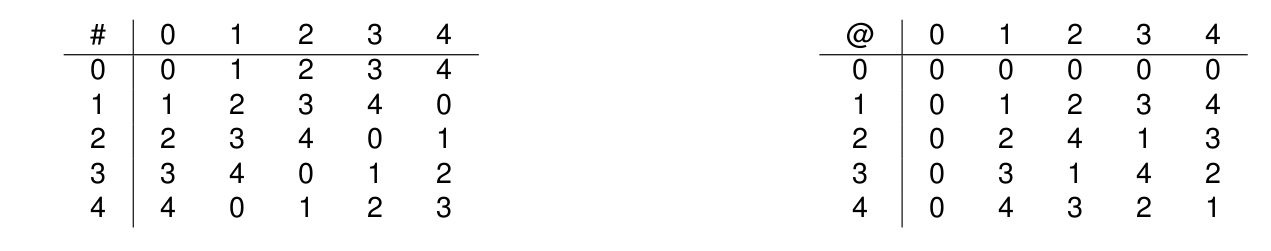
\includegraphics[width=10 cm]{2013_16.png}\newline


Com base nessas operações, considere as afirmativas a seguir.

I. A operação @ admite a propriedade comutativa.

II. A operação $\#$ admite a propriedade comutativa.

III. Na operação $\#$, 0 é o elemento neutro.

IV. Na operação @, 1 é o elemento inverso.

Assinale a alternativa correta.

a) Somente as afirmativas I e II são corretas.

b) Somente as afirmativas I e IV são corretas.

c) Somente as afirmativas III e IV são corretas.

d) Somente as afirmativas I, II e III são corretas.

e) Somente as afirmativas II, III e IV são corretas.\newline

\textbf{RESOLUÇÃO}

$\rule[1cm]{100cm}{1px}$

I. A operação @ admite a propriedade comutativa. (V)

II. A operação $\#$ admite a propriedade comutativa. (V)

III. Na operação $\#$, 0 é o elemento neutro. (V)

IV. Na operação @, 1 é o elemento inverso. (F)\newline

d) Somente as afirmativas I, II e III são corretas.\newline



\textbf{CONTEÚDO}

$\rule[1cm]{100cm}{1px}$

propriedades 

comutativa: para a propriedade ser válida temos que A.B = B.A 

elemento neutro: Propriedade do elemento neutro da adição é válida se somente se I+A=A 

\newpage

\item(2013, 19)Sobre o conjunto A = \{1, 2, 3, 4\}, considere as afirmativas a seguir.

I. P(a) = \{$\varnothing$, \{2, 3, 4\}\} é uma partição de A.

II. P(a) = \{$\varnothing$, \{1, 2, 3\}, \{3, 4\}\} é uma partição de A.

III. P(a) = \{\{1, 2\}, \{3, 4\}\} é uma partição de A.

IV. P(a) = \{\{1\}, \{2\}, \{3\}, \{4\}\} é uma partição de A.

Assinale a alternativa correta.

a) Somente as afirmativas I e II são corretas.

b) Somente as afirmativas I e IV são corretas.

c) Somente as afirmativas III e IV são corretas.

d) Somente as afirmativas I, II e III são corretas.

e) Somente as afirmativas II, III e IV são corretas.\newline

\textbf{RESOLUÇÃO}

$\rule[1cm]{100cm}{1px}$


I. P(a) = \{$\varnothing$, \{2, 3, 4\}\} é uma partição de A. (F)

II. P(a) = \{$\varnothing$, \{1, 2, 3\}, \{3, 4\}\} é uma partição de A. (F)

III. P(a) = \{\{1, 2\}, \{3, 4\}\} é uma partição de A. (V)

IV. P(a) = \{\{1\}, \{2\}, \{3\}, \{4\}\} é uma partição de A. (V)\newline

c) Somente as afirmativas III e IV são corretas.\newline



\textbf{CONTEÚDO}

$\rule[1cm]{100cm}{1px}$

$\{Ai: i \in I\}$ de um conjunto A é uma partição (sobre A) se cumpre-se que:

1: ${\displaystyle A_{i}\neq \emptyset }$ para todo ${\displaystyle i\in I} i \in I.$

2: ${\displaystyle \bigcup _{i\in I}A_{i}=A} $

3: ${\displaystyle A_{i}\cap A_{j}\neq \emptyset \Rightarrow A_{i}=A_{j}}$




\newpage






\item(2012, 15)Considere o circuito representado a seguir.

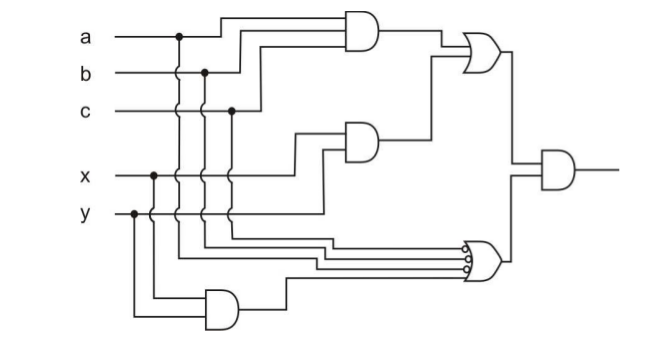
\includegraphics[width=10 cm]{2012_15.png}\newline

Assinale a alternativa que apresenta, corretamente, o circuito simplificado resultante.


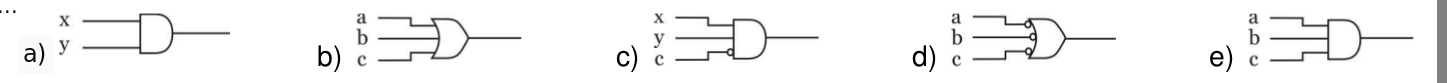
\includegraphics[width=10 cm]{2012_15_1.png}\newline

\textbf{RESOLUÇÃO}

$\rule[1cm]{100cm}{1px}$

$(((abc)+(xy)).((xy)+\lnot a + \lnot b + \lnot c))$

$((\lnot(abc).\lnot(xy))+(\lnot(xy)\lnot(\lnot a + \lnot b + \lnot c)))$

$(\lnot(xy)((\lnot(abc)+(\lnot(\lnot a + \lnot b + \lnot c)))) $

$(\lnot(xy)(\lnot(\lnot(abc)).\lnot(\lnot(\lnot a + \lnot b + \lnot c))) $

$((xy)+((\lnot(abc)+(\lnot(\lnot a + \lnot b + \lnot c))) $

$((xy)+(\lnot(abc).(abc))) $

$(xy)$\newline


a)x and y \newline

\textbf{CONTEÚDO}

$\rule[1cm]{100cm}{1px}$

a porta mais redonda representa a and ($\land$)

a porta mais mais pontuda representa a or ($\lor$)

o círcilo na prente da porta representa uma negação ($\lnot$)



\newpage


\item(2012, 16)Com relação à proposição P : “Seja $a \in N$. Se $a^2$ é ímpar então a é ímpar”, considere as afirmativas a seguir.

I. A proposição “Seja a $\in$ N. Se $a^2$ é par então a é par” tem o mesmo valor lógico da proposição P .

II. Redução ao absurdo da proposição P dada por “Seja a $\in$ N. Se  $a^2$ é ímpar ou a é par então tem-se
uma contradição” tem o mesmo valor lógico de P .

III. O contrapositivo da proposição P tem o mesmo valor lógico de P e é dado por “Seja a $\in$ N. Se a é
par então $a^2$ é par”.

IV. A recíproca da proposição P não tem o mesmo valor lógico de P e é dada por “Seja a $\in$ N. Se a é
ímpar então $a^2$ é ímpar”.

Assinale a alternativa correta.


a) Somente as afirmativas I e II são corretas.

b) Somente as afirmativas I e IV são corretas.

c) Somente as afirmativas III e IV são corretas.

d) Somente as afirmativas I, II e III são corretas.

e) Somente as afirmativas II, III e IV são corretas.\newline


\item(2012, 17)A tabela, a seguir, mostra as figuras geométricas e suas respectivas relações recursivas.


\includegraphics[width=10 cm]{2015.png}\newline


Nesta tabela podem ser observadas as seguintes relações:
T (1) = 1 para $F_3$ ; Q(2) = 4 para $F_4$ ; P (3) = 12 para $F_5$ ; H(4) = 28 para $F_6$ .

Com base na tabela e nas relações, assinale a alternativa que apresenta, corretamente, o número de
pontos de F 10 quando n = 5.

a) 55

b) 65

c) 75

d) 85

e) 95\newline





\item(2012, 18)Considerando os conjuntos A, B, C e D, assinale a alternativa que representa, corretamente, a região sombreada associada à relação $\{ (A\cap b)\cup (C\cap d) \}\cap \{ (A\cap b)\cup (B\cap c)\}$




\includegraphics[width=10 cm]{2015.png}\newline








\item(2012, 20)Considere a sentença, a seguir, com quantificadores que definem o limite de uma sequência ($a_n$).

$\forall \varepsilon > 0, \exists n 0 \in N, \forall n > n_0 , |a_n - L| < \in$

Assinale a alternativa que apresenta, corretamente, a negação dessa sentença

a) $\exists \varepsilon > 0, \exists n_0 \in N, \forall n < n_0 , |a_n - L| > \varepsilon$

b) $\exists \varepsilon > 0, \exists n_0 \in N,  \exists n > n_0 , |a_n - L| \geq \varepsilon$

c) $\exists \varepsilon < 0, \forall n_0 \in N, \exists n < n_0 , |a_n - L| > \varepsilon$

d) $\forall \varepsilon < 0, \forall n_0 \in N, \exists n > n_0 , |a_n - L| \geq \varepsilon$

e) $\exists \varepsilon > 0, \forall n_0 \in N, \exists n > n_0 , |a_n - L| \geq \varepsilon $\newline









\item(2011, 14)Considere as proposições p e q, cujas respectivas negações são $\bar p$ e $\bar q$. Então é correto afirmar que a recíproca de $p \rightarrow q$ é:

a) $\bar q \rightarrow \bar p$

b) $q \rightarrow p$

c) $\bar p \rightarrow \bar q$

d) $\bar p$ e $q$ 

e) $p$ e $\bar q$\newline

\textbf{RESOLUÇÃO}

$\rule[1cm]{100cm}{1px}$

1: $p \rightarrow q$ hip

2: $\bar p \lor q$ cond (1)

3:  $q \lor \bar p$ com(2)

4: $\bar q \rightarrow \bar p$ cond (3)\newline

a) $\bar q \rightarrow \bar p$\newline


\textbf{CONTEÚDO}

$\rule[1cm]{100cm}{1px}$

A recíproca é uma relação de implicação. Tendo-se duas proposições, A e B, há duas implicações que podem ser formadas usando estas propostas: Por exemplo: A recíproca de "Se ele ganhou na loteria então ele tem muito dinheiro", é "Se ele tem muito dinheiro então ele ganhou na loteria"

condicional(COND) $\phi \rightarrow \psi \equiv \sim \phi \vee \psi$


\newpage



\item(2011, 15)Considere o inteiro 360. Se x é a quantidade de seus divisores inteiros e positivos e y é a quantidade de seus divisores inteiros, positivos e pares, então é correto afirmar:

a) x divide y.

b) y divide x.

c) x = y.

d) x - y é múltiplo de 5.

e) x - y divide x e x - y divide y.\newline

\textbf{RESOLUÇÃO}

$\rule[1cm]{100cm}{1px}$

e) x - y divide x e x - y divide y.\newline



\textbf{CONTEÚDO}

$\rule[1cm]{100cm}{1px}$





\newpage







\item(2011, 16)Considere a afirmação a seguir.

Se um número inteiro é primo e quadrado perfeito, então ele é negativo.

Com relação a essa proposição, assinale a alternativa correta.

a) A afirmação é falsa.

b) A afirmação é verdadeira.

c) A afirmação é verdadeira e falsa.

d) Não é possível decidir se a afirmação é verdadeira ou falsa.

e) Não existe um inteiro primo negativo.\newline





\item(2011, 17)Sejam A e B eventos arbitrários de um espaço amostral, em que B é o complementar de B.
Nessas condições, é correto afirmar:

a) $P a) > P b)$

b) $P a) < P b)$

c) $P a) = P b)$

d) $P a) = P (\bar b)$

e) $P a) = P (A \cap b) + P (A \cap b)$\newline












\item(2010, 10) A relação de recorrência abaixo representa um processo de enumeração por recursão.

$
f(n) = \left \{ \begin{matrix} 

0, \hspace{70} \mbox{se } n=1\\
n T(n-1)+n \hspace{40} \mbox{se }  n>1
\end{matrix} \right.$ \newline

Assinale a alternativa que corresponde a um limite superior para o valor da fórmula fechada de tal relação
de recorrência.

a) T (1)

b) 0

c) $n^2$

d) 1024

e) n!\newline





\item(2010, 12) A deÆnição do Teorema Binomial de Newton é

$\hspace{60} (x+n)^2 = \sum_{i=0}^{n} (\frac{n}{i}) x^{n-i} y^i$

Assim, dado o seguinte somatório

 $\hspace{60} S_n  = \sum_{i=0}^{n} (\frac{n}{i})$

qual o valor de $S_n$ ?

a) n+1

b) $2^n -1$

c) (n-i)!

d) (n-1)!

e) $2(n^n -1)$4\newline






\item(2010, 14)Dada a proposição “existem números que são divisíveis por 3 e por 5 no conjunto”, assinale a alternativa em que essa proposição é verdadeira para um dos conjuntos a seguir.

a) \{2 , 8 , 9 , 20 , 135\}

b) \{9 , 20\}

c) \{18 , 55 , 67\}

d) \{2 , 3 , 5 , 7\}

e) \{9 , 18 , 36\}\newline

\textbf{RESOLUÇÃO}

$\rule[1cm]{100cm}{1px}$



a questão tenta lhe induzir ao erro fazendo você pensar que o conjunto tem que ter números que sejam diviziveis por 3 ou por 5 não os dois ao mesmo tempo 


a) \{2 , 8 , 9 , 20 , 135\}\newline



\textbf{CONTEÚDO}

$\rule[1cm]{100cm}{1px}$

o único número que é divisível por 3 e por 5 ao mesmo tempo e 135 que está no conjunto \{2 , 8 , 9 , 20 , 135\}

135/3=45

135/5=27



\newpage






\item(2010, 16)Os conectores lógicos $\lor$ , $→\rightarrow$ são lidos como “ou” e “implica”. O operador “não” é representado por $\lnot$ . Considerando esta notação, a tabela verdade da proposição $( P \rightarrow Q ) \rightarrow (\lnot Q \lor P )$ , assumindo que a sequência de valores de P é \{V,V,F,F\} e a de Q é \{V,F,V,F\}, tem os valores:

a) \{F,F,F,F\}

b) \{V,V,V,V\}

c) \{ V,V,F,V\}

d) \{F,F,V,V\}

e) \{V,F,V,F\}\newline





\item(2010, 17)A escala musical pode ser modelada matematicamente através da série harmônica. Usando a técnica de aproximação por integrais ou a de divisão por somatórios, um limite assintótico para a série harmônica

$H_m = \sum_{i=1}^n \frac{1}{i}$

é dado por:

a) $\log n+1$

b) dó, ré, mi, fá, sol, lá, si, dó

c) 3n + $\frac{1}{n}$

d) C,D,E,F,A,B

e) $ \frac{1}{i} + \frac{1}{i}+ ... + \frac{1}{i}  $ \newline



\item(2010, 20) Qual expressão matemática a seguir gera o n-ésimo termo da sequência 8+13+18+23+28+33+...?


a) $5n^2 + 3 n$

b) $3 + 5n$

c) $5( \frac{n^2 + n}{2} ) + 3n$

d) $8n + 5$

e) $2 ,5n^2 + 5 , 5n$



\item(2009, 3) Se $(x \mod{7} = 3)$ e $(x \mod{5} = 1)$, onde $x \geq 0$ , qual o menor valor inteiro possível para x?


a) 17

b) 25

c) 31

d) Existe um valor inteiro para x, que é diferente dos anteriores.

e) Não existe um valor inteiro para x.




\item(2009, 13) A sentença lógica $A\land (B\lor \lnot c)$

a) $A\land (\lnot B \land c)$

b) $\lnot A \land \lnot (B \lor \lnot c)$

c) $\lnot A \lor(\lnot B \land c)$

d) Todas as respostas anteriores.

e) Nenhuma das respostas anteriores.\newline





\item(2009, 14) Se é verdade que as três sentenças a seguir são verdade

$p \rightarrow q$

$r \rightarrow s$

$(p \land t ) \leftrightarrow r$

então é verdade que:

a) $\lnot s \rightarrow (t \lor p)$

b) $\lnot r \rightarrow \lnot s$

c) $\lnot q \rightarrow \lnot r$

d) Todas as respostas anteriores.

e) Nenhuma das respostas anteriores.\newline







\item(2009, 15)Existem três suspeitos de invadir uma rede de computadores: André, Bruna e Carlos.
Sabe-se que a invasão foi efetivamente cometida por um ou por mais de um deles, já
que podem ter agido individualmente ou não. Sabe-se, ainda, que:\newline

I. Se André é inocente, então Bruna é culpada.

II. Ou Carlos é culpado ou Bruna é culpada, mas não os dois.

III. Carlos não é inocente.\newline

Com base nestas considerações, conclui-se que:

a) Somente André é inocente.

b) Somente Bruna é culpada.

c) Somente Carlos é culpado.

d) São culpados apenas Bruna e Carlos.

e) São culpados apenas André e Carlos.\newline






\item(2009, 17) Considere os somatórios a seguir

I. $\sum_{i=1}^{\infty} \frac{1}{i}$

II. $\sum_{i=1}^{\infty} \frac{1}{i^2}$

III. $\sum_{i=1}^{\infty} a^i, 0< a <1$

IV. $\sum_{i=1}^{\infty} (-1)^i$

Assinale a alternativa CORRETA:

a) Apenas os somatórios I e II convergem.

b) Apenas os somatórios I e III convergem.

c) Apenas os somatórios II e III convergem.

d) Apenas os somatórios II e IV convergem.

e) Apenas os somatórios III e IV convergem.\newline





\item(2008, 63) Analise as seguintes afirmativas e assinale a alternativa CORRETA.

a) $ \varnothing \in \varnothing$

b) b) Se os conjuntos A , B e C são tais que $ A \cup B = A \cup C$ e $A \cap B = A \cap c$= então $B \ne C B = C$

c) A sentença $(P \rightarrow \lnot Q) \lor P$ tem valor V quaisquer que sejam os valores atribuídos a P e Q .

d) Todas as afirmativas anteriores são verdadeiras.

e) Todas as afirmativas anteriores são falsas.\newline


\item(2008, 64) Considere as seguintes afirmações:

I. Se $R \cap R^{-1}$ é uma relação de equivalência, então R é uma relação reflexiva e transitiva. 

II. Se F e G são duas funções inversíveis, então $G \circ F$ é uma função inversível.

III. Sejam $K \in N$ e $A \subset N$. Se $ K \in A $ e $(n \in A, n \geq k \rightarrow n+1 \in a)$ então $ A=N$

IV. Para todo conjunto A, $\xia)$ denota o conjunto de todos os subconjuntos de A . A relação \{$(a,a'):a\in \xia), a' \in \xia), a \subseteq a' $

Assinale a quantidade de afirmativas CORRETAS.

a) 0

b) 1

c) 2

d) 3

e) 4\newline



\item(2008, 65) Defina os conectivos NIMP, NEQ, NAND, negação da implicação, equivalência e conjunção, respectivamente, como:

$(\alpha NIMP \beta) \equiv \lnot(\alpha \rightarrow \beta)$

$(\alpha NEQ \beta) \equiv \lnot(\alpha \leftrightarrow \beta)$

$(\alpha NAND \beta) \equiv \lnot(\alpha \land \beta)$

Assinale alternativa que representa um conjunto de conectivos completo.

a) \{ NIMP \}

b) \{ NEQ \}

c) \{ NAND \}

d) \{ NIMP , NEQ \}

e) Nenhum é completo\newline




\item(2008, 66) Analise as seguintes afirmativas e assinale a alternativa INCORRETA.

a) $1 + 2 + 2^2 + 2^3 + ... + 2^n = 2^{n+1} - 1 , para todo$ $n \in N$

b)$C_p^{n+p+1} =\sum_{r=0}^p$ $C_r^{n+r}$ , para todo $n \in N$ e $p \in N$  

c) Para todo conjunto $A , \xia)$ denota o conjunto de todos os subconjuntos de A . Se $A \subseteq B $ então $\xia)  \subseteq  \xib)$

d) $Se A_1 , A_2 ,..., A_r$ são conjuntos disjuntos, então $|A_1\cup A_2\cup ...\cup A_r\cup B|<|B|+\sum_{i=1}^{r}(|A_i -B|)$

e) Se a afirmativa a) é falsa, então a afirmativa d) é falsa.\newline





\item(2008, 67) Em relação ao conjunto parcialmente ordenado A (\{ a , b , c , d , e , f \},$\leq$ ) , representado pelo diagrama de Hasse abaixo, analise as seguintes afirmativas.

I. A estrutura A não é reticulado.

II. Os majorantes de { b , c } são os elementos d e e .

III. O ínfimo de { d , e } é o elemento a .

IV. A estrutura é um reticulado limitado com topo sendo o elemento a e o fundo f.

V. A estrutura A possui apenas dois subconjuntos de 4 elementos totalmente ordenados:
\{ a , b , d , f \} e \{ a , c , e , f \} .

\includegraphics[width=10 cm]{2015.png}\newline

A análise permite concluir que

a) somente III e IV são falsas.

b) somente I e II são falsas.

c) somente V é falsa.

d) somente IV é verdadeira.

e) somente I é verdade\newline



\item(2008, 68)Analise as seguintes relações sobre o conjunto A {1, 2,3} :

R {(2,1), (3,1), (3,3)} , S{(1,1), (2,2)} , T{(1,2), (1,3)} e U{(2,3), (3, 2)} .\newline

I. Somente S é reflexiva.

II. Somente U não é transitivas.

III. Somente U é simétrica.

IV. Nenhuma delas é antissimétrica.

V. $R\cup S$ é reflexiva, antissimétrica e transitiva.

VI. $S\cup U$ não é reflexiva, mas é transitiva e simétrica.

VII. $R\cup S\cup T$ é reflexiva e simétrica, mas não é transitiva.

A análise permite concluir que são VERDADEIRAS \newline

a) somente as afirmativas II, V e VI.

b) somente as afirmativas I, II, e VII.

c) somente as afirmativas III, V e IV.

d) somente as afirmativas I, III, VI, VII.

e) todas as afirmativas.\newline





\item(2008, 69)Sobre o conjunto X=\{A,B,C,D,E\}, em que A \{$\varnothing$\}, B=\{a,b\}, C=\{b,c\}, B=\{a,b,c\} e F=\{a,b,c,d\}, fazem-se as seguintes afirmativas:\newline

I. X é fechado para a operação de união de conjuntos.

II. X é fechado para a operação de interseção de conjuntos.

III. X não é fechado para a operação de complementação de conjuntos.

IV. (X, $\cup$) , em que $\cup$ é a operação de união de conjuntos, é um monóide não comutativo.

V. (X, $\cap$ ) , em que $\cap$ é a operação de interseção de conjuntos, não é um monóide, porque X não apresenta elemento neutro para $\cap$.\newline

São CORRETAS\newline

a) apenas as afirmativas I, II e III.

b) apenas as afirmativas I e IV.

c) apenas as afirmativas II e V.

d) apenas as afirmativas I e III.

e) todas as afirmativas.\newline





\item(2007, 10)Dados os conceitos de coerência e completeza de um sistema dedutivo, analise
as seguintes afirmativas.

I. Existe pelo menos um sistema de dedução coerente e completo para a Lógica Proposicional.

II. Todo sistema de dedução para a Lógica de Predicados de Primeira Ordem que é completo também é coerente.

III. Existe pelo menos um sistema de dedução coerente e completo para a Lógica de Predicados de Primeira Ordem.

A partir da análise, pode-se concluir que é(são) VERDADEIRA(S)

a) nenhuma das afirmativas.

b) somente as afirmativas I e II.

c) somente as afirmativas I e III.

d) somente as afirmativas II e III.

e) todas as afirmativas.\newline



\item(2007, 11)Considere a seguinte linguagem de primeira ordem:

• constantes: a, b

• variáveis: x, y

• predicados unários: P

• predicados binários: R

Considere a seguinte função de interpretação $I$ para essa linguagem, com valores no
conjunto $N$ dos números naturais:

• $Ia) = Ib) = 0$

• $I(P ) = \{n | n < 4\}$

• $I(R) = \{(x, y) | x < y\}$\\

Dadas as seguintes fórmulas:\\

I. $P a)$

II. $\forall x, y : R(x, y) \rightarrow R(y, x)$

III. $\exists x : R(x, a)$\\

Em relação à função de interpretação I definida acima, pode-se afirmar que é(são) VERDADEIRA(AS)

a) somente a fórmula I.

b) somente as fórmulas I e II.

c) somente a fórmula III.

d) nenhuma das fórmulas.

e) todas as fórmulas.\newline



\item(2007, 12)Seja * um conectivo ternário definido por: *($\alpha, \beta, \gamma$) é verdadeiro se, e somente se, ou nenhuma ou apenas uma das fórmulas $\alpha, \beta, \gamma$ é verdadeira.

Assinale a alternativa que apresenta a fórmula equivalente a  *($\alpha, \beta, \gamma$).

a) $(\alpha \vee \beta \vee \gamma) \wedge(\alpha \vee(\neg \beta) \vee(\neg \gamma)) \wedge((\neg \alpha) \vee \beta \vee(\neg \gamma)) \wedge((\neg \alpha) \vee(\neg \beta) \vee \gamma)$

b) $((\neg \alpha) \wedge(\neg \beta) \wedge(\neg \gamma)) \vee(\alpha \wedge(\neg \beta) \wedge(\neg \gamma)) \vee((\neg \alpha) \wedge \beta \wedge(\neg \gamma)) \vee((\neg \alpha) \wedge(\neg(\neg \beta)) \wedge \gamma)$

c) $(\alpha \vee(\neg \beta) \vee(\neg \gamma)) \wedge((\neg \alpha) \vee \beta \vee(\neg \gamma)) \wedge((\neg \alpha) \vee(\neg \beta) \vee \gamma)$

d) $((\neg \alpha) \wedge(\neg \beta) \wedge(\neg \gamma)) \vee(\alpha \wedge(\neg \beta) \wedge(\neg \gamma)) \vee((\neg \alpha) \wedge \beta \wedge(\neg \gamma)) \vee((\neg \alpha) \wedge(\neg \beta) \wedge \gamma)$

e) Nenhuma destas respostas é correta.\newline


\item(2007, 13) Um conjunto C, subconjunto de um conjunto A, é decidı́vel se existe um programa que recebe uma entrada $x \in A$, e sempre pára indicando se $x \in C$ ou se $x \notin C$.

Entre os conjuntos relacionados abaixo, assinale o que NÃO é decidı́vel.

a) O conjunto das fórmulas satisfatı́veis da lógica clássica proposicional.

b) O conjunto dos teoremas da lógica clássica proposicional.

c) O conjunto dos teoremas da lógica clássica de primeira ordem.

d) O conjunto das fórmulas da lógica clássica de primeira ordem.

e) O conjunto das tautologias da lógica clássica proposicional.\newline


\item(2007, 14) Analise as seguintes afirmativas e assinale a alternativa CORRETA.

a) $\{\{ \not 0 \}\} \in \{ \not 0,\{\not 0 \}\}$

b)Para todo conjunto A, Pa) denota o conjunto de todos os subconjuntos de A. Se a e B são conjuntos tais que $a \in B$, então $Pa) \subseteq Pb)$

c) O conjunto $\{n 109 : n ∈ N\}$ é infinito enumerável.

d) Se A, B e C são três conjuntos, então $A − (B - c) = (A - b) - C.$

e) Nenhuma das afirmativas anteriores é correta.\newline



\item(2007, 15) Analise as seguintes alternativas e assinale a que apresenta uma afirmativa FALSA.

a) Se $A_{1}, A_{2}, \cdots, A_{r}$ sâo conjuntos disjuntos, então $\left|A_{1} \cup \cdots \cup A_{r} \cup B\right|=|B|+$
$\sum_{i=1}^{r}\left(\left|A_{i}-B\right|\right) .$

b) $1+2+2^{2}+2^{3}+\cdots+2^{n}=2^{n+1}-1,$ para todo $n \in \mathbb{N}$

c) $C_{p}^{n+p+1}=\sum_{r=0}^{p} C_{r}^{n+r},$ para todo $n \in \mathbb{N}$ e $p \in \mathbb{N}$

d) Sejam $k \in \mathbb{N}$ e $A \subseteq \mathbb{N} .$ Se $k \in A$ e $(n \in A, n \geq k \Rightarrow n+1 \in a),$ então 
\tildeo $A=\mathbb{N}$

e) Existe exatamente uma alternativa falsa dentre as anterio\newline




\item(2007, 16) Analise as seguintes afirmativas.

I. Seja A = P(X) o conjunto dos subconjuntos de um conjunto X. A relação

$\preceq=\left\{\left(a, a^{\prime}\right) : a \in A, a^{\prime} \in A, a \subseteq a^{\prime}\right\}$
é uma relação de ordem parcial.

II. Se $R$ é uma relaçâo binária simétrica e anti-simétrica, então \tildeo $R=\emptyset$

III. Seja $R$ uma relação reflexiva em um conjunto A. Então, $R$ é uma relação de equivalência se e somente se $((a, b) \in R \mathrm{e}(b, c) \in R \Rightarrow(c, a) \in R)$

IV. Se F e G são duas funções inversı́veis, então G ◦ F é uma função inversı́vel.

Assinale a alternativa que apresenta a quantidade de afirmativas CORRETAS.\newline

a) 0 (zero)

b) 1 (uma)

c) 2 (duas)

d) 3 (três)

e) 4 (quatro)\newline



\item(2007, 17) Sejam R e S relações em um conjunto A o qual contém pelo menos três elementos.
Analise as seguintes afirmativas.

I. Se R e S são simétricas, então R $\cap$ S é simétrica.

II. Se R e S são simétricas, então R $\cup$ S é simétrica.

III. Se R e S são reflexivas, então R $\cap$ S é reflexiva.

IV. Se R e S são reflexivas, então R $\cup$ S é reflexiva.\\

A análise permite concluir que está(ão) CORRETA(AS)\\

a) apenas a afirmativa I.

b) apenas as afirmativas I e II.

c) apenas as afirmativas II e IV.

d) apenas as afirmativas III e IV.

e) todas as afirmativas.\newline





\item(2006, 9) Assinale a proposição logicamente equivalente a $\neg(p \vee q) \vee(\neg p \wedge q)$

a) $\neg p \wedge(q \vee \neg q)$

b) $\neg p$

c) $(p \vee q) \wedge(p \vee \neg q)$

d) $(p \vee q) \vee(p \wedge \neg q)$

e) $p$ \newline
    



\item(2006, 10) Considere as seguintes proposições:

(I) $\neg p \vee q$

(II) $\neg(p \wedge \neg q)$

(III) $p \longrightarrow q$

(IV) $(V \longrightarrow q) \vee(p \longrightarrow F)$
    
Quais das proposições acima são logicamente equivalentes ?    

a) Somente $(\mathrm{I}) \equiv(\mathrm{III})$

b) Somente $(\mathrm{I}) \equiv(\mathrm{II})$

c) Somente $(\mathrm{I}) \equiv(\mathrm{II}) \equiv(\mathrm{III})$

d) $(\mathrm{I}) \equiv(\mathrm{III}) \mathrm{e}(\mathrm{II}) \equiv(\mathrm{III}) \mathrm{mas}(\mathrm{III}) \not \equiv(\mathrm{IV})$

e) $(\mathrm{I}),(\mathrm{II}),(\mathrm{III}) \mathrm{e}(\mathrm{IV})$ sâo todas equivalentes.\newline




\item(2006, 12) Seja o conjunto $A=\{x \in \mathbb{R},|x| \geq 1\}$ Qual das alternativas é uma partição do
conjunto A.

a) $\{x<-1\},\{x>1\},\{1,-1\}$

b) $\{x \leq 0\},\{x \geq 1\},\{0\}$

c) $\{x \leq-1\},\{x \geq 3\},\{1 \leq x \leq 3\}$

d) $\{x \leq-5\},\{-5<x \leq-3\},\{-1\},\{x \geq 1\}$

e) Todas as alternativas são partições de A.




\item(2005, 12) Determine qual das seguintes proposições não pode ser provada a partir da premissa:

$$((a \wedge b) \vee c) \wedge(c \rightarrow d)$$

a) $(a \vee d) \wedge(b \vee d)$

b) $(\neg a \vee \neg b) \rightarrow(c \wedge d)$

c) $(a \wedge b) \rightarrow \neg d$

d) $\neg a \rightarrow d$

e) $\neg d \rightarrow b$ \newline



\item(2005, 13) Dadas as quatro premissas:

• Se o universo é finito, então a vida é curta.

• Se a vida vale a pena, então a vida é complexa.

• Se a vida é curta ou complexa, então a vida tem sentido.

• A vida não tem sentido.

e as assertivas lógicas:

(I) se o universo é finito e a vida vale a pena, então a vida tem sentido;

(II) a vida não é curta;

(III) a vida tem sentido ou o universo é finito;

quais assertivas pode-se dizer que se seguem logicamente das premissas dadas?

a) Somente (I) e (III)

b) Somente (II) e (III)

c) Somente (I) e (II)

d) (I), (II) e (III)

e) Somente a assertiva (I).\newline


\item(2005, 14) Considere a seguinte proposição: 

$$P : \forall x[B x \rightarrow[L x \wedge C x]]$$

Assinale a alternativa que contém uma proposição equivalente a $\neg P$

a) $\forall x \neg[B x \rightarrow[L x \wedge C x]]$

b) $\exists x[B x \wedge[\neg L x \vee \neg C x]]$

c) $\forall x[B x \rightarrow \neg[L x \wedge C x]] .$

d) $\exists x[\neg B x \wedge[\neg L x \vee \neg C x]] .$

e) $\exists x[\neg B x \vee[L x \wedge C x]]$ \newline





\item(2005, 16) Sejam a, b e n inteiros, com $n>0$ Considere a equação:

$$a x \equiv b \quad(\bmod n)$$


a) A equação acima não tem solução.

b) A equação acima sempre tem solução.

c) A equação acima tem solução se mdc(a, n) = 1.

d) A equação acima tem solução se mdc(a, b) = 1.

e) A equação acima tem solução se mdc(b, n) = 1.\newline






\item(2005, 18) Dadas as seguintes afirmações:

(I) se R é uma relação transitiva, a sua inversa também é transitiva.

(II) se R é uma relação reflexiva, anti-simétrica e transitiva, então a sua inversa
também é uma relação reflexiva, anti-simétrica e transitiva.

(III) se R é uma relação simétrica e transitiva, então R é reflexiva.

São verdadeiras:

a) Somente (I) e (II)

b) Somente (II) e (III)

c) Somente (I) e (III)

d) (I), (II) e (III)

e) Somente (I) é verdadeira. \newline






\item(2004, 10) Quais são as raı́zes da equação caracterı́stica da relação de recorrência: 

$$\left\{\begin{array}{l}{a_{1}=0} \\ {a_{2}=1} \\ {a_{n}=-a_{n-2} \quad(n \geq 3)}\end{array}\right.$$

a) $0,1$ e $-1$

b) $i, 0$ e $-i$

c) $i$ e $-i$

d) 0 e 1

e) 0 e $-1$


\item(2004, 11) A sequência definida recursivamente por

$$T_{n}=n+1+\frac{2}{n} \sum_{k=0}^{n-1} T_{k} \quad\left(\forall n>0 ; T_{0}=0\right)$$

pode ser definida por uma expressão na forma $a_{n} T_{n}=b_{n} T_{n-1}+c_{n}$ Neste caso, quais
são os valores de $a_{n}, b_{n}$ e $c_{n}$?

a) $n, 1$ e $\frac{n}{2} \sum_{k=0}^{n-2} T_{k}$

b) $n,(n+1)$ e 2$n$

c) $n, 1$ e 2$n \sum_{k=0}^{n-2} T_{k}$

d) $n,(n+1)$ e $\frac{2}{n}$

e) $n, 1$ e $\frac{2}{n} \sum_{k=0}^{n-2} T_{k}$\newline







\item(2004, 20) Considere a fórmula e o domı́nio de interpretação a seguir:

$$[\forall x[F x \Rightarrow[E x \wedge T x a]]] \wedge$$
$$[\exists x[[E x \wedge T x a] \wedge F x]] \wedge$$
$$[\exists x[[E x \wedge T x] \wedge \neg F x]]$$

Domı́nio: Universo

a: Alberto

Ex: x é estudante

F x: x formou-se

T xy: x trabalhou mais que y

Qual sentença é logicamente consistente com a fórmula usando o domı́nio de interpretação apresentado?

a) Todos os estudantes que trabalharam mais que Alberto formaram-se.

b) Somente estudantes que trabalharam mais que Alberto formaram-se.

c) Alberto trabalhou mais que qualquer estudante que não se formou.

d) Somente estudantes que se formaram trabalharam mais que Alberto.

e) Todos os estudantes que não se formaram trabalharam menos que Alberto.\newline







\item(2003, 15) Sejam $f : S \rightarrow T$ uma função, $A, B \subset S$ e $U, V \subset T .$ é correto afirmar que

a) $f(A \cap b)=fa) \cap fb)$

b) $f^{-1}(U \cap V)=f^{-1}(U) \cap f^{-1}(V)$

c) $f^{-1}(fa))=A$

d) $f(A \backslash b)=fa) \backslash fb)$

e) $f\left(f^{-1}(U)\right)=U$ \newline

\item(2003, 16)Assinale a forma correta da negação da seguinte frase:

”Algumas pessoas gostam de matemática .”

a) Algumas pessoas não gostam de matemática.

b) Todas as pessoas não gostam de matemática.

c) Existe uma pessoa que gosta de matemática.

d) Existe uma pessoa que não gosta de matemática.

e) Todas as pessoas gostam de matemática. \newline




\item(2003, 17) Assinale o argumento válido, onde $S_1$ e $S_2$ indicam premissas e C a conclusão.

a)

$S 1$ : Se a comida é boa, então o serviço é bom.

$S 2$ : A comida não é boa.

$C$: O serviço não é bom.\\

b)

$S 1$ : Se a comida é boa, então o serviço é bom.

$S 2$: O serviço não é bom.

$C$: A comida é boa.\\

c)

$S 1$ : Se a comida é boa, então o serviço é bom.

$S 2$ : O serviço não é bom.

$C$: A comida não é boa.\\

d)

$S 1$ : Se a comida é boa, então o serviço é bom.

$S 2$ : A comida é boa.

$C$: O serviço não é bom.\\

e)

$S 1$ : Se a comida é boa, então o serviço é bom.

$S 2$ : A comida não é boa.

$C$: O serviço é bom.\newline


\item(2002, 3) a n um número inteiro positivo. Considere a função f definida recursivamente por

$$f(n)=\left\{\begin{array}{cc}{0} & {\text { se } n=1} \\ {f\left(\left\lfloor\frac{n}{2}\right\rfloor\right)+1} & {\text { se } n>1}\end{array}\right.$$

onde $\lfloor k\rfloor$ é o maior inteiro menor ou igual a $k$ . O valor de $f(25)$ é igual a

a) 5

b) 4

c) 6

d) 3

e) 2 \newline

\textbf{RESOLUÇÃO}

$\rule[1cm]{100cm}{1px}$

$\begin{aligned} f(25) &=f\left(\left\lfloor\frac{25}{2}\right\rfloor\right)+1 \\ &=f(12)+1 \\ &=f\left(\left\lfloor\frac{12}{2}\right\rfloor\right)+1+1 \\ &=f(6)+1+1 \\ &\left.=f\left(\frac{6}{2}\right\rfloor\right)+1+1+1 \\ &=f(1)+1+1+1 \\ &=0+1+1+1+1 \\ &=4 \end{aligned}$


\textbf{CONTEÚDO}

$\rule[1cm]{100cm}{1px}$

temos que uma função recursiva executará até chegar em seu caso base que no caso será n = 1, e o  resultado de f(n) enquanto for diferente de 1 ele chamará novamente a função 

\newpage





\item(2002, 10) Assinale o argumento válido, onde $S_{1}, S_{2}$ indicam premissas e $S$ a conclusâo:

a)

$S_1$ : Se o cavalo estiver cansado então ele perderá a corrida

$S_2$ : O cavalo estava descansado

$S$: O cavalo ganhou a corrida\\

b) 

$S_1$ : Se o cavalo estiver cansado então ele perderá a corrida

$S_2$ : O cavalo ganhou a corrida

$S$: O cavalo estava descansado\\

c) 

$S_1$ : Se o cavalo estiver cansado então ele perderá a corrida

$S_2$ : O cavalo perdeu a corrida

$S$: O cavalo estava cansado\\

d) 

$S_1$ : Se o cavalo estiver cansado então ele perderá a corrida

$S_2$ : O cavalo estava descansado

$S$: O cavalo perdeu a corrida\\

e) nenhuma das anteriores \newline


\textbf{RESOLUÇÃO}

$\rule[1cm]{100cm}{1px}$

$$
\begin{array}{l}{\bullet \mathrm{p} : \text { cavalo cansado }} \\ {\bullet \mathrm{q} : \text { ganhar a corrida }}\end{array}
$$

$$
\begin{array}{l}{S_{1} \wedge S_{2} \rightarrow S=(p \rightarrow \neg q) \wedge q \rightarrow \neg p} \\ {S_{1} \wedge S_{2} \rightarrow S=(\neg p \vee \neg q) \wedge q \rightarrow \neg p} \\ {S_{1} \wedge S_{2} \rightarrow S=(\neg p \wedge q) \vee(\neg q \wedge q) \rightarrow \neg p} \\ {S_{1} \wedge S_{2} \rightarrow S=(\neg p \wedge q) \vee F A L S 0 \rightarrow \neg p} \\ {S_{1} \wedge S_{2} \rightarrow S=(\neg p \wedge q) \vee F A L S 0 \rightarrow \neg p} \\ {S_{1} \wedge S_{2} \rightarrow S=(\neg p \wedge q) \rightarrow \neg p} \\ {S_{1} \wedge S_{2} \rightarrow S=p \vee \neg q \vee r p} \\ {S_{1} \wedge S_{2} \rightarrow S=p \vee \neg p \vee \neg q} \\ {S_{1} \wedge S_{2} \rightarrow S=V E R D A D E I R 0 \quad \vee \neg q} \\ {S_{1} \wedge S_{2} \rightarrow S=V E R D A D E I R 0}\end{array}
$$\newline

b)\newline


\textbf{CONTEÚDO}

$\rule[1cm]{100cm}{1px}$





\newpage






\item(2002, 20) Três atletas A, B e C competiram, ao pares, numa corrida de d metros. Considerando que cada atleta teve o mesmo desempenho (ou seja, a mesma velocidade) ao competir com adversários distintos, e sabendo-se que

• A venceu B chegando 20 metros à frente

• B venceu C chegando 10 metros à frente

• A venceu C chegando 28 metros à frente,

podemos afirmar que a corrida tem

a) 50 metros

b) 200 metros

c) 100 metros

d) 150 metros

e) 110 metros \newline




















\end{enumerate}

\newpage
\section{ÁLGEBRA}\\
\begin{enumerate}


\item (2018, 1) Para quais valores de a, b, c, d, e, f a matriz J =
$\Bigg(
    \begin{array}{cccc}
    3 & 0 & 0 & 0 \\
    a & 2 & d & e \\
    b & 0 & 1 & 0 \\
    c & 0 & f & 0 \\
\end{array}\Bigg)$ é diagonalizável?\newline

\noindent a) Não pode ser diagonalizável.

b) Apenas para números inteiros.

c) Somente para números positivos.

 d) Para quaisquer valores.

e) Somente para valores nulos.\newline

\textbf{RESOLUÇÃO}

$\rule[1cm]{100cm}{1px}$



\textbf{CONTEÚDO}

$\rule[1cm]{100cm}{1px}$

diagonalizável: uma condição suficiente para que uma matriz de ordem n seja diagonalizável e que ela possua n aulovalores distintos 

polinômio caracteristico e os auto valores são os zeros desse polinômio 



\newpage



\item (2018, 2)Calcule as coordenadas de $1 + t + t^2$ na base $(1, t-1, (t -1)^2 )$ , considerando $E =
R_2 [t]$, sendo as coordenadas: $(\lambda, \mu, \eta)$.\newline

a) η = 1, μ = 3, λ = 3

b) η = 0, μ = 3, λ = 3

c) η = −1, μ = 1, λ = 1

d) η = 1, μ = 2, λ = 1

e) η = 3, μ = 3, λ = 3\newline



\item (2018, 3) O vetor diretor de uma reta r é $\vec v =(-1,2)$ e passa pelo ponto P(-5, -5). A outra
reta s tem pendente m=-2 e passa pelo ponto N(0, 5). Em relação à disposição das retas, elas:\newline

a) São perpendiculares.

b) São paralelas.

c) Se cruzam.

d) São tangentes.

ae) Não são retas.\newline


\textbf{RESOLUÇÃO}

$\rule[1cm]{100cm}{1px}$



\textbf{CONTEÚDO}

$\rule[1cm]{100cm}{1px}$

pendente e o mesmo que coeficiente angular 

vetor diretor e o vetor não nulo que tem a mesma direção da reta


\newpage




\item (2018, 4) Dados os vetores $\vec u = (5,4)$ e $\vec v = (−3,$2) , calcule o produto escalar e o ângulo que elas formam entre si:\newline

a) 7; 107°

b) 7; -107°

c) -7; 72°

d) 7; 72°

e) -7; 107°\newline
\textbf{RESOLUÇÃO}

$\rule[1cm]{100cm}{1px}$

PPRODUTO ESCALAR:

$5.(-3)+4.2$

$-15+8=-7$\newline

ÂNGULO:

$\vec u .\vec v=\cos{\theta}.|u|.|v|$

$\cos{\theta}=\frac{-7}{\sqrt{5^2 + 4^2}.\sqrt{(-3)^2 + 2^2}}$

$\cos{\theta}=\frac{-7}{\sqrt{553}}$\newline

como o $\cos{\theta}$ e negativo temos que o ângulo só pode estar no segundo quadrane e analisando as alternativas a única opção seroa 107\newline

e) -7; 107°\newline

\textbf{CONTEÚDO}

$\rule[1cm]{100cm}{1px}$

ÂNGULO ENTRE DOIS VETORES:
Através da definição de produto escalar, podemos obter o ângulo x entre dois vetores genéricos u e v:

$\vec u .\vec v=\cos{\theta}.|u|.|v|$


\newpage




\item (2018, 7) Determine a matriz inversa de A= $\frac{1}{13} \Bigg(
    \begin{array}{cccc}
    1 & 3 & 5\\
    0 & -1 & 4\\
    1 & 1 & 0 \\
\end{array}\Bigg):$\newline

a) $A^{-1}=\frac{1}{13} \Bigg(
    \begin{array}{cccc}
    1 & 0 & 1\\
    3 & -1 & 1\\
    5 & 4 & 0 \\
\end{array}\Bigg)$\\

b)$A^{-1}= \Bigg(
    \begin{array}{cccc}
    1 & 3 & 5\\
    0 & -1 & 4\\
    1 & 1 & 0 \\
\end{array}\Bigg)$\\

c)$A^{-1}=\Bigg(
    \begin{array}{cccc}
    -4 & 5 & 17\\
    4 & -5 & -4\\
    1 & 2 & -1 \\
\end{array}\Bigg)$\\

d)$A^{-1}=\frac{1}{13} \Bigg(
    \begin{array}{cccc}
    -4 & 5 & 17\\
    4 & -5 & -4\\
    1 & 2  & -1\\
\end{array}\Bigg)$\\

e)$A^{-1}=\Bigg(
    \begin{array}{cccc}
    -5 & 3 & 12\\
    0 & -1 & 4 \\
    -1 & 1 & -4 \\
\end{array}\Bigg)$\\

\textbf{RESOLUÇÃO}

$\rule[1cm]{100cm}{1px}$

$(\frac{1}{DET }$.mat cof A)^t$

A= $\frac{1}{13} \Bigg(
    \begin{array}{ccc}
    \frac{1}{13} & \frac{3}{13} & \frac{5}{13}\\
    0 & \frac{-1}{13} & \frac{4}{13}\\
    \frac{1}{13} & \frac{1}{13} & 0 \\
\end{array}\Bigg)$

$DET=(\frac{12}{13^2}+0+0)$ - $(0 -\frac{5}{13^2}+\frac{4}{13^2})$

$DET=\frac{1}{169}$\newline

aplicando a matriz dos cofatores\newline

A= $\Bigg(
    \begin{array}{ccc}
    -\frac{4}{169} & +\frac{+4}{169} & +\frac{1}{169}\\
    +\frac{-5}{169} & -\frac{5}{169} & +\frac{2}{169}\\
    +\frac{17}{169} & -\frac{4}{169} & -\frac{1}{169} \\
\end{array}\Bigg).\frac{1}{\frac{1}{169}}$\newline

A= $\Bigg(
    \begin{array}{ccc}
    -\frac{4}{\not{169}} & +\frac{+4}{\not{169}} & +\frac{1}{\not{169}}\\
    +\frac{5}{\not{169}} & -\frac{5}{\not{169}} & +\frac{2}{\not{169}}\\
    +\frac{17}{\not{169}} & -\frac{4}{\not{169}} & -\frac{1}{\not{169}} \\
\end{array}\Bigg).\not{169}$\newline

A= $\Bigg(
    \begin{array}{ccc}
    -4  & 4 & 1\\
    5 & 5 & 2\\
    17 & 4 & 1\\
\end{array}\Bigg)$\newline

A= $\Bigg(
    \begin{array}{ccc}
    -4  & 5 & 17\\
    4 & -5 &  -4\\
    1 & 2 & -1\\
\end{array}\Bigg)$\newline

c)$A^{-1}=\Bigg(
    \begin{array}{cccc}
    -4 & 5 & 17\\
    4 & -5 & -4\\
    1 & 2 & -1 \\
\end{array}\Bigg)$\\\newline



\textbf{CONTEÚDO}

$\rule[1cm]{100cm}{1px}$

(1 / sobre a matriz determinante A . matriz dos cofatores A)$^{transposta}$

COFATOR:$A_{ij}=(-1)^{i+j}.D_{ij}$

Devemos compreender os elementos dessa expressão. O valor $A_{ij}$ é justamente o cofator do elemento aij da matriz A, enquanto que $D_{ij}$ será o determinante da matriz obtida através da matriz A, entretanto você deverá excluir da matriz A os elementos da linha i e da coluna j. Façamos um exemplo para melhor compreensão dessa expressão do cofator.\newline

TRANSPOSTA:Determinar a transposta de uma matriz é reescrevê-la de forma que suas linhas e colunas troquem de posições ordenadamente, isto é, a primeira linha é reescrita como a primeira coluna, a segunda linha é reescrita como a segunda coluna e assim por diante, até que se termine de reescrever todas as linhas na forma de coluna.




\newpage





\item (2017, 1) Sendo F = [(1,1,-1)], a projeção ortogonal de (2,4,1) sobre o subespaço ortogonal
de F é:

a) (1,2,3)

b) (1/3, 7/3, 8/3)

c) (1/3, 2/3, 8/3)

d) (0, 0, 0)

e) (1, 1, 1)\newline



\item (2017, 2) Qual é o valor do determinante da matriz 5x5
$\Bigg(
    \begin{array}{ccccc}
    1 & 2 & 3 & 4 & 5 \\
    4 & 3 & 4 & 0 & 0 \\
    8 & 6 & 7 & 2 & 0 \\
    12 & 9 & 10 & 3 & 0 \\
    16 & 12 & 13 & 4 & 0 \\
\end{array}\Bigg)$?

a) 325

b) 5

c) 120

d) 1

e) 0\newline




\item (2017, 3) Em um espaço $R^3$ , as retas: $r \equiv \frac{x+5}{4} = \frac{y-3}{-2} = \frac{z+4}{3}$ e  $s \equiv (x,y,z) = (1,1,-2) + [(1,-1,2)]$:\newline

a) São ortogonais.

b) Não são ortogonais e são contidas em um plano.

c) Não têm pontos em comum.

d) São paralelas.

e) Não são retas.\newline







\item (2017, 10) Sendo u(x,y),v(x,y) as funções implícitas definidas pelo sistema 
$\left \{ \begin{matrix}
xe^u + yu =1\\
2x^2v + y^3 e^u =1
\end{matrix} \right.$

localmente no ponto $(x_0 , y_0 , u_0 , v_0 ) $= (1,1,0,0) , assinale a matriz da diferencial de (u(x, y), v(x, y))no ponto (1,1).


a) 
$\Bigg(
    \begin{array}{cc}
    1/2 & 1 \\
    1/2 & 2 \\
\end{array}\Bigg)$

b)
$\Bigg(
    \begin{array}{cc}
    2 & -3 \\
    -1/2 & 3/2 \\
\end{array}\Bigg)$

c)
$\Bigg(
    \begin{array}{cc}
    -2 & 3 \\
    1/2 & -3/2 \\
\end{array}\Bigg)$

d)
$\Bigg(
    \begin{array}{cc}
    1/2 & 0 \\
    0 & 3/2 \\
\end{array}\Bigg)$

e)
$\Bigg(
    \begin{array}{cc}
    -1/2 & 0 \\
    1/4 & -3/2 \\
\end{array}\Bigg)$\newline




\item (2016, 2)Seja a transformação linear $T:R^2 \rightarrow R^2$ descrita por $T(x_1,x_2)= $ $\Bigg[
    \begin{array}{cccc}
    1 & 3 \\
    -3 & 0.5 \\
\end{array}\Bigg]$ x $\Bigg[
    \begin{array}{cccc}
    X_1 \\
    X_2  \\
\end{array}\Bigg]$
a alternativa que apresenta corretamente a lei da transformação linear e a imagem de v = (-3,4) é: Seja a transformação linear T: R 2 → R 2 descrita por\newline

a) $T(x_1 , x_2 ) = (x_1 + 3x_2 , -3x_1 + 0.5x_2 )$ assim, $T(v) = (9,11)$

b) $T(x_1 , x_2 ) = (x_1 - 3x_2 , 3x_1 + 0.5x_2 )$ assim, $T(v) = (21, -1)$

c) $T(x_1 , x_2 ) = (x_1 + 3x_2 , 3x_1 + 0.5x_2 )$ assim, $T(v) = (9, -7)$

d) $T(x_1 , x_2 ) = (x_1 + 0.5x_2 , -3x_1 + 3x_2 )$ assim, $T(v) = (-1,21)$

e) $T(x_1 , x_2 ) = (-x_1 + 3x_2 , -3x_1 − 0.5x_2 )$ assim, $T(v) = (21,11)$ \newline



\item (2016, 8)Assinale a alternativa que apresenta um conjunto de retas coplanares.\newline

a) r:$
f(n) = \left \{ \begin{matrix} 
x=2t\\
y = -6 +3t, t t \in R\\
z = 1 + 4t
\end{matrix} \right.$ e 
$
f(n) = \left \{ \begin{matrix} 
x=5 + t\\
y = 2 - 3t, t \in R\\
z = 7-2t
\end{matrix} \right.$\newline

b) r:$
f(n) = \left \{ \begin{matrix} 
x=2 + 2t\\
y = 3t, t \in R\\
z = 5 + 4t
\end{matrix} \right.$ e 
$
f(n) = \left \{ \begin{matrix} 
x=1 + t\\
y = 1 - 3t, t \in R\\
z = -2t
\end{matrix} \right.$\newline

c) r:$
f(n) = \left \{ \begin{matrix} 
x = 8t\\
y = -6 + 12t, t \in R\\
z = 1 + 16t
\end{matrix} \right.$ e 
$
f(n) = \left \{ \begin{matrix} 
x = 10 + t\\
y = 4 - 3t, t \in R\\
z = 14 -2t
\end{matrix} \right.$\newline

d) r:$
f(n) = \left \{ \begin{matrix} 
x = 1 + 2t\\
y = 5 + 3t, t \in R\\
z = -6 + 4t
\end{matrix} \right.$ e 
$
f(n) = \left \{ \begin{matrix} 
x = 5 + t\\
y = 11 - 3t, t \in R\\
z = 2 -2t
\end{matrix} \right.$\newline

e) r:$
f(n) = \left \{ \begin{matrix} 
x = 1 + 2t\\
y = 5 + 3t, t \in R\\
z = -6 + 4t
\end{matrix} \right.$ e 
$
f(n) = \left \{ \begin{matrix} 
x = 2 - 2t\\
y = 3 + 6t, t \in R\\
z = 2 + 4t
\end{matrix} \right.$\newline




\item (2016, 9)A respeito das propriedades da relação definida por$ R\subseteq A x A$, para$ A=\{x \in N $ tal que $1\leq x \leq 6\}$, descrita pela matriz de incidência da relação\newline


$f(n) = \left [ \begin{matrix} 

    \begin{array}{cccccc}
    1 & 0 & 0 & 0 & 0 & 0 \\
    0 & 1 & 1 & 0 & 0 & 1 \\
    0 & 1 & 1 & 0 & 0 & 1 \\
    0 & 0 & 0 & 1 & 0 & 0 \\
    0 & 1 & 1 & 0 & 1 & 1 \\
    0 & 0 & 0 & 0 & 0 & 1 \\
\end{array}

\end{matrix} \right ] $ 
para 
$f(n) = \left \{ \begin{matrix} 

a_ij = 0, se (i, j) \not\in R\\
a_ij = 1, se (i, j) \in R

\end{matrix} \right. $ 

é correto afirmar que essa relação é:\newline

a) Somente reflexiva.

b) Somente simétrica.

c) Somente transitiva.

d) Reflexiva e simétrica, mas não é transitiva.

e) Reflexiva e transitiva, mas não é simétrica.\newline






\item (2015, 1) Considere a transformação linear$ T : R^3 \rightarrow R^3$
cuja matriz em relação à base canônica é\newline

$
f(n) = \left [ \begin{matrix} 
    \begin{array}{cccc}
    1 & 2 & 1 \\
    0 & 2 & 3 \\
    1 & -1 & 1 \\
\end{array}
\end{matrix} \right ]$ \newline

A imagem, pela transformação T, do subespaço $ x + y + 2z = 0 $ de R , é o seguinte plano de equação:\newline

a) x + y + 2z = 0

b) 3x + 2y -3z = 0

c) - x + y - 2z = 0

d) 4x + 7y + 9z = 0

e) 4x - 7y + 9z = 0\newline



\item (2015, 2) Dada a matriz [A]=
$
\left [ \begin{matrix} 
    \begin{array}{cccc}
    1 & 2 & 1 \\
    0 & 3 & 1 \\
    0 & 5 & -1 \\
\end{array}
\end{matrix} \right ]$ , o produto dos seus autovalores é:\newline

a) - 8

b) - 4

c) 0

d) 4

e) 8\newline



\item (2015, 4) Considere a reta r, no espaço tridimensional, de equações paramétricas $x=1+ 3t ,
y=-2+ 4t$ e $z=1-3t ,$ no que é perpendicular à reta r e passa pelo ponto P(1, 2, 3) intersecta o plano $x O y$ segundo a seguinte reta:\newline

a) -3x + 4z = -2

b) 3x + 4y = 2

c) 4x + 3y = 2

d) z -2y = -6

e) 4x -3y = 2\newline







\item(2014, 1)Em relação à transformação linear $T : R^3 → R^3$ , onde $T (x, y, z) = (x + 2y + z, 2y + 3z, 3z)$, considere as afirmativas a seguir.

I. O polinômio minimal de $T é p(x) = -x^3 + 4x^2 - 5x + 2$

II. Os autovalores associados a T são $1, 2 e 3$.

III. Os autovetores associados aos autovalores de T são $(1, 0, 0), (2, 1, 0),\bigg( \frac{7}{2}, 3, 1\bigg)$

IV. T é diagonalizável.

Assinale a alternativa correta.\newline

a) Somente as afirmativas I e II são corretas.

b) Somente as afirmativas I e IV são corretas.

c) Somente as afirmativas III e IV são corretas.

d) Somente as afirmativas I, II e III são corretas.

e) Somente as afirmativas II, III e IV são corretas.\newline






\item(2014, 2)Sobre o isomorfismo T : $V \rightarrow W$ entre espaços vetoriais, assinale a alternativa correta.\newline

a) Dim do núcleo de T = 0.

b) Dim(Im(T)) $\ne$ Dim(V).

c) Dim(V) $\ne$  Dim(W).

d) T não é injetora.

e) O núcleo de T $\ne$  \{0\}.\newline






\item(2014, 3)Acerca da posição relativa das retas r e s no espaço $R^3$ , com vetores diretores $\vec r = (1, 2, 3)$ e $\vec s = (0, 2, 3)$ passando, respectivamente, pelos pontos (0, 0, 3) e (1, 2, 0), assinale a alternativa correta.\newline

a) r e s são coplanares concorrentes.

b) r e s são coplanares paralelas coincidentes.

c) r e s são coplanares paralelas distintas.

d) r e s são reversas.

e) r e s são perpendiculares.\newline









\item(2014, 7)Sobre um operador linear T autoadjunto, assinale a alternativa correta.\newline

a) A matriz associada a T é inversível.

b) A matriz associada a T é ortogonal em qualquer base ortonormal.

c) A matriz associada a T é simétrica em qualquer base ortonormal.

d) T preserva a norma.

e) T preserva o produto interno.\newline






\item(2014, 8)Em relação ao plano $\pi_1$ dado pelos pontos (1, 0, 0), (1, 3, 0) e (5, 0, 1), considere as afirmativas a seguir.

I. O produto vetorial de (0, 3, 0) por (4, 0, 1) é zero.

II. Os vetores (0, 3, 0) e (4, 0, 1) são linearmente independentes.

III. Uma equação geral do plano $\pi_1$ é dada por X = (1, 0, 0) + a(0, 3, 0) + b(4, 0, 1), onde a e b são números reais.


IV. (3, 0, -12) é um vetor normal a $\pi_1$ .

Assinale a alternativa correta.\newline

a) Somente as afirmativas I e II são corretas.

b) Somente as afirmativas I e IV são corretas.

c) Somente as afirmativas III e IV são corretas.

d) Somente as afirmativas I, II e III são corretas.

e) Somente as afirmativas II, III e IV são corretas.\newline





\item(2013, 2) Com relação à matriz A =
$
f(n) = \left [ \begin{matrix} 
    \begin{array}{cccc}
    2 & 2 & 0 \\
    1 & 0 & 2 \\
    0 & 2 & 1 \\
\end{array}
\end{matrix} \right ]$ 
, considere as afirmativas a seguir.

I. Um autovetor associado à A é v = (x, 2x, -x), com $x \ne 0.$

II. Os autovalores de A são 1, -3 e -1.

III. A matriz inversa de A é
$
f(n) = \left [ \begin{matrix} 
    \begin{array}{cccc}
    4/9 & 1/9 & -2/9 \\
    1/9 & -2/9 & 4/9 \\
    -2/9 & 4/9 & 1/9 \\
\end{array}
\end{matrix} \right ]$ 

IV. Os polinômios característico e minimal associados à A são iguais.

Assinale a alternativa correta.

a) Somente as afirmativas I e II são corretas.

b) Somente as afirmativas I e IV são corretas.

c) Somente as afirmativas III e IV são corretas.

d) Somente as afirmativas I, II e III são corretas.

e) Somente as afirmativas II, III e IV são corretas.\newline



\item(2013, 3) Considere o sistema linear a seguir.\\
$
\left \{ \begin{matrix} 
        3x + y + z = 2\\
        5x + 3y + 2z = 5\\
        7x + 7y + 8z = 5
\end{matrix} \right.$ 

A solução desse sistema é interpretada, geometricamente, por

a) dois planos paralelos e um plano cruzando-os.

b) três planos paralelos coincidentes.

c) três planos paralelos, sendo dois coincidentes e um concorrente.

d) três planos distintos cruzando-se em uma única reta.

e) três planos distintos cruzando-se em um único ponto.\newline




\item(2013, 5)Considerando a transformação linear do plano T (x, y) = (15x + y, 34x + 27y), assinale a alternativa correta.

a) A dimensão do núcleo de T é igual a 1.

b) Existem (a, b) e (c, d) distintos tais que T (a, b) = T (c, d).

c) Imagem de T é diferente de R 2 .

d) O núcleo de T é diferente de 0.

e) T é inversível.\newline





\item(2013, 6)Com relação ao produto vetorial no espaço $R^3$ , assinale a alternativa correta.

a) Vale a lei do cancelamento para produtos vetoriais.

b) Vale a propriedade associativa.

c) Vale a propriedade comutativa.

d) Vale a propriedade distributiva em relação à adição de vetores.

e) Se o produto vetorial entre dois vetores é nulo, então esses vetores são nulos.\newline





\item(2013, 7) Seja f : [0, 6] → R uma função de classe C 2 tal que

i. $f' (x) > 0, \forall x \in [0, 1) \cup (3, 5)$

ii. $f' (x) < 0, \forall x \in (1, 3) \cup (5, 6]$

iii. $f'' (x) < 0, \forall x \in [0, 2) \cup (4, 6]$

iv. $f'' (x) > 0, \forall x \in (2, 4)$

Assinale a alternativa que apresenta, corretamente, o esboço do gráfico de uma função com as mesmas
características da função f .


\includegraphics[width=10 cm]{2015.png}\newline







\item(2013, 8)Com relação ao conjunto B = {(1, 2), (3, 4)} do plano cartesiano e ao produto interno usual do plano, considere as afirmativas a seguir.    

I. B é uma base do plano cartesiano.

II. Bases têm apenas coordenadas 0 ou 1.

III. B é uma base ortogonal do plano.

IV. Uma base ortonormal a B é $\Bigg\{ \bigg(\frac{1}{\sqrt{5}},\frac{2}{\sqrt{5}} \bigg), \bigg(\frac{2}{\sqrt{5}}, \frac{-1}{\sqrt{5}}   \bigg) $

Assinale a alternativa correta.

a) Somente as afirmativas I e II são corretas.

b) Somente as afirmativas I e IV são corretas.

c) Somente as afirmativas III e IV são corretas.

d) Somente as afirmativas I, II e III são corretas.

e) Somente as afirmativas II, III e IV são corretas.\newline





\item(2013, 9)Considere a reta $ \vec t$ com vetor diretor $ \vec t$ e o plano $\alpha$ determinado pelos vetores $ \vec a$  e $ \vec b$. Supondo que $ \vec t$ , $ \vec a$ e  $\vec b$ são vetores linearmente independentes, assinale a alternativa correta.

a) A reta $ \vec t$ e o plano $\alpha$ são transversais.

b) A reta $ \vec t$ e o plano $\alpha$ são paralelos.

c) A reta $ \vec t$ pertence ao plano $\alpha$.

d) O vetor $ \vec t$ é uma combinação linear de $ \vec a$ e $ \vec b$ .

e) Os vetores $ \vec t$ e $  \vec{-t}$ são linearmente independentes.\newline










\item(2012, 1)Com base no sistema de equações de variáveis x, y e z dado por
$
f(n) = \left \{ \begin{matrix} 
    xy -2\sqrt{y} + 3xy =8\\
    2xy -3\sqrt{y} + 2xy =7\\
    -xy +\sqrt{y} + 2xy =4
\end{matrix} \right.$ , considere as afirmativas a seguir.
 
I. O sistema é possível e determinado.

II. O posto da matriz ampliada do sistema é 2.

III. Na matriz transposta dos coeficientes associada ao sistema a 12 = -3.

IV. A matriz dos coeficientes associada ao sistema é inversível.\\

Assinale a alternativa correta.\\

a) Somente as afirmativas I e II são corretas.

b) Somente as afirmativas I e IV são corretas.

c) Somente as afirmativas III e IV são corretas.

d) Somente as afirmativas I, II e III são corretas.

e) Somente as afirmativas II, III e IV são corretas.\newline






\item(2012, 2) Seja o espaço vetorial $V = R^2$ . Com relação a esse espaço, assinale a alternativa correta.

a) S = \{(x, y) $\in R^2 |$y = 2x - 1\} é um subespaço vetorial de V .

b) O conjunto \{(1, 2), (2, 4)\} é base de V .

c) Existem vetores u, v em V tais que u + v $\ne$ v + u.

d) Se $S_1$ e $S_2$ são dois subespaços quaisquer de V , então vale a relação: (dimensão de S 1 + dimensão de S 2 - dimensão de $S_1$ $\cap$  $S_2$ ) $>$ 2

e) V é soma direta de $S_1$ = \{(x, y) $\in R^2 |$(x, y) = (x, 0)\} e $S_2$ = \{(x, y) $\in R^2 |$(x, y) = (0, y)\}, ou seja, $V = S_1 \oplus S_2$ .\newline





\item(2012, 5)Uma rotação que gira cada vetor em R 2 por um ângulo fixado, no sentido anti-horário, é uma transformação linear, conforme ilustra a figura a seguir.


\includegraphics[width=10 cm]{2015.png}\newline

Seja $T : R^2 \rightarrow R^2$ uma rotação. Se T (4, 2) = (-2, 4), assinale a alternativa que apresenta, corretamente, o valor do ângulo $\alpha$

a) $\frac{\pi}{6} $

b) $\frac{\pi}{4} $

c) $\frac{\pi}{3} $

d) $\frac{\pi}{2} $

e) $\pi $ \newline



\item(2012, 8)Considere u e v dois vetores em $R_2$ . Com relação a esses vetores, assinale a alternativa correta.

a) O vetor ku, com $k \in R$, é um vetor que tem o mesmo sentido do vetor u.

b) Se u = (2, 3) e v = (1, 5) então o produto escalar u.v = 15.

c) Os vetores u e v são perpendiculares se, e somente se, seu produto escalar u.v = 0.

d) Se $u = (x_1 , y_1 )$ e v = $(x_2 , y_2 )$ então $|u + v| < |u|$.

e) Se u = (-2, -2) e v = (0, -2) então o ângulo entre u e v é $\frac{\pi}{6}$\newline



\item(2011, 1) Considere a matriz a seguir.
$
A = \left [ \begin{matrix} 
    \begin{array}{ccc}
    2 & 4 & 2  \\
    1 & 5 & 2  \\
    4 & -1 & 9  \\
\end{array}
\end{matrix} \right ]$ \newline

No método da eliminação de Gauss, foram efetuados os seguintes passos para se obter uma matriz na
forma degrau:

I. Subtraiu-se a metade da primeira linha da segunda.

II. Subtraiu-se o dobro da primeira linha da terceira.

III. Adicionou-se o triplo da segunda linha à terceira.

Em termos matriciais, o processo descrito corresponde a:\\


a) Adicionar à A a matriz $\left [ \begin{matrix} 
    \begin{array}{ccc}
    0 & 0 & 0  \\
    -1 & -2 & 0  \\
    -4 & 1 & 1  \\
\end{array}
\end{matrix} \right ]$ \newline\\



b) Multiplicar A, à esquerda, por$\left [ \begin{matrix} 
    \begin{array}{ccc}
    0 & 0 & 0  \\
    2 & 0 & 0  \\
    1/2 & -1/3 & 0  \\
\end{array}
\end{matrix} \right ]$ \newline\\



c) Multiplicar A, à direita, por$\left [ \begin{matrix} 
    \begin{array}{ccc}
    1 & -1/2 & -2  \\
    0 & 1 & -3  \\
    0 & 0 & 1  \\
\end{array}
\end{matrix} \right ]$ \newline\\




d) Multiplicar A, à esquerda, por$\left [ \begin{matrix} 
    \begin{array}{ccc}
    1 & 0 & 0  \\
    -1/2 & 1 & 0  \\
    -7/2 & 3 & 1  \\
\end{array}
\end{matrix} \right ]$ \newline\\



e) Subtrair de A a matriz$\left [ \begin{matrix} 
    \begin{array}{ccc}
    2 & 4 & 2  \\
    0 & 5 & 2  \\
    0 & 0 & 9  \\
\end{array}
\end{matrix} \right ]$ \newline





\item(2011, 3) Suponha que, em vez de usar a base padrão $\{e_1 , e_2 \}$ para $R_2$ , onde $e_1 = [1, 0]^T$ e $e_2 = [0, 1]^T$ , deseja-se utilizar a base $\{u_1 , u_2 \}$, com 

$u_1 = [3, 2]^T e u_2 = [1, 1]^T$ 

As coordenadas do vetor $x = [7, 4]^T$ em relação a $u_1$ e $u_2$ são:

a) $[0, 1]^T$

b) $[1, -2]^T$

c) $[3, -2]^T$

d) $[4, 3]^T$

e) $[15, 18]^T$ \newline








\item(2010, 1) Considere a matriz

$
A = \left [ \begin{matrix} 
    \begin{array}{cccc}
    4 & -3 & 1  \\
    2 & -1 & 1  \\
    0 & 0 & 2  \\
\end{array}
\end{matrix} \right ]$ \newline 

Os autovalores da matriz A são:

a) 0,1,4

b) 0,2,3

c) 1,2,2

d) 1,1,3

e) 2,3,-1


\item(2010, 3)Seja


$
A = \left [ \begin{matrix} 
    \begin{array}{cccc}
    1 & -1 & 1  \\
    2 & -2 & 1  \\
    2 & -2 & 1  \\
\end{array}
\end{matrix} \right ]$ \newline 

Então $A^7$ vale:


a)$
 \left [ \begin{matrix} 
    \begin{array}{cccc}
    10 & -1 & 2  \\
    2 & -2 & 3  \\
    2 & -2 & 5  \\
\end{array}
\end{matrix} \right ]$ \newline 

b)$
 \left [ \begin{matrix} 
    \begin{array}{cccc}
    1 & -1 & 1  \\
    2^7 & -2^7 & 1  \\
    2^7 & -2^7 & 1  \\
\end{array}
\end{matrix} \right ]$ \newline 


c)$
\left [ \begin{matrix} 
    \begin{array}{cccc}
    1 & -1 & 1  \\
    16 & -21 & 1  \\
    34 & -64 & 1  \\
\end{array}
\end{matrix} \right ]$ \newline 


d)$
\left [ \begin{matrix} 
    \begin{array}{cccc}
    -1 & 1 & -1  \\
    -2 & 2 & -1  \\
    -2 & 2 & -1  \\
\end{array}
\end{matrix} \right ]$ \newline 

e)$
\left [ \begin{matrix} 
    \begin{array}{cccc}
    1 & -1 & 1  \\
    2 & -2 & 1  \\
    2 & -2 & 1  \\
\end{array}
\end{matrix} \right ]$ \newline 







\item(2010, 4)
Entre os cinco pontos dados a seguir, três estão alinhados. Quais são eles?
Dados: $A = (1 , 6) , B = (3 , 4) , C = (2 , 4) , D = (3 , 2) e E = (0 , \frac{15}{2} )$

a) A, B, e E

b) A, C e D

c) A, C e E

d) B, C e D

e) C, D e E\newline




\item(2010, 8)Seja r a reta que passa pelos pontos A = (1 , 2 , 4) e B = (2 , 0 , 0) ; seja s a reta que passa pelos pontos

$C = (-1 , 1 , -7) e D = (-2 , -1 , -15) .$

Nessas condições, as retas r e s

a) se interceptam no ponto $P = (-3 , 10 , 20)$.

b) são paralelas.

c) são reversas, sendo que r está contida no plano $x + 3 y - z = 8$.

d) são reversas, sendo que r está contida no plano $x + 3 y - z = 4$.

e) se interceptam no ponto $P = (1 , 5 , 5)$.







\item(2009, 1)Seja F uma transformação linear de $R^2$ em $R^2$ que transforma o vetor genérico $(x,y)^T$ em $(y,x)^T$. Seja A matriz associada a F e seja B a matriz associada a $F^{-1}$ a transformação inversa de F.

Considere as seguintes afirmativas:

I.$
B = \left [ \begin{matrix} 
    \begin{array}{cccc}
    0 & 1  \\
    1 & 0  \\
\end{array}
\end{matrix} \right ]$ \newline

II. A = -B\newline

III. A transformação linear G que transforma o vetor genérico $(x,y)^T$ em $(0,y)^T$ não possui transformação inversa.\newline

Assinale a alternativa CORRETA:

a) Apenas a afirmativa I é CORRETA.

b) Apenas a afirmativa II é FALSA.

c) Apenas a afirmativa III é CORRETA.

d) Todas as afirmativas são corretas.

e) Todas as afirmativas são falsas.\newline








\item(2009, 2) Dadas as matrizes 
$
A = \left [ \begin{matrix} 
    \begin{array}{cccc}
    1 & 2  \\
    3 & 4  \\
\end{array}
\end{matrix} \right ]$
$
B = \left [ \begin{matrix} 
    \begin{array}{cccc}
    5 & 6  \\
    7 & 8  \\
\end{array}
\end{matrix} \right ]$
$
C = \left [ \begin{matrix} 
    \begin{array}{cccc}
    1 & 3  \\
    5 & 2  \\
\end{array}
\end{matrix} \right ]$ , o resultado de

$A X B + C^T$ é :


a)$\left [ \begin{matrix} 
    \begin{array}{cccc}
    20 & 25  \\
    48 & 52  \\
\end{array}
\end{matrix} \right ]$

b)$\left [ \begin{matrix} 
    \begin{array}{cccc}
    19 & 22  \\
    43 & 50  \\
\end{array}
\end{matrix} \right ]$

c)$\left [ \begin{matrix} 
    \begin{array}{cccc}
    20 & 27  \\
    46 & 52  \\
\end{array}
\end{matrix} \right ]$

d)$\left [ \begin{matrix} 
    \begin{array}{cccc}
    24 & 39  \\
    34 & 48  \\
\end{array}
\end{matrix} \right ]$

e) Nenhuma das respostas anteriores.\newline




\item(2009, 4)Considere um conjunto S definido como a interseção de n semi-espaços planos $H_i(x,y,z) \leq 0,$ $1\leq i \leq n,$ onde $H_i(x,y,z)=$ $a_i x + b_i y + c_i z + d_i $ . Então, pode-se dizer que para o ponto $p=(x_p, y_p, z_p ):$

a) $(min_{1\leq i \leq n} H_i (x_p, y_p, z_p)) \geq 0 \leftrightarrow p \in S$

b) $(max_{1\leq i \leq n} H_i (x_p, y_p, z_p)) \leq 0 \leftrightarrow p \in S$

c) $(min_{1\leq i \leq n} H_i (x_p, y_p, z_p)) \leq 0 \leftrightarrow p \not\in S$

d) $(min_{1\leq i \leq n} H_i (x_p, y_p, z_p)) \leq 0 \leftrightarrow p \in S$

e) $(max_{1\leq i \leq n} H_i (x_p, y_p, z_p)) \leq 0 \leftrightarrow p \not\in S$\newline





\item(2009, 6) Dada a reta


$
r: \left \{ \begin{matrix} 
x=1+\lambda \\
y=\lambda,\hspace{30} \lambda \in R \\
z=\lambda
\end{matrix} \right.$\newline

e os pontos A = (1,1,1) e B= (0,0,1).

O ponto da reta r que é equidistante do ponto  A e do ponto B é:

a) (0,1,0)

b) (1,1,0)

c) (1,0,0)

d) (0,1,1)

e) (0,0,1)\newline




\item(2008, 61)Uma empresa precisa instalar um servidor de modo a atender três outros computadores
localizados nos pontos A (0;1) , B (0;-1) e C (3;0) .

Em qual ponto P o servidor deve ser instalado de modo a minimizar a soma das
distâncias de P a A , B e C ?


a) $\bigg( \frac{\sqrt{3}}{3};0 \bigg)$

b) (0;0) ;

c) (3;0) ;

d) (3/2;0) ;

e) $\bigg( \frac{2\sqrt{3}}{3};0 \bigg)$







\item(2007, 3)Com respeito a uma matriz quadrada A de ordem n, com entradas reais, as assertivas abaixo são equivalentes a dizer que A tem inversa, EXCETO

a) as linhas de A são vetores linearmente independentes.

b) o sistema $A_x$ = 0 tem solução única.

c) o determinante da transposta de A é diferente de zero.

d) o sistema $A_x$ = b tem solução única para qualquer vetor n-dimensional b.

e) dois-a-dois os vetores-coluna de A não podem ser colineares.\newline



\item(2007, 4)É CORRETO afirmar

a) que os autovalores de uma matriz não-singular são positivos.

b) que, para uma matriz A, $\lambda$ é autovalor de A se, e somente se, $\lambda^2$  é um autovalor
de $A^2$ .

c) que, se uma matriz é igual a sua inversa, então seus autovalores são iguais a 1.

d) que, se u e v são vetores não-nulos de $R^n$ , então u é autovetor da matriz $uv^T$  .

e) que, se uma matriz quadrada tem entradas reais, então seus autovalores são números reais.\newline


\item(2007, 5) Dados dois vetores $\vec u$ e $\vec v \in R^2$, o vetor $\vec u$ tem origem em (-1, 4) e extremidade em (3, 5) e o vetor $\vec v$ é igual a (-10, 7). Considere $\vec w$ o vetor em $R^2$ que apresenta comprimento igual a 5 e é perpendicular à soma dos vetores $\vec u$ e $\vec v$.

Nesse caso, o vetor $\vec w$ pode ser expresso por. 

a) (3, 4)

b) (3, -4)

c) (-4, 3)

d) (4, 3)

e) (-3, -4)\newline





\item(2007, 9)Quatro retas do plano cartesiano identificadas por $l_1 , l_2 e r_1 , r_2$ definem, com os eixos coordenados, triângulos de área $A = 6$ e satisfazem as seguintes condições:

• $l_1 || l_2$ (retas paralelas) e $r_1 || r_2 ;$

• $l_1 e l_2$ são perpendiculares a reta t definida por $4x + 3y = 0$ (isto é, $l_1  \perp t$ e $l_2  \perp t);$

• $r_1 e r_2$ têm coeficiente angular iguais a $m_r =\frac{-3}{4}$

As expressões das equações das retas $l_1 , l_2 e r_1 , r_2$ são, respectivamente,

a) $3x-4y \pm 12 =0$ e $3x + 4y \pm 12 =0$

b) $3x+4y \pm 12 =0$ e $3x - 4y \pm 12 =0$

c) $3x-4y \pm 24 =0$ e $3x + 4y \pm 24 =0$

d) $-3x-4y \pm 24 =0$ e $-3x + 4y \pm 24 =0$

e) Nenhuma das respostas está correta. \newline






\item(2006, 1) Seja $T$ o operador linear em $\mathbb{R}^{3}$ definido por: $T(x, y, z)=(2 y+z, x-4 y, 3 x)$ Assinale a afirmaçao verdadeira.

a) A dimensão da imagem de T é 1 e a dimensão do núcleo de T é 2.

b) A dimensão da imagem de T é 3 e a dimensão do núcleo de T é 0.

c) A dimensão da imagem de T é 2 e a dimensão do núcleo de T é 1.

d) A dimensão da imagem de T é 0 e a dimensão do núcleo de T é 3.

e) A dimensão da imagem de T é 2 e a dimensão do núcleo de T é 2.\newline



\item(2006, 2) Seja o sistema de equações lineares nas variáveis x, y e z:

$x+y-z=1$

$2 x+3 y+a z=3$

$x+a y+3 z=2$


Assinale a alternativa com os valores de a para os quais o sistema possui respectiva-
mente:

(i) nenhuma solução, (ii) mais de uma solução, (iii) uma única solução.

a) $(\text { i }) a=-3 ;$ (ii) $a=2 ;$ (iii) $a \neq 2$ e $a \neq-3$

b) (i) $a \neq 2$ e $a \neq-3 ;(\text { ii }) a=2 ;(\text { iii }) a=-3$

c) $(\mathrm{i}) a=2 ;(\mathrm{ii}) a \neq 2 \mathrm{e} a \neq 3 ;(\text { iii }) a=-3$

d) $(\text { i ) } a=-3 ; \text { (ii) } a \neq 2 \text { e } a \neq-3 ; \text { (iii) } a=2$

e) $(\text { i }) a=-3 ;$ (ii) $a=2 ;$ (iii) $a=2$ ou $a=-3$ \newline





\item(2006, 13) Dados dois vetores no espaço euclidiano R4, u = (1, 3, -2, 7) e v = (0, 7, 2, 2),
pode-se afirmar que:

a) o quadrado da norma de u é igual a 58

b) o quadrado da distância entre u e v é dado por 63

c) o quadrado da norma de v é igual a 57

d) os vetores u e v são ortogonais

e) nenhuma das anteriores\newline


\item(2006, 14) Uma condição necessária e suficiente para que o sistema Ax=b tenha solução única é:

a) Ax=0 tem solução única.

b) As linhas de A são vetores linearmente independentes.

c) As colunas de A são vetores linearmente independentes que geram um subespaço contendo b.

d) A matriz A é quadrada e não-singular.

e) O posto de A é igual a seu número de linhas. \newline






\item(2006, 15) Não é correto afirmar que:

a) Se as colunas de uma matriz são vetores dois a dois ortogonais, então sua inversa é sua transposta.

b) Se a inversa de uma matriz é ela própria, então toda potência dessa matriz é ela própria ou a identidade.

c) Se uma matriz singular é o produto de duas outras matrizes quadradas, então uma destas também é singular.

d) Se três matrizes quadradas A, B e C satisfazem A(B-c)=0, então A=0 ou B=C.

e) Se A e B são matrizes triangulares inferiores então AB também é triangular infe- rior.\newline






\item(2005, 3) Considere a matriz abaixo:


$A=\left(\begin{array}{rrrrr}{1} & {3} & {1} & {1} & {5} \\ {-2} & {-6} & {0} & {4} & {-2} \\ {1} & {3} & {2} & {3} & {9}\end{array}\right)$

O posto de A, as dimensões dos dois subespaços: imagem de A e núcleo de A, e uma base para a imagem de A são, respectivamente:

a) $3,3,2,\{(1,-2,1),(1,0,2),(1,4,3)\}$

b) $3,3,2,\{(1,-2,1),(1,0,2),(5,-2,9)\}$

c) $3,2,3,\{(1,-2,1),(1,0,2)\}$

d) $2,3,2,\{(1,-2,1),(1,0,2),(5,-2,9)\}$

e) $2,3,2,\{(1,-2,1),(1,0,2)\}$ \newline




\item(2005, 4) Dada a matriz de transformação linear


$A=\left(\begin{array}{lll}{1} & {3} & {2} \\ {2} & {1} & {1} \\ {3} & {2} & {3}\end{array}\right)$

pode-se afirmar que:


a) o vetor $(1,0,0) é$ mapeado para $(1,3,2) .$

b) o vetor $(1,0,1)$ é mapeado para $(3,0,2)$ .

c) o vetor $(0,1,0)$ é mapeado para $(3,1,2)$

d) o vetor $(0,0,1)$ é mapeado para $(3,2,3)$

e) o vetor $(1,1,0)$ é mapeado para $(3,2,3)$ \newline






\item(2005, 11) Denote por $\langle\mathbf{x}, \mathbf{y}\rangle$ o produto escalar dos vetores $\mathbf{x}=\left(x_{1}, x_{2}, x_{3}\right)$ e $\mathbf{y}=\left(y_{1}, y_{2}, y_{3}\right)$ em
$\mathbb{R}^{3} .$ O lugar geométrico dado por $\langle\mathbf{x}, \mathbf{1}\rangle= r,$ onde $\mathbf{1}=(1,1,1)$ e $r \in \mathbb{R}$ é

a) a circunferência de raio r e centro 1

b) um parabolóide com foco em 1

c) um plano com vetor normal 1

d) um cilindro de raio r e altura 1

e) um hiperbolóide \newline









\item(2004, 2) Seja V um espaço vetorial real com produto interno. Para x e y vetores quaisquer de V , a igualdade

$$\|x+y\|=\|x\|+\|y\|$$

é verdadeira se, e somente se,

a) $x \neq 0$ e $y=\lambda x$ para todo número real $\lambda$

b) $x=0,$ ou $y=0,$ ou $(x \neq 0 \text { e } y=\lambda x)$ onde $\lambda$ é um número real não-negativo.

c) $x=0,$ ou $y=0$

d) $x=0,$ ou $y=0,$ ou $(x \neq 0 \text { e } x, y$ são linearmente dependentes).

e) $x=0,$ ou $y=0,$ ou $(x \neq 0 \text { e } x, y$ são linearmente independentes). \newline


\item(2004, 3) Sobre a transformação linear $T : \mathbb{R}^{2} \rightarrow \mathbb{R}^{2}$ definida pela matriz $\left[\begin{array}{cc}{1} & {0} \\ {-1} & {0}\end{array}\right]$ podemos dizer que 

a) a imagem é a reta $y=x$ e o núcleo $\hat{\mathrm{e}}\{(0,0)\}$

b) a imagem é a reta $x=0$ e o núcleo é a reta $y=-x$

c) a imagem é a reta $y=x$ e o núcleo é o $\mathbb{R}^{2}$

d) a imagem é a reta $y=-x$ e o núcleo é a reta $x=0$

e) a imagem é o $\mathbb{R}^{2}$ e o núcleo é a reta $y=x$\newline



\item(2004, 4) A transformação $T(x, y)=\frac{1}{5}(-4 x+3 y, 3 x+4 y)$ do plano no plano é

a) uma reflexão através da reta y = 3x

b) uma expansão uniforme

c) uma contração uniforme

d) uma translação

e) um cisalhamento horizontal\newline



\item(2004, 5) No $\mathbb{R}^{3}$ com o produto escalar usual, tome $v=(1,-1,0)$ e o subespaço $S$ gerado por
$\{(1,2,1),(-1,1,-1)\} .$ O vetor de $S$ mais próximo de v é

a) $(1 / 2,-1,1 / 2)$

b) $(1,-1,1)$

c) $(2 / 3,-1,1 / 3)$

d) $(1 / 100,-1,1 / 100)$

e) $(2,-1,2)$\newline


\item(2004, 6) Considere o espaço amostral $\Omega=\left\{\omega_{1}, \omega_{2}, \ldots, \omega_{n}\right\}$ onde $\omega_{i}$ ocorre com probabilidade $p_{i}$ para todo $i \in\{1,2, \ldots, n\} .$ Defina o produto escalar

$$\langle\mathbf{x}, \mathbf{y}\rangle= p_{1} x_{1} y_{1}+p_{2} x_{2} y_{2}+\cdots+p_{n} x_{n} y_{n}$$

para $\mathbf{x}=\left(x_{1}, x_{2}, \ldots, x_{n}\right)$ e $\mathbf{y}=\left(y_{1}, y_{2}, \ldots, y_{n}\right),$ pontos quaisquer no $\mathbb{R}^{n}$ .
Seja $X$ uma variável aleatória com $X\left(\omega_{i}\right)=X_{i} .$ Para $\mathbf{p}=\left(p_{1}, \ldots, p_{n}\right), \mathbf{X}=\left(X_{1}, \ldots, X_{n}\right)$
e $\mathbf{1}=(1,1, \ldots, 1) \in \mathbb{R}^{n}$ podemos dizer que

$$\begin{aligned}\langle\mathbf{X}, \mathbf{1}\rangle &
\\\langle\mathbf{X}-\langle\mathbf{X}, \mathbf{1}\rangle \mathbf{1}, \mathbf{X}-\langle\mathbf{X}, \mathbf{1}\rangle \mathbf{1}\rangle \\\
|\mathbf{X}-\langle\mathbf{X}, \mathbf{1}\rangle \mathbf{1}\| \end{aligned}$$


são, respectivamente, com respeito a variável X a

a) média, variância, desvio padrão

b) variância, média, desvio padrão

c) média, desvio padrão, variância

d) desvio padrão, média, variância

e) desvio padrão, variância, média \newline




\item(2004, 7) Se A é uma matriz n × n de entradas reais, cujas linhas são linearmente independentes, então não se pode afirmar que: 

a) A é inversı́vel.

b) A · X = B tem solução única X para todo $B \in \mathbb{R}^{n}$

c) As colunas de A são linearmente independentes.

d) deta) = 1.

e) O posto de A é n. \newline  


\item(2004, 8) A soma de coeficientes binomiais $\sum_{k=0}^{n}\left(\begin{array}{c}{r+k} \\ {k}\end{array}\right)$ vale

a) $\frac{1}{2}\left(\begin{array}{c}{r-n+1} \\ {n}\end{array}\right)$

b) $\frac{1}{2}\left(\begin{array}{c}{r-1+n} \\ {n}\end{array}\right)$

c) $\left(\begin{array}{c}{r+n} \\ {n-1}\end{array}\right)$

d) $\left(\begin{array}{l}{r+n} \\ {n+1}\end{array}\right)$

e) $\left(\begin{array}{c}{r+n+1} \\ {n}\end{array}\right)$




\item(2003, 4) A função de Ackermann é uma função de $\mathbb{N}^{2}$ em $\mathbb{N}$ que cresce muito rapidamente. Ela é dada por 

$A(0, y)=1,$ para todo $\mathrm{y}$

$A(1,0)=2$

$A(x, 0)=x+2$ para $x \geq 2$

$A(x+1, y+1)=A(A(x, y+1), y),$ para todos $x, y$

Calcule o valor de $A(2,2)$

a) 8

b) 7

c) 4

d) 1

e) 3\newline








\item(2003, 19) Seja A uma matriz quadrada tal que $ A^{2}-A+I=0,$  onde  $I$ a matriz identidade. É correto afirmar que: 

a) a matriz inversa de $A$ é $I$

b) a matriz inversa de $A$ é $A-I$

c) a matriz inversa de $A$ é $A-A^{2}$

d) a matriz inversa de $A$ é $I-A$

e) a matriz inversa de $A$ é $I-A$ \newline






\item(2002, 12) Dado um vetor $u \in R^{2}, u=(-3,4),$ vamos denotar por $v$ o vetor de $R^{2}$ que tem tamanho 1 e é ortogonal à $u .$ Então $v$ pode ser dado por

a) $(-4 / 5,3 / 5)$

b) $(3 / 5,4 / 5)$

c) $(-4 / 5,-3 / 5)$

d) $(-4 / 5,1 / 5)$

e) $(-4 / 5,2 / 5)$ \newline

\textbf{RESOLUÇÃO}

$\rule[1cm]{100cm}{1px}$

$$
\begin{array}{l}{\text { Suponhamos que } v=(x, y) \text { . Para que } v \text { seja ortogonal a } u \text { o produto escalar entre os dois vetores deve ser zero }} \\ {\qquad \begin{array}{l}{v \cdot u=0} \\ {(x, y) \cdot(-3,4)=0} \\ {-3 x+4 y=0}\end{array}}\end{array}
$$

$$
\begin{array}{l}{\text { A equaçäo anterior possuil um conjunto infinito de soluçöes. Fellizmente, a questäo quer que } v \text { tenha tamanho } 1 .} \\ {\qquad \begin{aligned} \sqrt{x^{2}+y^{2}} &=1 \\ x^{2}+y^{2} &=1 \end{aligned}}\end{array}
$$

$$
\begin{array}{l}{\text { Isolando } x \text { na equaçao }-3 x+4 y=0 \text { , temos }} \\ {\qquad x=\frac{4}{3} y}\end{array}
$$



\textbf{CONTEÚDO}

$\rule[1cm]{100cm}{1px}$





\newpage




\item(2002, 13)

\includegraphics[width=10 cm]{2015.png}\newline


Se $O=(0,0,0) ; A=(2,4,1) ; B=(3,1,1)$ e $C=(1,3,5)$ entâo o volume do solido
acima é

a) 30

b) 35

c) 35/2

d) 44

e) 21 \newline








\item(2002, 18) O determinante da matriz dada abaixo é 


$$\left(\begin{array}{rrrrr}{2} & {7} & {9} & {-1} & {1} \\ {2} & {8} & {3} & {1} & {0} \\ {-1} & {0} & {4} & {3} & {0} \\ {2} & {0} & {0} & {-1} & {0} \\ {3} & {0} & {0} & {0} & {0}\end{array}\right)$$

a) 96

b) -96

c) 86

d) -86

e) 46 \newline








\end{enumerate}

\newpage
\section{PROBABILIDADE}
\begin{enumerate}


\item (2018, 13) Um motoqueiro possui “n” entregas para realizar em “n” pontos distintos de uma
cidade, podendo fazer a entrega em qualquer ordem. O entregador dispõe de uma tabela de
distâncias que informa o tempo exato para se locomover de moto entre cada par de pontos de
entrega. Considere distâncias assimétricas, ou seja, dist(a,b) e dist(b,a) podem ser diferentes. Se o
entregador resolver avaliar todas as possíveis soluções para escolher a sequência de entregas cuja
distância a ser percorrida seja mínima, quantas rotas ele iria avaliar para n=5? Resolva o problema
ignorando a distância que seria gasta para o entregador se locomover até o primeiro ponto de
entrega.


a) 5.

b) 25.

c) 60.

d) 120.

e) 240.\newline



\item (2018, 16) Uma enquete foi realizada com 50 pessoas sobre as preferências de leitura de duas
revistas, A e B. Observou-se que os que leem as duas revistas são o dobro do que os que leem
apenas a A, o triplo do que os que leem apenas a B e o quádruplo do que os que não leem nenhuma
das duas revistas. Quantas pessoas leem a revista A?

a) 24

b) 30

c) 32

d) 36

e) 40\newline







\item (2018, 18) O tempo, t, de um determinado processo, segue uma distribuição exponencial, tal
que $f(t) = 0,25e^{-0,25t}$ para $t > 0$. Qual a probabilidade de a duração desse processo ser menor do
que 10 segundos?

a) 15,8\%.

b) 22,1\%.

c) 25,0\%.

d) 68,5\%.

e) 91,8\%.\newline



\item (2018, 19) Considere um conjunto S com “n” elementos distintos. Considerando n=10,
quantos subconjuntos de S com até “n” elementos é possível formar?\newline

a) 120.

b) 512.

c) 1024.

d) 1814400.

e) 1240000.\newline

\textbf{RESOLUÇÃO}

$\rule[1cm]{100cm}{1px}$

$P(10)=10!$

$10!=1024$\newline

c) 1024.\newline


\textbf{CONTEÚDO}

$\rule[1cm]{100cm}{1px}$
quando o número de objetos e igual ao número de posições utiliza-se permutação

permutação(n) = $n!$
\newpage







\item (2018, 20) Calcule a média, a mediana e a moda da seguinte série de números: 5, 3, 6, 5, 4,
5, 2, 8, 6, 5, 4, 8, 3, 4, 5, 4, 8, 2, 5, 4.\newline

a) 4,8; 5; 5

b) 4,8; 10; 20

c) 5,0; 10; 10

d) 4,8; 20; 10

e) 4,8; 5; 10\newline


\textbf{RESOLUÇÃO}

$\rule[1cm]{100cm}{1px}$

média = $\frac{ 5+3+6+5+4+5+2+8+6+5+4+8+3+4+5+4+8+2+5+4}{20}$ = 4.8

mediana = 2,2,3,3,4,4,4,4,4,5,5,5,5,5,5,6,6,8,8,8  = $\frac{5+5}{2}$=5

moda= 2,2,3,3,4,4,4,4,4,5,5,5,5,5,5,6,6,8,8,8 =  5 aparece 6 vezes \newline

a) 4,8; 5; 5\newline


\textbf{CONTEÚDO}

$\rule[1cm]{100cm}{1px}$

média:a soma dos termos dividido pela quantidade de termoas $\frac{n_1+n_2+n_3+n_{...}}{n}$

mediana: e que ocupa o centro da lista, se houver mais de um valor e feito uma mádia.

moda: e o valor que mais se repete.



\newpage


\item (2017, 13) De um grupo composto por 12 estudantes, apenas 6 estão habilitados para dirigir.
Quantas equipes com 7 estudantes são possíveis formar considerando que em cada equipe deve haver
ao menos um que seja habilitado?\newline

a) 722

b) 792

c) 836

d) 894

e) 908\newline



\item (2017, 17)Em uma farmácia, trabalham 6 farmacêuticos e 9 atendentes. De quantas maneiras
distintas é possível organizar um plantão de fim de semana composto por 2 farmacêuticos e 5
atendentes?\newline

a) 1.260

b) 1.620

c) 1.890

d) 1.960

e) 2.040\newline


\textbf{RESOLUÇÃO}

$\rule[1cm]{100cm}{1px}$

C(6,2)=$\frac{6!}{(6-2)!.2!}$ = $\frac{6.5.4!}{4!.2!}$ = 15

C(9,5)=$\frac{9!}{(9-5)!.5!}$ = $\frac{9.8.7.6.5!}{4!.5!}$ = 126

15.126=1890\newline



c) 1.890\newline



\textbf{CONTEÚDO}

$\rule[1cm]{100cm}{1px}$

combinação utiliza-se quando a ordem não importa 

C(n,p)=$\frac{n!}{(n-p)!.p!}$

\newpage


\item (2017, 18) Uma variável aleatória está definida pela seguinte função de densidade de probabilidade:\newline

$
f(n) = \left \{ \begin{matrix} 
kx^3, \hspace{25} 0<x<1\\
0, \hspace{15} \forall x \ne 0<x<1
\end{matrix} \right.$\newline

Qual é a probabilidade para que a variável aleatória tenha um valor entre 0,25 e 0,75?\newline

a) 0,76

b) 0,25

c) 0,31

d) 0,80

e) 0,38\newline




\item (2017, 19) Dois presentes distintos serão entregues a dois turistas de um grupo com 35 turistas.
De quantos modos diferentes pode ocorrer a entrega desses presentes?\newline

a) 595

b) 834

c) 982

d) 1.106

e) 1.190\newline 

\textbf{RESOLUÇÃO}

$\rule[1cm]{100cm}{1px}$

A(35,2)=$\frac{35!}{(35-2)!}$ = $35.34$ = 1190\newline

e) 1.190\newline 



\textbf{CONTEÚDO}

$\rule[1cm]{100cm}{1px}$

arranjo utiliza-se quando a ordem não importa 

A(n,p)=$\frac{n!}{(n-p)!} $




\newpage

\item (2017, 20) Deseja-se preparar um recipiente com 100g de um produto extremamente caro,
sendo necessário minimizar o erro na hora da pesagem. Para isso, se dispõe de uma balança que
possui erro de medição, $\sigma$, dependente da quantidade pesada $(\mu)$, da forma $\sigma = 0,1\mu$. Com qual dos
seguintes métodos se obtém maior precisão na pesagem?\newline

a) Pesando as 100g de uma vez.

b) Pesando 10 recipientes de 100g, realizando a média e escolhendo um recipiente aleatório.

c) Pesando 5 porções de 20g e depois juntando-as.

d) Pesando 10 porções de 10g e depois juntando-as.

e) Pesando 2 porções de 50g e depois juntando-as.\newline


\textbf{RESOLUÇÃO}

$\rule[1cm]{100cm}{1px}$

$\sigma = 0,1\mu$ = $0,1.10^{-6}g$

se pesarmos um pacote de 10g teremos  $1.10^{-6}g$

assim seria mais preciso pesarmos 10 pacotes de 10g \newline

d) Pesando 10 porções de 10g e depois juntando-as.\newline

\textbf{CONTEÚDO}

$\rule[1cm]{100cm}{1px}$

sistema internacional de medidas $1 \mu = 1.10^{-6}$


\newpage





\item (2016, 13)Quantas senhas de no mínimo 4 caracteres e no máximo 6 caracteres podem ser
construídas quando é permitido usar as 5 vogais minúsculas do alfabeto e 10 algarismos, sendo que
o primeiro caractere da senha é, obrigatoriamente, uma vogal e que podemos repetir caracteres?\newline

a) 687.656.

b) 813.375.

c) 3.796.875.

d) 4.066.875.

e) 11.390.625.\newline
 

\textbf{RESOLUÇÃO}

$\rule[1cm]{100cm}{1px}$

para o promeiro caso(4) temos 

5.15.15.15 = 16875

para o segundo caso(5) temos 

5.15.15.15.15  = 253125

para o terceiro caso(6) temos 

5.15.15.15.15.15 = 3796875

16875 + 253125 + 3796875 = 4066875.\newline

d) 4.066.875.\newline



\textbf{CONTEÚDO}

$\rule[1cm]{100cm}{1px}$


como apenas a primeira posição era pré definida então fizemos o 5 referente as 5 vogais, logo após fomos resolvando cada caso onde no enunciado dizia que poderia ser de 4 a 6 dígitos e os dígitos poderiam se repetir tinhamos 10 algarismos + 5 vogais =15 para cada caractere restante 


\newpage





\item (2016, 17)De quantas maneiras possíveis podemos distribuir 8 controles remotos idênticos em
5 caixas distintas?\newline

a) 17.820.

b) 6.720.

c) 2.475.

d) 1.188.

e) 495.\newline





\item (2016, 18)Um equipamento eletrônico tem dois componentes de armazenamento, A e B, que
são independentes. Trabalha-se com a probabilidade de falha no componente A de 20\% e falha no
componente B de 15\%. A probabilidade de ocorrer falha, simultaneamente, nos dois componentes, é
de:

a) 35\%.

b) 30\%.

c) 27\%.

d) 12\%.

e) 3\%  .\newline

\textbf{RESOLUÇÃO}

$\rule[1cm]{100cm}{1px}$

20\% . 15\% = $\frac{20}{100}.\frac{15}{100}$ = $\frac{300}{10000}$ = $\frac{3}{100}$ = $3\%$\newline


e) 3\%.\newline


\textbf{CONTEÚDO}

$\rule[1cm]{100cm}{1px}$

na multiplicação de porcentagem inicialmente desenvolvemos a porcentagem depois multiplicamos


\newpage



\item (2016, 19)Quantas cadeias compostas de 16 bits possuem os 5 bits à esquerda com 00000 e
os 4 últimos à direita com 1010, isto é, são da forma $00000\_\_\_\_\_\_\_1010?$\newline

a) 256

b) 128

c) 91

d) 64

e) 14\newline

\textbf{RESOLUÇÃO}

$\rule[1cm]{100cm}{1px}$

16 -9= 7

$2^7=128$\newline

b)  128 \newline


\textbf{CONTEÚDO}

$\rule[1cm]{100cm}{1px}$

16(bits iniciais) -5(os primeiros zeros) -4(a última cadeia) =7 (bits restantes)

como os bits só podem assumir 2 valores 0 e 1 

temos então $2^7$

\newpage




\item (2016, 20)Uma empresa de desenvolvimento de aplicativos para celular pretende quantificar a
relação entre a idade de usuários e o número de downloads de aplicativos durante 30 dias. Assim,
escolheu 10 clientes de sua empresa e obteve os seguintes dados:\newline

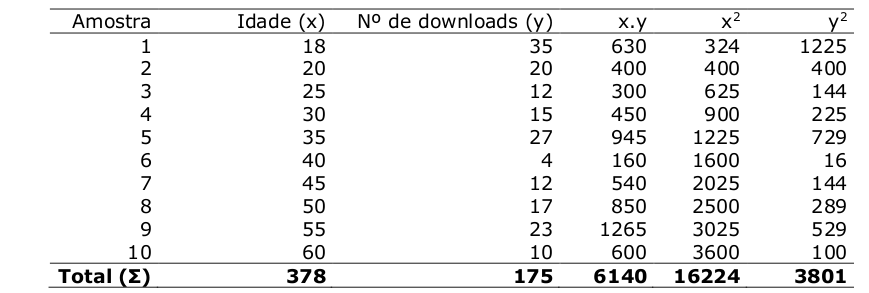
\includegraphics[width=10 cm]{20-2016.png}\newline

Qual alternativa representa a equação da Reta de Regressão, y=ax+b, para os dados coletados, onde $\bar x $ e $\bar y$ são as médias dos valores de x e y, e $a = \frac{\sum xy -n \bar x \bar y }{\sum x^2 -n(\bar x)^2 }$ e $b = \bar y - a\bar x$ ?\newline

a) y = 26.7762x − 0.2454

b) y = −0.2454x + 26.7762

c) y = −2.454x + 26.7762

d) y = −24.54x + 26.7762

e) y = 24.54x + 267.762\newline




\item (2015, 13) Um grupo de 10 pessoas é composto por 4 homens e 6 mulheres. Nesse caso,\newline

a) o número de maneiras de selecionar uma comissão de cinco pessoas é igual a $\frac{6!4!}{5!}$

b) o número de maneiras de selecionar uma comissão de três pessoas, contendo um homem e duas mulheres, é igual a $4! + \frac{6!}{2!}$

c) o número de maneiras de selecionar uma comissão de quatro pessoas na qual não constem homens é igual a $10! - 4!$

d) o número de maneiras de organizar as dez pessoas em fila indiana é igual a $ \frac{10!}{4!6!}$

e)o número de maneiras de organizar as dez pessoas em fila indiana, de forma que os homens sejam os quatro primeiros da fila, é igual a $4! 6!$\newline


\textbf{RESOLUÇÃO}

$\rule[1cm]{100cm}{1px}$


e)o número de maneiras de organizar as dez pessoas em fila indiana, de forma que os homens sejam os quatro primeiros da fila, é igual a $4! 6!$\newline







\textbf{CONTEÚDO}

$\rule[1cm]{100cm}{1px}$

a única possibilidade seria permutando os 4 homens primeiro e depois as 6 mulheres


\newpage



\item (2015, 18) Uma urna contém 10 bolas brancas e $n > 0$ bolas pretas. Duas bolas são retiradas sem reposição e ao acaso dessa urna. Dado que uma bola preta foi retirada na segunda extração, para que a probabilidade condicional de retirar uma bola branca na primeira extração seja igual a $\frac{1}{3}$, o valor de n deverá ser igual a:

a) 21

b) 25

c) 31

d) 32

e) 34\newline






\item (2015, 20) O tempo requerido para executar determinada tarefa foi medido em dois sistemas, A e B. Os tempos para o sistema A foram 8,19; 4,57; 3,38; 2,50; 3,60; 1,74. Já para o sistema B foram 5,36; 3,52; 0,62; 1,41; 0,64; 3,26. 

O teste t para amostras independentes apresentou o p-valor bilateral igual a 0,2343.

Ao nível de significância $\alpha=5 \%$ , consideram-se os dois sistemas estatisticamente distintos?\newline

a) Sim, pois o p-valor é maior que o nível de significância, o que significa que existe diferença significativa entre as médias de
tempo de execução entre os dois sistemas.

b) Sim, pois o p-valor é maior que o nível de significância, o que significa que não existe diferença significativa entre as médias
de tempo de execução entre os dois sistemas.

c) Não, pois o p-valor é maior que o nível de significância, o que significa que não existe diferença significativa entre as médias
de tempo de execução entre os dois sistemas.

d) Não, pois o p-valor é maior que o nível de significância, o que significa que existe diferença significativa entre as médias de
tempo de execução entre os dois sistemas.

e) Não, pois o p-valor é maior que a metade do nível de significância, uma vez que o teste é bilateral, não existindo diferença sig-
nificativa entre as médias de tempo de execução entre os dois sistemas.\newline








\item(2014, 9)Em uma pesquisa realizada com 1000 internautas sobre o acesso a dois sites de compras, A e B, observou-se que 350 internautas fazem compras em A, 500 fazem compras em B e 100 fazem compras
nos sites A e B.

Com base nessas informações, assinale a alternativa que apresenta, corretamente, o percentual dos intenautas entrevistados que não fazem compras nos sites A e B.\newline

a) 15\%

b) 25\%

c) 35\%

d) 45\%

e) 55\%\newline








\item(2014, 13)Suponha que o sistema de identificação de funcionários em uma empresa seja composto por um código com quatro dígitos numéricos.

Assinale a alternativa que apresenta, corretamente, a quantidade máxima de funcionários que essa empresa pode registrar com esse sistema de identificação, considerando dígitos numéricos distintos.

a) 3024

b) 5040

c) 6561

d) 9000

e) 10000\newline 

\textbf{RESOLUÇÃO}

$\rule[1cm]{100cm}{1px}$

A(10,4)= $\frac{(10!)}{(10-4)!}$

A(10,4)= $\frac{(10!)}{(6)!}$

A(10,4)= $10.9.8.7=5040$\newline

b) 5040\newline

\textbf{CONTEÚDO}

$\rule[1cm]{100cm}{1px}$


Arranjo (n,p) = $A(10,4)= \frac{(n!)}{(n-p)!}$
quando o número de objetos e maior que número de posições e a ordem importa utiliza-se aranjo




\newpage






\item(2014, 17)Considerando que a prova do POSCOMP da área de Matemática tem 20 questões de múltipla escolha, assinale a alternativa que apresenta, corretamente, o número de gabaritos possíveis das 20 questões, com 5 alternativas por questão, contendo uma única alternativa correta.

a) $\frac{5}{20}$

b)$\frac{20}{5}$

c) 5 x 20

d) $20^5$

e) $5^{20}$\newline 

\textbf{RESOLUÇÃO}

$\rule[1cm]{100cm}{1px}$

$5_1.5_2.5_3...5_{20}$

$5^{20}$\newline

e) $5^{20}$\newline 



\textbf{CONTEÚDO}

$\rule[1cm]{100cm}{1px}$

temos que para a primeira questão serão 5 alternativas para a segunda questão mais 5 alternativas assim com as duas primeiras teriíamos $5.5=25$ que e igual a $5^2$ expandiando a idéia para 20 questões temos $5^{20}$


\newpage
\item(2014, 18)Em um torneio de futebol local, há 8 times de iguais habilidades, e o desenvolvimento da competição é simples. Os times são divididos em grupos de 2, por meio de sorteio, e jogam entre si. Os times perdedores são eliminados e os vencedores avançam na competição. Os vencedores são novamente dividos
em grupos de 2, por sorteio, e jogam entre si. Esse procedimento vai até que reste um único time que é o
campeão.

Nessas condições, assinale a alternativa que apresenta, corretamente, a probabilidade de dois determinados times de futebol se enfrentarem durante o torneio.


a) $\frac{1}{10}$

b) $\frac{1}{8}$

c) $\frac{1}{6}$

d) $\frac{1}{4}$

e) $\frac{1}{2}$\newline






\item(2014, 19)Admita por hipótese que se encontram disponíveis 5 executivos e 4 executivas para a formação de comissões gerenciais em uma empresa multinacional.

Com base nessa hipótese, considere as afirmativas a seguir.

I. Podem-se formar 72 comissões gerenciais de 5 pessoas com pelo menos 2 executivas.

II. Podem-se formar 90 comissões gerenciais de 5 pessoas com exatamente 2 executivas.

III. Podem-se formar 60 comissões gerenciais de 5 pessoas com exatamente 3 executivos.

IV. Podem-se formar 81 comissões gerenciais de 5 pessoas com pelo menos 3 executivos.

Assinale a alternativa correta.

a) Somente as afirmativas I e II são corretas.

b) Somente as afirmativas I e IV são corretas.

c) Somente as afirmativas III e IV são corretas.

d) Somente as afirmativas I, II e III são corretas.

e) Somente as afirmativas II, III e IV são corretas.\newline




\item(2014, 20)Suponha que em uma empresa uma de suas máquinas de manufatura esteja sob avaliação de performance. Na produção de oito lotes de peças, a máquina apresentou a seguinte sequência de peças defeituosas por lote: 9, 3, 8, 8, 9, 8, 9, 18.

Nessas condições, assinale a alternativa que apresenta, corretamente, o desvio padrão de peças defeituosas em relação à média.

$( S= \sqrt{\frac{\sum( x - \bar x)^2}{N}}$ onde S é o desvio padrão, N é o número de elementos da amostra, x é o elemento da amostra e $\bar x$ é a média aritmética. )

a) 0

b) $\sqrt{120}$

c) $\sqrt{15}$

d) 9

e) 72







\item(2013, 17)Em uma urna com 12 bolas, todas têm o mesmo tamanho e o mesmo peso, 7 são vermelhas e 5 são azuis. Assinale a alternativa que apresenta, corretamente, quantas maneiras distintas existem de se extrair as 12 bolas, uma a uma, dessa urna.

a) 12

b) 792

c) 1908

d) 19008

e) 95040\newline 

\textbf{RESOLUÇÃO}

$\rule[1cm]{100cm}{1px}$

$C(12,7)=\frac{12!}{7!.(12-7)!}$

$C(12,7)=\frac{12!}{7!.5!}$

$C(12,7)=\frac{12.11.10.9.8.7!}{7!.5!}$

$C(12,7)=\frac{12.11.10.9.8}{5!}=792$\newline


b) 792\newline



\textbf{CONTEÚDO}

$\rule[1cm]{100cm}{1px}$

$C(n,p)=\frac{n!}{p!.(n-p)!}$ utilizada quanto a o numero e objetos e diferente do númeroo de posições e quando a ordem não importa




\newpage




\item(2013, 18) Suponha um único lance de um dado não viciado. Assinale a alternativa que apresenta, corretamente, a probabilidade de insucesso em obter um 2 ou um 5.

a)$\frac{1}{36}$

b)$\frac{1}{12}$

c)$\frac{1}{6}$

d)$\frac{1}{3}$

e)$\frac{2}{3}$ \newline





\textbf{RESOLUÇÃO}

$\rule[1cm]{100cm}{1px}$

$1-\frac{1}{6}-\frac{1}{6}$

$1-\frac{2}{6}$

$\frac{6-2}{6}$

$\frac{4}{6}=\frac{2}{3}$\newline

e)$\frac{2}{3}$ \newline
 

\textbf{CONTEÚDO}

$\rule[1cm]{100cm}{1px}$


Excluindo-se 2 e 5 dentro do total de possibilidades que é 6, temos 1,3 4, 5 que são 4 possibilidades das 6. Ficamos então com 4/6 e ao simplificar por 2 obtemos 2/3. Portanto, alternativa e 2/3.


\newpage


\item(2013, 20) Considere o conjunto de números definido a seguir.

\{2, 2, 3, 3, 3, 5, 5, 8, 8, 8, 8, 17\}

Assinale a alternativa que apresenta, corretamente, a relação entre a média aritmética simples (Ma), a
moda (MO) e a mediana (Me) desse conjunto.

a) ME = MO = MA

b) ME = MA $<$ MO

c) MO $>$ ME = MA

d) MO $>$ MA $>$ ME

e) MA $<$ ME $<$ MO\newline 

\textbf{RESOLUÇÃO}

$\rule[1cm]{100cm}{1px}$


média aritmética(Ma)2+2+3+3+3+5+5+8+8+8+8+17=72/12=6

moda(MO)=8

mediana(Me)=5

 MO $>$ MA $>$ ME\newline

d) MO $>$ MA $>$ ME\newline



\textbf{CONTEÚDO}

$\rule[1cm]{100cm}{1px}$

média:a soma dos termos dividido pela quantidade de termoas $\frac{n_1+n_2+n_3+n_{...}}{n}$

mediana: e que ocupa o centro da lista, se houver mais de um valor e feito uma mádia.

moda: e o valor que mais se repete.

\newpage






\item(2012, 12)Para aumentar a segurança no acesso às contas correntes de uma certa rede bancária, solicitou-se aos clientes que, além da senha numérica, fosse cadastrada outra senha composta por uma sequência de três sílabas distintas. Cada sílaba é composta por duas letras, sendo a primeira uma consoante e a segunda uma vogal.

Nessas condições, e considerando o alfabeto com 26 letras, assinale a alternativa que apresenta, correta-
mente, a quantidade de possíveis senhas a serem formadas.

a) 1.092.624

b) 1.103.130

c) 1.120.000

d) 1.124.760

e) 1.200.760\newline 

\textbf{RESOLUÇÃO}

$\rule[1cm]{100cm}{1px}$


5.21=105

105.104.103=1124760\newline

d) 1.124.760\newline

\textbf{CONTEÚDO}

$\rule[1cm]{100cm}{1px}$

temos 5 vogais e 21 consoantes, então para a priméira sílaba temos 5.21=105 para compor a segunda síliba temos 105-1 pois mão pode se repetir o promeiro dígito e 105-2 pelo mesmo motivo 




\newpage




\item(2012, 14)Considerando os coeficientes de correlação, relacione a coluna da esquerda com os respectivos diagramas de dispersão, na coluna da direita.

\includegraphics[width=10 cm]{2015.png}\newline


Assinale a alternativa que contém a associação correta.

a) I-A, II-B, III-E, IV-D, V-C.

b) I-A, II-E, III-C, IV-B, V-D.

c) I-B, II-A, III-D, IV-E, V-C.

d) I-B, II-A, III-E, IV-D, V-C.

e) I-C, II-A, III-D, IV-B, V-E.\newline





\item(2012, 19) Leia a definição a seguir.

Sejam E um experimento e Ω o espaço associado ao experimento. Uma função X que associa cada
elemento $ω\omega \in \Omega$ a um número real X($\omega$) é denominada variável aleatória.

Com base nessa definição e nos conhecimentos sobre distribuição de probabilidades, atribua V (verda-
deiro) ou F (falso) às afirmativas a seguir.

( ) Uma variável aleatória pode ser discreta ou contínua: discreta quando seus valores pertencem a um
conjunto enumerável de números reais, e contínua quando seus valores pertencem a um conjunto
não enumerável de números reais.

( ) Uma função probabilidade só assume valores negativos, e a soma das probabilidades, para todos os
valores possíveis da variável aleatória, tem que ser igual a 1.

( ) A função distribuição de probabilidade de uma variável aleatória discreta X é definida como
$P (X \leq x) $= F (x), onde $-\infty < x < \infty.$

( ) A cada variável aleatória está associada uma única função: a função probabilidade, na qual o domínio
são as probabilidades da variável e a imagem é o valor da variável no domínio.

( ) Qualquer função de uma variável aleatória é também uma variável aleatória. Isto é, se X é uma
variável aleatória então Y = $\varphi$(X) também é uma variável aleatória.
Assinale a alternativa que contém, de cima para baixo, a sequência correta.

a) V, F, V, V, F.

b) V, F, V, F, V.

c) V, F, F, V, F.

d) F, V, V, F, V.

e) F, V, F, V, F.\newline










\item(2011, 19)Zezinho aposta 6 números, dentre os 60 disponíveis, no jogo da mega-sena. Após o sorteio, Zezinho

observa que o resultado é formado por 6 números primos. Se, no momento de sua aposta, Zezinho tivesse essa informação, então a probabilidade de acerto de Zezinho seria de:

a) $\frac{1}{{13 \choose 6}}$

a) $\frac{1}{{17 \choose 6}}$

a) $\frac{1}{{19 \choose 6}}$

a) $\frac{1}{{29 \choose 6}}$

a) $\frac{1}{{59 \choose 6}}$\newline



\item(2011, 20)O código Morse usa dois símbolos: ponto e traço horizontal. Se as palavras desse alfabeto tiverem de 1 a 4 letras, é correto afirmar que o código Morse permitirá escrever:

a) 8 palavras.

b) 16 palavras.

c) 30 palavras.

d) 32 palavras.

e) 256 palavras.\newline
 

\textbf{RESOLUÇÃO}

$\rule[1cm]{100cm}{1px}$

2.4.8.16=30 \newline


c) 30 palavras.\newline



\textbf{CONTEÚDO}

$\rule[1cm]{100cm}{1px}$

para a primeira palavra tem uma letra no qual pode ser composta por o ponto ou traço $2$ na segunda temos duas letras podendo ser ponto ou traços $2^2$ assim por diante 

assim temos $2^1+2^2+2^3+2^4=30$



\newpage


\item(2010, 9)O dominó é um jogo com 28 peças, com dois números em cada peça, com todas as combinações de 0 a 6. Duas peças de dominó são sorteadas. A probabilidade de que tenham um número em comum é:

a) 1/7

b) 7/18

c) 1/2

d) 0,4

e) 21/28\newline 

\textbf{RESOLUÇÃO}


$\frac{21}{28}.\frac{12}{27} + \frac{7}{28}.\frac{6}{27} = \frac{7}{18}$\newline


b) 7/18\newline


\textbf{CONTEÚDO}

$\rule[1cm]{100cm}{1px}$



I) 2 Números diferentes na primeira peça

São 21 peças, entre as 28, com números diferentes; logo a probabilidade associada a essa hipótese é P1= 21/28.

Suponha que a primeira peça tenha os sido retirado. Entre as 27 peças restantes, há 6 que têm o número a e outras 6 que têm o número mesmo número P1igual=6/27+6/27=12/27. 


II) 2 Números iguais na primeira peça

São 7 peças com números iguais, logo a probabilidade associada a essa hipótese é P2=7/28.

Suponha que a primeira peça tenha sido retirada. Entre as 27 peças restantes, há 6 que têm o número. Logo, a probabilidade de que a segunda peça tenha o número é simplesmente P2igual=6/27.


A probabilidade total de que a segunda peça tenha um número igual ao da primeira pode ser calculada da seguinte forma: 

P/total = P1*P1|igual + P2*P2|igual= 21/28*12/27 + 7/28*6/27 = 7/18 

Logo, 7/18


\newpage



\item(2010, 11)De quantos modos 4 homens e 4 mulheres podem se sentar em 4 bancos de 2 lugares, se em cada banco deve haver um homem e uma mulher?

a) 64

b) 8!

c) $\frac{8!}{2!}$

d) 8.7.6.5

e) $16.24^2$\newline


\textbf{RESOLUÇÃO}

$\rule[1cm]{100cm}{1px}$

$Ch(4,2)=\frac{4!}{(4-2)!}=12$

$Cm(4,2)=\frac{4!}{(4-2)!}=12$

$2(12+12)$

arranjo=2.2.2.2=$2^4$=16 

$16.2.(12+12)$

$16.(24)^2$\newline

e) $16.24^2$\newline


\textbf{CONTEÚDO}

$\rule[1cm]{100cm}{1px}$

no primeiro momento temos a combinação dos homens Ch que seria a posição que os mesmos estão sentados em seguida as posições das mulheres Cm de depois somamos(24) mais a posição que os mesmos estão sentados pode ser hm ou mh assim multiplicamos por 2.(24), mais o primeiro banco pode ser ocupado por qualquer casal assim fazemos um arranjo com as posições dos casais no banco 
\newpage



\item(2010, 13)João e Manuel retiram, para cada um, um bilhete de uma urna em que há 60 bilhetes numerados de 1 a 60. A probabilidade de que o número retirado por João seja maior do que o de Manuel é:

a) 31/60

b) 60/59

c) 60\%

d) 50\%

e) 29/60 \newline







\item(2010, 15)Para calcular a média e o desvio padrão das notas de seus 30 alunos, um professor de estatística utiliza a soma das notas e a soma de seus quadrados, obtendo 180 para a primeira, e 1544, para a segunda. A média e o desvio padrão valem, respectivamente,

a) 4 e 6 

b) 6 e 9 

c) 6 e 4

d) 4 e 8 

e) 9 e 5\newline 

\textbf{RESOLUÇÃO}

$\rule[1cm]{100cm}{1px}$


* Cálculo da média:

$M =\sum \frac{x}{N}$

$M= \frac{180}{30} = 6$

M = 6

* Cálculo do desvio padrão:

$D= \sqrt{\frac{(\sum x^2)}{N} -E^2}$

$D= \sqrt{\frac{1544}{30} - 36}$

D = 3,93 

D = 4\newline


c) 6 e 4\newline


\textbf{CONTEÚDO}

$\rule[1cm]{100cm}{1px}$

média:a soma dos termos dividido pela quantidade de termoas $\frac{n_1+n_2+n_3+n_{...}}{n}$

desvio pdrão: $D= \sqrt{\frac{\sum (x_i - \bar x)^2}{n}}$

$x_i$: valor individual 

$\bar x$: valor da média 

n: número determos 


\newpage




\item(2010, 18)Um dado honesto tem duas faces pintadas de azul e as outras quatro, de amarelo. O dado é lançado três
vezes, anotando-se a cor da face obtida. A probabilidade de a cor obtida no primeiro lançamento ser igual
à obtida no terceiro lançamento é:

a) 2/3

b) 1/3

c) 50\%

d) 9/20

e) 5/9\newline 

\textbf{RESOLUÇÃO}

$\rule[1cm]{100cm}{1px}$


$\frac{1}{3}.\frac{1}{3}=\frac{1}{9}$

$\frac{2}{3}.\frac{2}{3}=\frac{4}{9}$

$\frac{1}{9}+\frac{4}{9}=\frac{5}{9}$\newline


e) 5/9\newline 



\textbf{CONTEÚDO}

$\rule[1cm]{100cm}{1px}$


temoa a probalidade de $\frac{2}{6}=\frac{1}{3}$ do lançamento ser azul e $\frac{4}{6}=\frac{2}{3}$ de ser amarelo no primeiro lance e a mesma probabilidade no terceiro então temos $\frac{1}{3}.\frac{1}{3}=\frac{1}{9}$ para o azul e $\frac{2}{3}.\frac{2}{3}=\frac{4}{9}$ para o amarelo então somando os dois temos $\frac{1}{9}+\frac{4}{9}=\frac{5}{9}$

\newpage




\item(2009, 9) Considere duas variáveis aleatórias discretas A e B independentes. Sejam $\partial_A^2$ e $\partial_B^2$ as variâncias de A e B respectivamente.\newline

Se K e P são constantes, o que pode ser dito a respeito da variância de \newline

(K + a) -   (p + b)? \newline

a) $\partial_A^2$ - $\partial_B^2$

b) $\partial_A^2$ + $\partial_B^2$  

c) (K + p) x ($\partial_A^2$ + $\partial_B^2$)

d) (K - p) x ($\partial_A^2$ - $\partial_B^2$)

e) (K x $\partial_A^2$) + (p x $\partial_B^2$)   \newline



\item(2009, 10) Qual é o número possível de anagramas que se pode montar com as letras da palavra
POSCOMP, mesmo que a palavra formada não exista? \newline


a) 7!

b) 7!/ (2! x 2!)

c) 3! x (2! + 2!)

d) 2! x 2! x 1! x 1! x 1!

e) 7! x 2! x 2! \newline 

\textbf{RESOLUÇÃO}

$\rule[1cm]{100cm}{1px}$



7!(quantidade de letras) / 2! . 2! (quantidade de repetições)



b) 7!/ (2! x 2!)\newline



\textbf{CONTEÚDO}

$\rule[1cm]{100cm}{1px}$

A palavra POSCOMP possui 7 letras mas 2 dessas letras se repetem que são o O e o P se não houvesse letras repetidas teriamos $7!$ mais a troca de posição das letras repetidas formam a mesma palavra tendo em vista esse aspecto retiramos as palavras repetidas sendo assim temos $\frac{7!}{2! . 2!}$



\newpage



\item(2009, 11) Seja X uma variável aleatória discreta. Sejam $x_1,x_2,...,x_n$ os valores que X pode
assumir e $p_1, p_2,..p_n$ a probabilidade de ocorrência de cada um destes valores. Neste
caso o valor esperado de X é dado por:\newline

a) $\sum x_i$ + $\sum p_i$

b) $\sum (x_i$ x $\sum p_i)$

c) $(\sum x_i)$ x $(\sum p_i)$

d) $\sum (x_i$ x $p_i)$

e) $\prod (x_i + p_i)$ \newline 

\textbf{RESOLUÇÃO}

$\rule[1cm]{100cm}{1px}$





\newline

d) $\sum (x_i$ x $p_i)$\newline

\textbf{CONTEÚDO}

$\rule[1cm]{100cm}{1px}$

temos que para cada valor de $x$ pode assumir qualquer valor ade $p$ então temos $x.p$ após isso somamos eles então inserimos o somatório

\newpage



\item(2009, 12) Chama-se palíndromo um número que não se altera quando invertida a ordem de seus
algarismos. Exemplos: 515, 7887, 30503. Quantos são os palíndromos de exatamente 5
algarismos?


a) 20

b) 500

c) 900

d) 1000

e) Nenhuma das respostas anteriores.\newline

\textbf{RESOLUÇÃO}

$\rule[1cm]{100cm}{1px}$

posição 1 - 9

posição 2 - 10

posição 3 - 10

9.10.10=900\newline

c) 900\newline


\textbf{CONTEÚDO}

$\rule[1cm]{100cm}{1px}$

para um palíndromo de 5 algarismos temos que o os 3 priméiros podem variar e os 2 últimos que que se repetir e também o número não pode comaçãr por zero para a primeira das 3 possibiidades temos 9 para a segunda e a terceira temos 10 e 10


\newpage




\item(2009, 16) Uma urna contém 6 bolas brancas e 4 bolas vermelhas iguais em tudo menos na cor.
Retiramos uma bola, anotamos a cor, recolocamos a bola na urna e retiramos mais uma
bola. Qual a probabilidade do resultado ser uma bola vermelha seguida de uma branca?

a) 10\%

b) 12\%

c) 18\%  

d) 24\%  

e) 36\%  \newline

\textbf{RESOLUÇÃO}

$\rule[1cm]{100cm}{1px}$

$\frac{6}{10}= \frac{3}{5}$

$\frac{4}{10}=\frac{2}{5}$

$\frac{3}{5}.\frac{2}{5}=\frac{6}{25}$

$\frac{6.4}{25.4}=\frac{24}{100}=24\%$\newline

d) 24\%\newline


\textbf{CONTEÚDO}

$\rule[1cm]{100cm}{1px}$

a probabilidade da bola a ser retirada ser branca é $\frac{6}{10}= \frac{3}{5}$ e de ser azul é $\frac{4}{10}=\frac{2}{5}$ com isso basta multiplicar as probabilidades $\frac{3}{5}.\frac{2}{5}=\frac{6}{25}$ multiplicamos em cima e em baixo por 4 para obtermos em termos percentuais então temos $24\%$ de obtermos esse seqência 







\newpage




\item(2008, 58) De quantos modos é possível comprar 4 picolés em uma loja que os oferece em
7 sabores distintos?

a) 210

b) 2.401

c) 35

d) 70

e) 11\newline
\textbf{RESOLUÇÃO}

$\rule[1cm]{100cm}{1px}$


$C(n,p)\frac{(n+p-1)}{p} = \frac{(7+4-1)}{4} = \frac{10!}{4!} $

$C(n,p)\frac{10.9.8.7.6!}{6!.4!} = \frac{10.9.8.7}{4.3.2} = 210 $ \newline

a) 210\newline


\textbf{CONTEÚDO}

$\rule[1cm]{100cm}{1px}$


(I) para 4 sabores iguais = 7 modos 

(II) para 3 iguais e 1 diferente  7x6 = 42 modos 

(III) para 2 iguais e dois iguais mas diferentes entre si  (7x6)/2 = 21 modos 

(IV)  para 2 iguais e dois diferentes 7x C(6,2) = 105 

(V)  para 4 diferentes  C(7,4) = 35 modos 

Total = (I) +(II) + (III) + (IV) + (V) = 210 

OU 

Combinação com repetição: 

$C(n,p)\frac{(n+p-1)}{p}$



\newpage



\item(2008, 59)O curso de Matemática de uma universidade tem 500 alunos. As disciplinas de Álgebra, Cálculo e Geometria têm 100, 120 e 80 alunos matriculados, respectivamente. O número de alunos matriculados em Álgebra e Geometria, mas não em Cálculo é 20. O número de alunos matriculados em Cálculo, mas não em Álgebra nem em Geometria é 55.

Considere as seguintes afirmativas.

I. A probabilidade de um aluno da universidade estar matriculado em pelo menos uma
dessas três disciplinas é menor que 50\%.

II. A probabilidade de um aluno matriculado em Cálculo estar também matriculado em
Geometria é 25\%.

III. Nenhum aluno está matriculado simultaneamente nas três disciplinas.
Com base na situação descrita, assinale a alternativa CORRETA.

a) Apenas a afirmativa II é verdadeira.

b) Apenas a afirmativa III é verdadeira.

c) Apenas a afirmativa I é verdadeira.

d) Todas as afirmativas são verdadeiras.

e) Todas as afirmativas são falsas.\newline

\textbf{RESOLUÇÃO}

$\rule[1cm]{100cm}{1px}$






\newline



\textbf{CONTEÚDO}

$\rule[1cm]{100cm}{1px}$





\newpage





\item(2008, 70)Considere que 14 cópias de uma mesma tarefa devem ser executadas paralelamente por
agentes idênticos, organizados em dois sistemas multiagentes, SMA-A e SMA-B. O
sistema SMA-A é formado por 16 agentes e o sistema SMA-B é formado por 32 agentes.
Seja C(m,p) a combinação de m elementos p a p.

Assinale fórmula que representa a quantidade de maneiras diferentes de escolher os
agentes, no caso em que pelo menos uma tarefa deve ser executada por algum agente
do sistema SMA-B.

a) C (48,14) -C(16,14)

b) C (32,1) $x$ C(47,13)

c) C (48,1) $x$ C(16,13)

d) C (32,1) $x$ C(48,13)

e) C (32,1) $x$ C(48,1) -C(32,14)\newline

\textbf{RESOLUÇÃO}

$\rule[1cm]{100cm}{1px}$

16 + 32 = 48

C(48,14) - C(16,14)\newline


a) C (48,14) - C(16,14)\newline



\textbf{CONTEÚDO}

$\rule[1cm]{100cm}{1px}$

total de agentes 16 + 32 = 48

dos 48 agentes escolhemoa 14 cópias = C(48,14)

C(48,14) - C(16,14) para que pelo menos uma tarefa seja executada pelo agente do sistema SMA-B




\newpage


\item(2007, 2)Para o processamento de um programa com 20 módulos independentes, pretende-se utilizar dois grupos de processadores em paralelo, X e Y . Para organizar esses grupos, contamos com 48 processadores, sendo que dois deles estão sujeitos a falhas. O grupo X somente pode conter oito processadores e nenhum deles pode apresentar falhas.
Nenhuma restrição foi especificada para o grupo Y . 

Nessa situação representada pela combinação de m elementos p a p e pelo arranjo de m elementos p a p, conclui-se que a quantidade de maneiras distintas de apresentar a organização dos processadores é igual a

a) C(48, 8) × C(40, 12)

b) A(48, 8) × A(40, 12)

c) C(46, 8) × C(40, 12)

d) A(46, 8) × A(40, 12)

e) A(46, 8) × C(40, 12)\newline



\item(2007, 18) Um professor de programação passa um trabalho e avisa à turma que vai utilizar um verificador automático para detectar trabalhos copiados. Os alunos descobrem que o verificador não é capaz de identificar a cópia se as linhas do programa não aparecem na mesma ordem. Além disso, eles também descobrem que uma rotina do trabalho de um de seus colegas continua funcionando corretamente se as linhas são trocadas de ordem, mas nenhuma linha aparece à distância maior do que 1 de sua posição original.

Indique o número de alunos que podem entregar uma cópia do trabalho quando n = 7 (incluindo o próprio autor do trabalho).

a) 32

b) 21

c) 14

d) 128

e) 64\newline

\textbf{RESOLUÇÃO}

$\rule[1cm]{100cm}{1px}$


6+5+4+3+2+1=21\newline



b) 21 \newline



\textbf{CONTEÚDO}

$\rule[1cm]{100cm}{1px}$

para o primeiro trablho temos 6 possobilidades de troca visto que pode ser trocada qualquer linha já no segundo temos apenas 5 visto que a posição anterior não pode ser trocada pois ficaria igual a primeira, aplicando a mesma lógica para os demais trabalhos 6+5+4+3+2+1=21

\newpage




\item(2007, 19) Suponha que o tempo de execução de um programa seja dado por uma variável aleatória T que assume os valores $10, 20, . . . , 100$ com distribuição de probabilidade uniforme $(i.e., P (T = 10k) = 1/10,$ para $k = 1, . . . , 10).$

A probabilidade de que o tempo total de duas execuções sucessivas e independentes desse programa não exceda 100 é

a) 0,50

b) 0,45

c) 0,40

d) 0,55

e) 0,60\newline


\item(2007, 20) Suponha agora que o programa é executado e se aguarda até 50 minutos para seu término. Se após esse perı́odo a execução não está terminada, então o programa é interrompido e reiniciado. A segunda execução sempre vai até o final. O tempo médio até o final da execução do programa quando utilizamos esse procedi mento é

a) 55

b) 62,5

c) 60

d) 49,5

e) 67,5\newline




\item(2006, 3) Quantos anagramas distintos podem ser formados com a palavra cochilo? Um
anagrama é uma palavra formada pela transposição das letras de outra palavra.
Iracema e Rmciaae são dois exemplos de anagramas distintos da palavra América.
Observe que a palavra formada não precisa ter sentido.

a) 5040

b) 2520

c) 630

d) 1260

e) 120\newline

\textbf{RESOLUÇÃO}

$\rule[1cm]{100cm}{1px}$


$\frac{7!}{2!.2!} = \farc{5040}{4}=1260$\newline

d) 1260\newline



\textbf{CONTEÚDO}

$\rule[1cm]{100cm}{1px}$


a palavra cochilo tem 7 letras com a letra a e a letra o se repetem 2 vezes, então se as letras repetidas mudarem de lugar formarão a mesma palavra, sabendo disso retiremos essas palavras. Temos 7! para todas as combinações, dividimos por 2! que são quantas vezes letras se repete em relação a c e por 2! denovo em relação ao o assim temos $\frac{7!}{2!.2!} = \frac{5040}{4}=1260$

\newpage




\item(2006, 11) O número de sequências de bits de comprimento 7 que contém um número par
de zeros é:

a) 128

b) 64

c) 32

d) 16

e) 8 \newline

\textbf{RESOLUÇÃO}

$\rule[1cm]{100cm}{1px}$

$C(7,2)=\frac{7!}{(7-2)!.2!}=21$

$C(7,4)=\frac{7!}{(7-4)!.4!}=35$

$C(7,6)=\frac{7!}{(7-6)!.6!}=7$

21+35+7=63

\newline



\textbf{CONTEÚDO}

$\rule[1cm]{100cm}{1px}$





\newpage






\item(2006, 16) Seis amigos reúnem-se para disputar partidas de xadrez em três tabuleiros diferentes. Calcule o número de partidas diferentes possı́veis levando-se em conta os tbuleiros mas não a cor das peças. Isto é, se os jogadores A e B jogam no primeiro tabuleiro é uma partida diferente deles jogando no segundo tabuleiro, mas quem joga com as brancas ou pretas é irrelevante.

a) 15

b) 30

c) 90

d) 120

e) 720 \newline

\textbf{RESOLUÇÃO}

$\rule[1cm]{100cm}{1px}$


ANULADA\newline



\textbf{CONTEÚDO}

$\rule[1cm]{100cm}{1px}$


ANULADA



\newpage






As duas questões a seguir são baseadas no seguinte enunciado:

Um algoritmo probabilı́stico A resolve problemas de dois tipos:

{Problemas do tipo 1}: os quais são resolvidos corretamente com probabilidade 3/4, e correspondem a 1/3 do total de problemas.

{Problemas do tipo 2}: os quais são resolvidos corretamente com probabilidade 1/2, e correspondem a 2/3 do total de problemas.


\item(2006, 17) i. Um problema é selecionado aleatoriamente e resolvido pelo algoritmo. Qual a probabilidade de que a resposta obtida seja correta?

a) 3/4

b) 5/12

c) 5/8

d) 7/12

e) 3/8 \newline

\textbf{RESOLUÇÃO}

$\rule[1cm]{100cm}{1px}$


$\frac{1}{3}.\frac{3}{4}+\frac{1}{2}.\frac{2}{3}$ 

$\frac{3}{12}.\frac{2}{6}=\frac{7}{12}$\newline

d) 7/12\newline


\textbf{CONTEÚDO}

$\rule[1cm]{100cm}{1px}$

primeiramente temos a probavilidade do primeiro algoritmo ser escolhido que e $\frac{1}{3}$ ou $\frac{2}{3}$ e aṕos isso a probabilidade do algoritmo resoover corretamente assim temos $\frac{1}{3}.\frac{3}{4}+\frac{1}{2}.\frac{2}{3}$ que no caso é $\frac{7}{12}$\newpage





\item(2006, 18) ii. Verifica-se, utilizando algum método determinı́stico, que a resposta encontrada pelo algoritmo está realmente correta. Qual a probabilidade de que o problema resolvido seja do tipo 1?

a) 4/9

b) 3/4

c) 7/12

d) 3/7

e) 7/3\newline





\item(2005, 5) Seja $T_{n, m}$ um tabuleiro xadrez $n \times m .$ Denominamos um circuito equestre em $T_{n, m}$ a um percurso de um cavalo, se movendo como num jogo de xadrez, que passa por cada uma das células de $T_{n, m}$ exatamente uma vez, e que começa e termina numa mesma célula (arbitrária). O número de circuitos equestre em $T_{5, 5}$ é. 


\includegraphics[width=10 cm]{2015.png}\newline


Figura 1: Exemplo de movimentos válidos de um cavalo.

a) 0

b) 1

c) 5

d) 25

e) 5! \newline




\item(2005, 15) Quantas cadeias de 7 bits contêm pelo menos 3 zeros consecutivos?

a) 81

b) 80

c) 48

d) 47

e) 16 \newline

\textbf{RESOLUÇÃO}

$\rule[1cm]{100cm}{1px}$


28+12+5+2+1=47 \newline

d) 47\newline


\textbf{CONTEÚDO}

$\rule[1cm]{100cm}{1px}$

contribuições exclusivas 

Com 7 = 1 cadeia de 7 

Com 6 = 4 - 2x1 =2 cadeias com 6 que não são de 7 

Com 5 = 12 - (3x1 +2x2)= 5 cadeias de 5 que não são de 6 ou 7 

Com 4 = 32 - (4x1 +3x2 + 2x5)= 12 cadeias de 4 

Com 3 = 80- (5x1 +4x2 + 3x5 + 2x12)= 28 cadeias de 3 que não são de 4, 5 ,6 ou7 

Logo a resposta é: 28+12+5+2+1=47 



\newpage




\item(2005, 19) Considere que todos os relés do circuito representado na figura abaixo funcionam independentemente e que a probabilidade de fechamento de cada rele é dada por $p .$ Qual a probabilidade de que haja corrente entre os terminais $A$ e $B ?$

\includegraphics[width=10 cm]{2015.png}\newline

a) $p^{2}$

b) 2$p^{2}$

c) $p^{4}$

d) $2 p^{2}-p^{4}$

e) 4$p$ \newline







\item(2004, 9) De quantas maneiras distintas podemos distribuir $m \geq k$ entavos entre $k$ meninas e $l$ meninos de maneira que cada menina receba pelo menos um centavo?


a) $\left(\begin{array}{c}{m} \\ {k}\end{array}\right)\left(\begin{array}{c}{m-k} \\ {\ell}\end{array}\right)$

b) $\left(\begin{array}{c}{m-k} \\ {k+\ell}\end{array}\right)$

c) $\left(\begin{array}{l}{m+\ell+k} \\ {k+\ell-1}\end{array}\right)$

d) $\left(\begin{array}{c}{m+\ell-1} \\ {k+\ell-1}\end{array}\right)$

e) $\left(\begin{array}{l}{m+\ell} \\ {k+\ell}\end{array}\right)$ \newline

     


\item(2004, 12) Num espaço finito de probabilidades $\Omega$ com distribuiçâo $\mathbb{P} : \Omega \rightarrow(0,1)$ , dados os eventos $A, B, C \subseteq \Omega$ quais das afirmações abaixo são verdadeiras?

(I) $\operatorname{Se} \mathbb{P}a)=1 / 2$ e $\mathbb{P}b)=3 / 5$ entâo $A$ e $B$ não são disjuntos.

(II) $\operatorname{Se} \mathbb{P}b)=1 / 3$ e $\mathbb{P}(A | b)=3 / 5$ entâo $A$ e $B$ são disjuntos. 

(III) $\operatorname{Se} \mathbb{P}a)=1 / 2, \mathbb{P}(B | a)=1$ e $\mathbb{P}(A | b)=1 / 2$ entâo $A \not\subseteq B$ e $\mathbb{P}b)=1$

IV) Se $A, B e C$ são eventos dois-a-dois independentes que ocorrem com probabilidade $1 / 2,1 / 4$ e $1 / 8,$ respectivamente, e $A$ ou $B$ ou $C$ ocorre com probabilidade $29/32$, então a probabilidade dos três eventos ocorrerem simultaneamente é $1/64$.


a) (I), (II)

b) (I), (III)

c) (I), (III), (IV)

d) (II), (III)

e) (III), (IV)\newline



\item(2004, 13) Quantas cadeias de 7 bits não contêm 3 zeros consecutivos?

a) 44

b) 48

c) 80

d) 81

e) 123\newline

\textbf{RESOLUÇÃO}

$\rule[1cm]{100cm}{1px}$






\newline



\textbf{CONTEÚDO}

$\rule[1cm]{100cm}{1px}$





\newpage


\item(2002, 5) Todos os convidados presentes num jantar tomam chá ou café. Treze convidados bebem café, dez bebem chá e 4 bebem chá e café. Quantas pessoas tem nesse jantar.

a) 19

b) 27

c) 23

d) 15

e) 10 \newline

\textbf{RESOLUÇÃO}

$\rule[1cm]{100cm}{1px}$

13-4=9

10-4=6

4+6+9=19\newline

a) 19\newline


\textbf{CONTEÚDO}

$\rule[1cm]{100cm}{1px}$

Temos que 13 pessoas bebem café e que 10 bebem chá e que 4 bebem café e cha 

assim pela teoria dos conjuntos temos que 13-4=9 bebem sómente café e que 10-4=6 bebem sómente chá 

assim temos 9+6+4=19 convidados

\newpage






\item(2002, 11) Uma prova de vestibular foi elaborada com 25 questões de múltipla escolha com 5 alternativas. O número de candidatos presentes à prova foi 63127. Considere a afirmação: 
Pelo menos 2 candidatos responderam de modo idêntico as k primeiras questões da prova. Qual é o maior valor de k para o qual podemos garantir que a afirmação é verdadeira.

a) 10

b) 9

c) 8

d) 7

e) 6 \newline

\textbf{RESOLUÇÃO}

$\rule[1cm]{100cm}{1px}$


$5^4 =   625 < 63127$\newline

$5^6 = 15625 < 63127$\newline

$5^7 = 78125 < 63127$\newline


e) 6 \newline


\textbf{CONTEÚDO}

$\rule[1cm]{100cm}{1px}$

O número de maneiras distintas de responder à primeira questão é 5, já que há 5 alternativas.

O número de maneiras distintas de responder às duas primeiras questões é 5 x 5 = 25.

O número de maneiras distintas de responder às k primeiras questões é $5^k$.

Para termos certeza de que pelo menos dois dos 63127 candidatos responderam de modo idêntico às k primeiras questões da prova, devemos ter 63127 > $5^k$.

Observando que $5^6$ = 15625 e $5^7$ = 78125, o maior valor de k que satisfaz a desigualdade acima é 6.


\newpage



\item(2002, 16) O número de strings binárias de comprimento 7 e contendo um par de zeros consecutivos é

a) 91

b) 92

c) 94

d) 95

e) 90 \newline
\textbf{RESOLUÇÃO}

$\rule[1cm]{100cm}{1px}$


1111111 1x  

0111111 7x  

0101111 5x  

0110111 4x  

0111011 3x  

0111101 2x  

0111110 1x  

0101011 3x  

0101101 2x  

0110101 2x  

0101110 1x  

0110110 1x  

0111010 1x  

0101010 1x


1 + 7 + 5 + 4 + 3 + 2 + 1 + 3 + 2 + 2 + 1 + 1 + 1 + 1 = 34 

$2 ^7 - 34 = 128 - 34 = 94$\newline


c) 94\newline


\textbf{CONTEÚDO}

$\rule[1cm]{100cm}{1px}$

Os 'Nx' são o número de possibilidades de não ocorrência da combinação da cdadeia 00.

assim temos $2^7$ que são todas as combinaçẽs - a possobolidade de não ocorrerem = todas as possibilidades que ocorrem 


\newpage




\item(2002, 17) A média aritmética de uma lista de 50 números é 50. Se dois desses números, 51 e 97, forem suprimidos dessa lista a média dos restantes será


a) 50

b) 49

c) 51

d) 47

e) 40 \newline

\textbf{RESOLUÇÃO}

$\rule[1cm]{100cm}{1px}$


$\frac{S_{50}}{50}=50$

$50.50=2500$

$\frac{2500-51-97}{48}=\frac{2352}{48}=49$\newline

b) 49\newline


\textbf{CONTEÚDO}

$\rule[1cm]{100cm}{1px}$


$S_{50}=$ soma dos 50 primeiros múmeros 

$M_{50}=$ média dos 50 primeiros números 

assim temos que a soma dos 50 primeiros números dividido por 50 é a mádia de 50, então temos que os 50 primeiros números multiplicado pela média será a soma dos números:

$M_{50}=\frac{S_{50}}{50}=50$ = $50.50$ = $2500$

assim temos que 2500 é a soma dos 50 primeiros números agora subtraimos os números suprimidos que são 51 e 97 assim temos e subtraímos 2 do total de números:

$M_{48}=\frac{2500-51-97}{48}=\frac{2352}{48}=49$


\newpage




\item(2002, 19)Numa prova de múltipla escolha com 10 questões e 4 alternativas qual a chance (probabilidade) de um aluno apenas “chutando as respostas” conseguir “gabaritar” a provar (acertar todas as questões).

a) 1$/ 10^{4}$

b) 1$/ 4^{20}$

c) 1$/ 2^{20}$

d) 1$/ 10^{8}$

e) 1$/ 4^{15}$ \newline

\textbf{RESOLUÇÃO}

$\rule[1cm]{100cm}{1px}$

$4.4.4.4...4=4^{10}$

$(2^2)^{10}$ = $2^{20}$

$\frac{1}{2^{20}}$\newline

c) 1$/ 2^{20}$\newline


\textbf{CONTEÚDO}

$\rule[1cm]{100cm}{1px}$

para cada questão temos 4 possibilidades então temos $4.4.4.4...4=4^{10}$. Podemos reescrever de outra forma $(2^2)^{10}$ = $2^{2.10}$ assim para que o aluno acerte todas as questões $\frac{1}{2^{20}}$

\newpage











\end{enumerate}

\newpage
\section{GRAFO}
\begin{enumerate}


\item (2018, 14) Seja um código de Hamming sistemático com a seguinte matriz de comprovação tal
que H =$(-P^T|I_r)$:\newline

H=$\Bigg(
    \begin{array}{ccccccc}
    1 & 1 & 0 & * & * & * & * \\
    0 & 1 & 1 & * & * & * & * \\
    1 & 0 & 1 & * & * & * & * \\
\end{array}\Bigg)$\newline

Transmite-se a palavra código Y=0000000 e, durante a transmissão, se produzem erros nas
posições 2, 3, 4 e 5. Que mensagem de usuário descodificaríamos?

a) X = 0100

b) X = 0111

c) X = 0011

d) X = 0010

e) X = 1001\newline



\item (2018, 17)Considere o grafo G abaixo e as afirmações feitas sobre G:

\includegraphics[width=10cm]{grafo2018.png}\newline

I. O grafo é planar.

II. O menor caminho direcionado medido em número de arcos entre os nós D e F tem comprimento
2.

III. DABCEF representa uma ordenação topológica válida dos nós do grafo.

IV. Existe algum caminho direcionado entre D e todos os outros nós do grafo.

V. O maior componente fortemente conexo de G é composto por um único nó, ou seja, não existe
em G um par de nós distintos x e y que tenha um caminho direcionado entre x e y e um
caminho direcionado entre y e x.\newline

Quais estão corretas?\newline

a) Apenas II e III.

b) Apenas I, II e IV.

c) Apenas I, III e V.

d) Apenas I, II, III e V.

e) I, II, III, IV e V.


item (2015, 7) Considere o seguinte problema de programação linear: maximize $2 x_1 +x_2$ , sujeito a $x_1 + x_2 =4$, $x_1 \geq 0, x_2 \geq 0.$

O problema dual associado pode ser formulado como:\newline

a) minimize $2 y_1 + 3 y_2 +4 y_3$ , sujeito a $y_1 + y_2 \geq 3$, $y_1 + y_3 \geq 1$, $y_1 \geq 0, y_2 \geq 0, y_3 \leq 0.$

b) minimize $4 y_1 + 3 y_2 +2 y_3$ , sujeito a $y_1 + y_2 \geq 2$, $y_1 + y_3 \geq 1$, $y_1 \geq 0, y_2 \geq 0, y_3 \leq 0.$

c) minimizey $1 + y_2 +4 y_3$ , sujeito a $y 1 + y_2 \geq 4$, $y_1 + y_3 \geq 1$, $y_1 \in R$ , $y_2 \geq 0, y_3 \leq 0.$

d) minimize $4 y_1 + 3 y_2 +2 y_3$ , sujeito a $y_1 + y_2 \geq 1$, $y_1 + y_3 \geq 2$, $y_1 \in R , y_2 \geq 0$, $y_3 \geq 0.$

e) minimize $4 y_1 + 3 y_2 +2 y_34$ , sujeito a $y_1 + y_2 \geq 2$, $y_1 + y_3 \geq 1$, $y_1 \in R , y_2 \geq 0, _3 \leq 0$.\newline





\item (2015, 19) Considere o grafo G=( N , a) dado a seguir.\newline

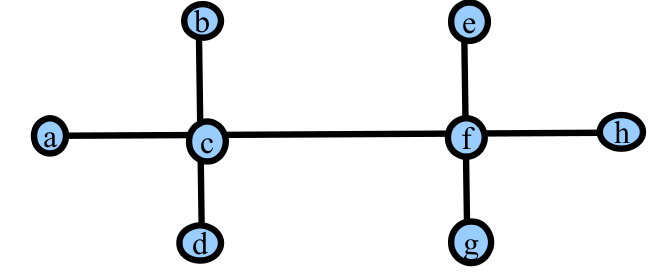
\includegraphics[width=10 cm]{19-2015.png}\newline

Pode-se, então, concluir que\newline

a) $2|A|$ = $\sum_{i \in N}$ $d_i +1$ onde $d_i$ denota o grau do i-ésimo nó.

b) G=( N , a) é euleriano.

c) G =( N , a) não é conexo.

d) H =$(Ñ, Ã )$ é um subgrafo de G=( N , a) , onde Ñ =$\{a , c , f , h \}$ e $A=\{\{a , c\}, \{c , f \}, \{ f , h\}\}$.

e) G=( N , a) não é planar.


\item(2011, 13) Considere o grafo a seguir.

\includegraphics[width=10 cm]{2015.png}\newline


O grafo representa a relação:

a) R = \{(1, 1), (1, 2), (1, 3), (3, 1), (4, 3)\}

b) R = \{(1, 1), (1, 2), (1, 3), (3, 1), (3, 4)\}

c) R = \{(1, 1), (1, 3), (2, 1), (3, 1), (3, 4)\}

d) R = \{(1, 1), (1, 2), (1, 3), (3, 4), (4, 3)\}

e) R = \{(1, 1), (1, 3), (2, 1), (3, 1), (4, 3)\}\newline






\item(2011, 18)Sejam 10 cidades conectadas por rodovias, conforme o grafo a seguir.


\includegraphics[width=10 cm]{2015.png}\newline

Um vendedor sai de uma das cidades com o intuito de visitar cada uma das outras cidades uma única vez
e retornar ao seu ponto de partida. Com base no grafo e nessa informação, considere as afirmativas a
seguir.

I. O vendedor cumprirá seu propósito com êxito se sair de uma cidade par.

II. O vendedor cumprirá seu propósito com êxito se sair de uma cidade ímpar.

III. O vendedor não cumprirá seu propósito com êxito se sair de uma cidade par.

IV. O vendedor não cumprirá seu propósito com êxito se sair de uma cidade ímpar.\\

Assinale a alternativa correta.\\

a) Somente as afirmativas I e II são corretas.

b) Somente as afirmativas I e IV são corretas.

c) Somente as afirmativas III e IV são corretas.

d) Somente as afirmativas I, II e III são corretas.

e) Somente as afirmativas II, III e IV são corretas.\newline




\item(2005, 17) O número máximo de nós no nı́vel i de uma árvore binária é:
(Considere o nı́vel da raiz igual a 1.)

a) $2^{i+1}, i \geq 0$

b) $2^{i-1}, i \geq 1$

c) $2^{i}, i \geq 1$

d) $2^{i}+1, i \geq 1$

e) $2^{i}-1, i \geq 1$ \newline

\newpage

\end{enumerate}





























\end{document}















$
\left \{ \begin{matrix} 
\end{matrix} \right.$ \newline



\includegraphics[width=10 cm]{2015.png}\newline




$
f(n) = \left [ \begin{matrix} 
    \begin{array}{cccc}
    3 & 0 & 0 & 0 \\
    a & 2 & d & e \\
    b & 0 & 1 & 0 \\
    c & 0 & f & 0 \\
\end{array}
\end{matrix} \right ]$ \newline



$\rule[1cm]{100cm}{1px}$\newpage
